\documentclass{beamer}	
\mode<presentation>
 
\usepackage{pdfpages}
\usepackage{fancyvrb}
\usepackage{chemarr}

\usepackage{amsmath}		%% mathematics typesetting
\usepackage{amssymb}
 
\usepackage{epigraph}   %% nice setting of quotations


\usepackage{ulem}

\usepackage{booktabs}

\usepackage{siunitx} %% tpyeset SI units

\usepackage{CJKutf8} %% typeset Chinese characters

\usepackage{pdfpages}%% include pdfs


\DeclareMathAlphabet{\mathcalligra}{T1}{calligra}{m}{n}


% Color and Theme. Can be changed. However, this one's quite nice.
\usetheme{Madrid}
\definecolor{theme}{rgb}{0.84,0,0.21}
\usecolortheme[named=theme]{structure}


%%  Title information
\title[M01.3 Flüssigkeiten und Gase]{M01.3 Aerodynamik, Hydrodynamik, \\ Viskosität und Grenzflächeneffekte}
\author[melanie.stefan@medicalschool-berlin.de]{M01 Physik für Mediziner*innen}
\institute[]{Prof. Melanie Stefan - melanie.stefan@medcialschool-berlin.de}
\date{WiSe 2022/23}
 

% Table of contents to pop up at the beginning of each section
\AtBeginSection[]
{
  \begin{frame}<beamer>
    \frametitle{Outline}
    \tableofcontents[currentsection,currentsubsection]
  \end{frame}
}
 
\beamertemplatenavigationsymbolsempty

\begin{document}


 { \usebackgroundtemplate{
\includegraphics[width=1.2\paperwidth]{MSB_Titelseite.pdf}} 
\begin{frame}

 \maketitle 

$\,$\\[6cm] 


\end{frame} 
}
 
 

%% Hook
\begin{frame}
\frametitle{Wie ist es auf dem Mauna Kea?}

\begin{columns}[c]

\begin{column}{5cm}

\begin{center}

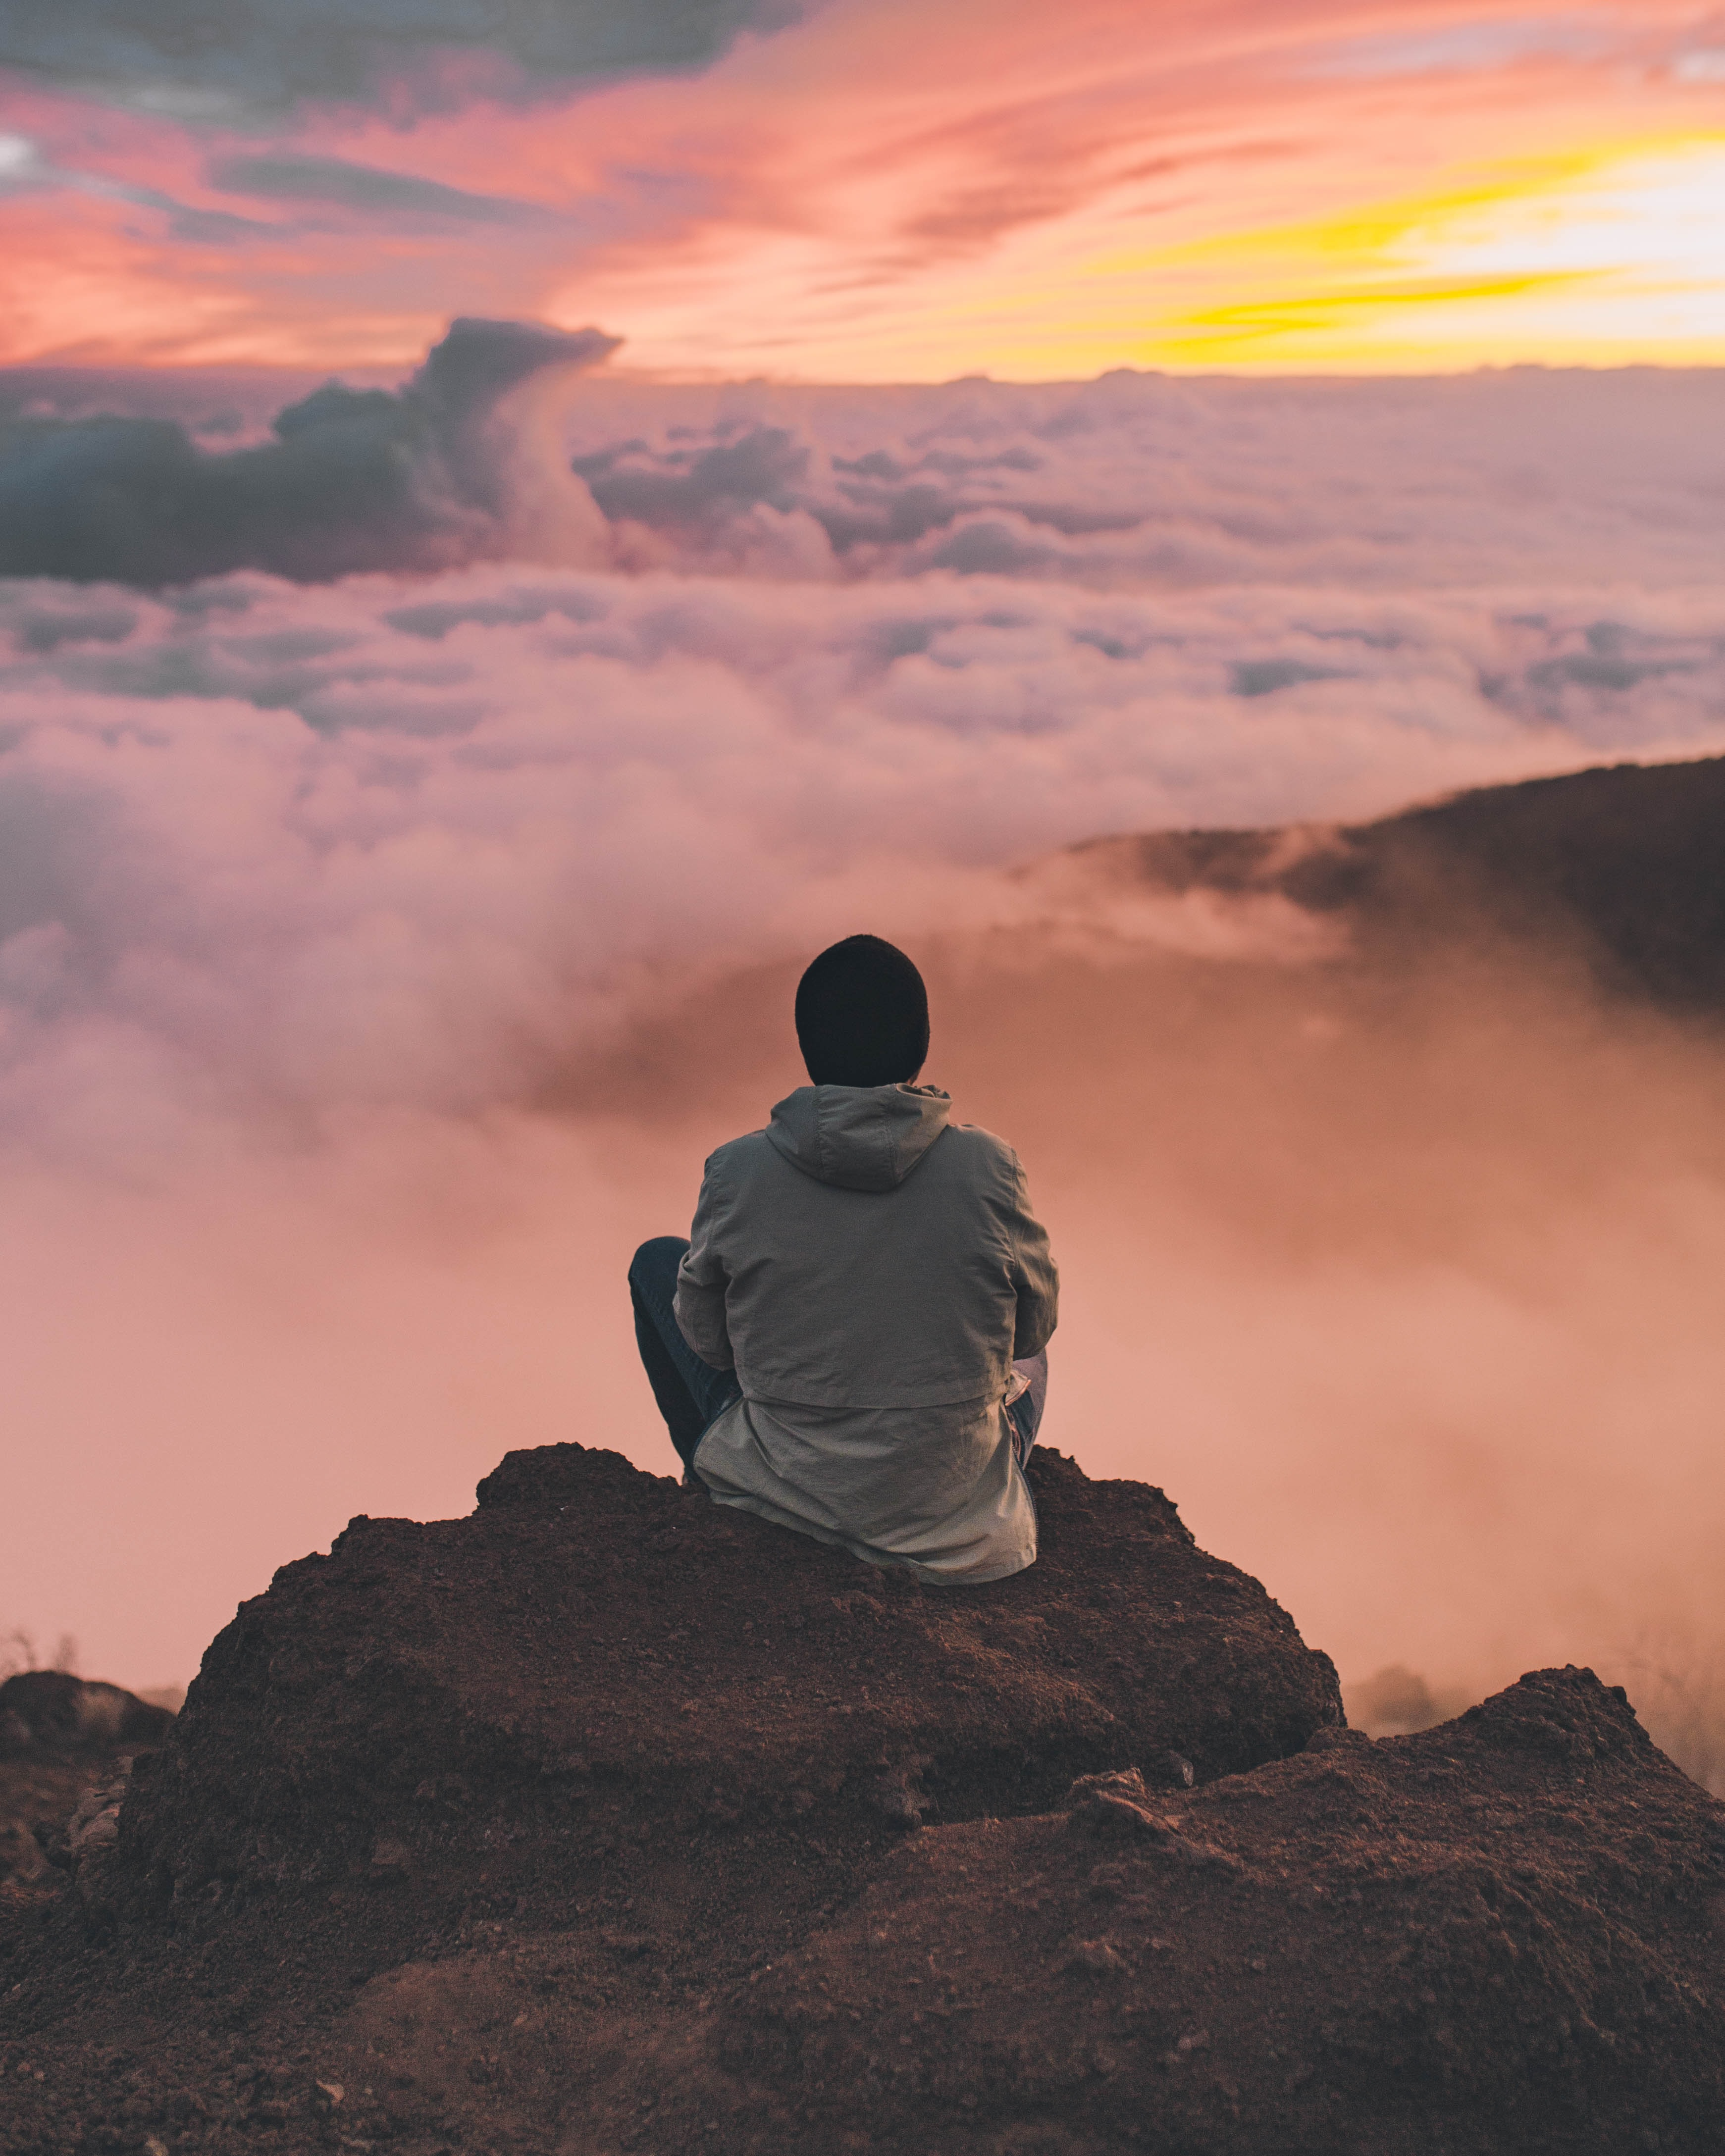
\includegraphics[width=\textwidth]{maunakea.jpg}

\end{center}

\end{column}

\begin{column}{5cm}


\epigraph{I traveled to the top of Mauna Kea one of the largest mountains in the world, although most of the mountain lies under water. The clouds surrounded my view point and it felt like I was entering into heaven.}{Ian Stauffer, Unsplash\\ \url{https://unsplash.com/photos/uftqFbfWGFY}}


\end{column}

\end{columns}

\end{frame}


\begin{frame}
\frametitle{Wie ist es auf dem Mauna Kea?}

\begin{columns}[c]

\begin{column}{5cm}

\begin{center}

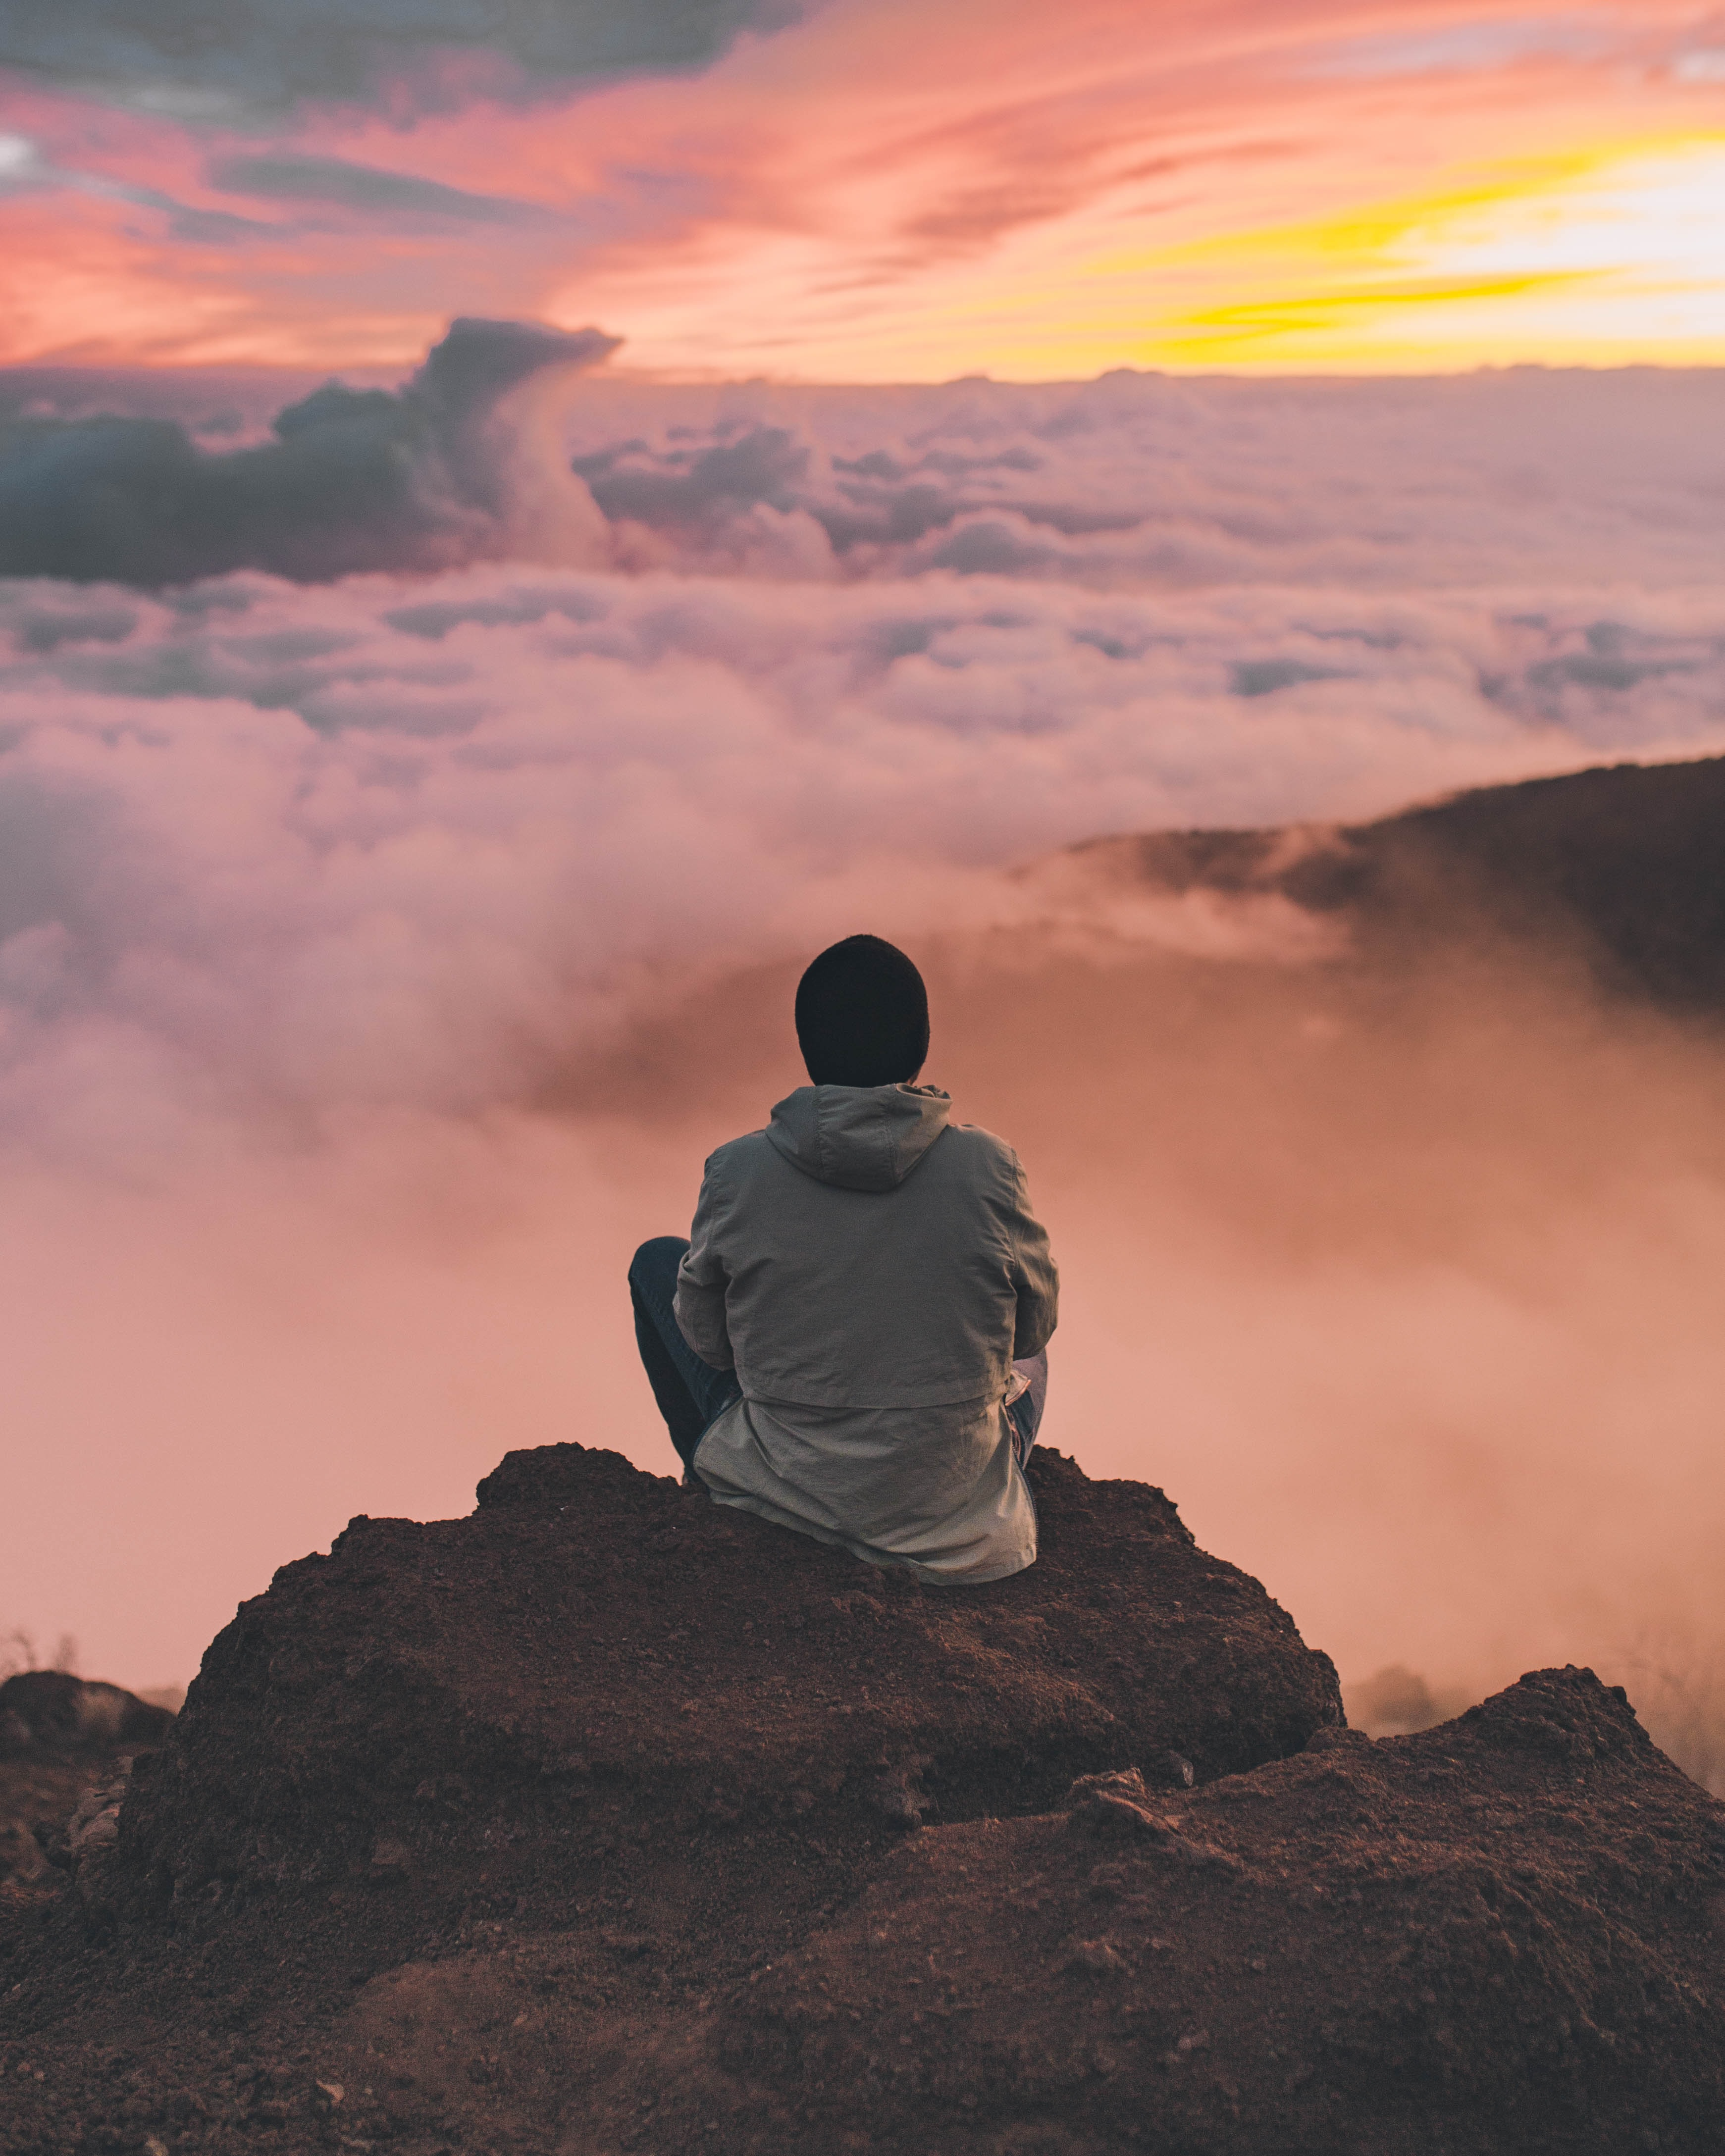
\includegraphics[width=\textwidth]{maunakea.jpg}

\end{center}

\end{column}

\begin{column}{5cm}

%% %% Keck observatory info
  \epigraph{Everyone who ascends to the summit of Mauna Kea feels [\dots] mild headaches, shortage of breath, nausea, fatigue, loss of memory, lack of concentration, lack of appetite and inablility to get to sleep.}{CFHT.\\ Working at High Altitude \\ \url{https://www.cfht.hawaii.edu/ObsInfo/HighAltitude/}}

\end{column}

\end{columns}

\end{frame}
 



%% TLIA

{
  \usebackgroundtemplate{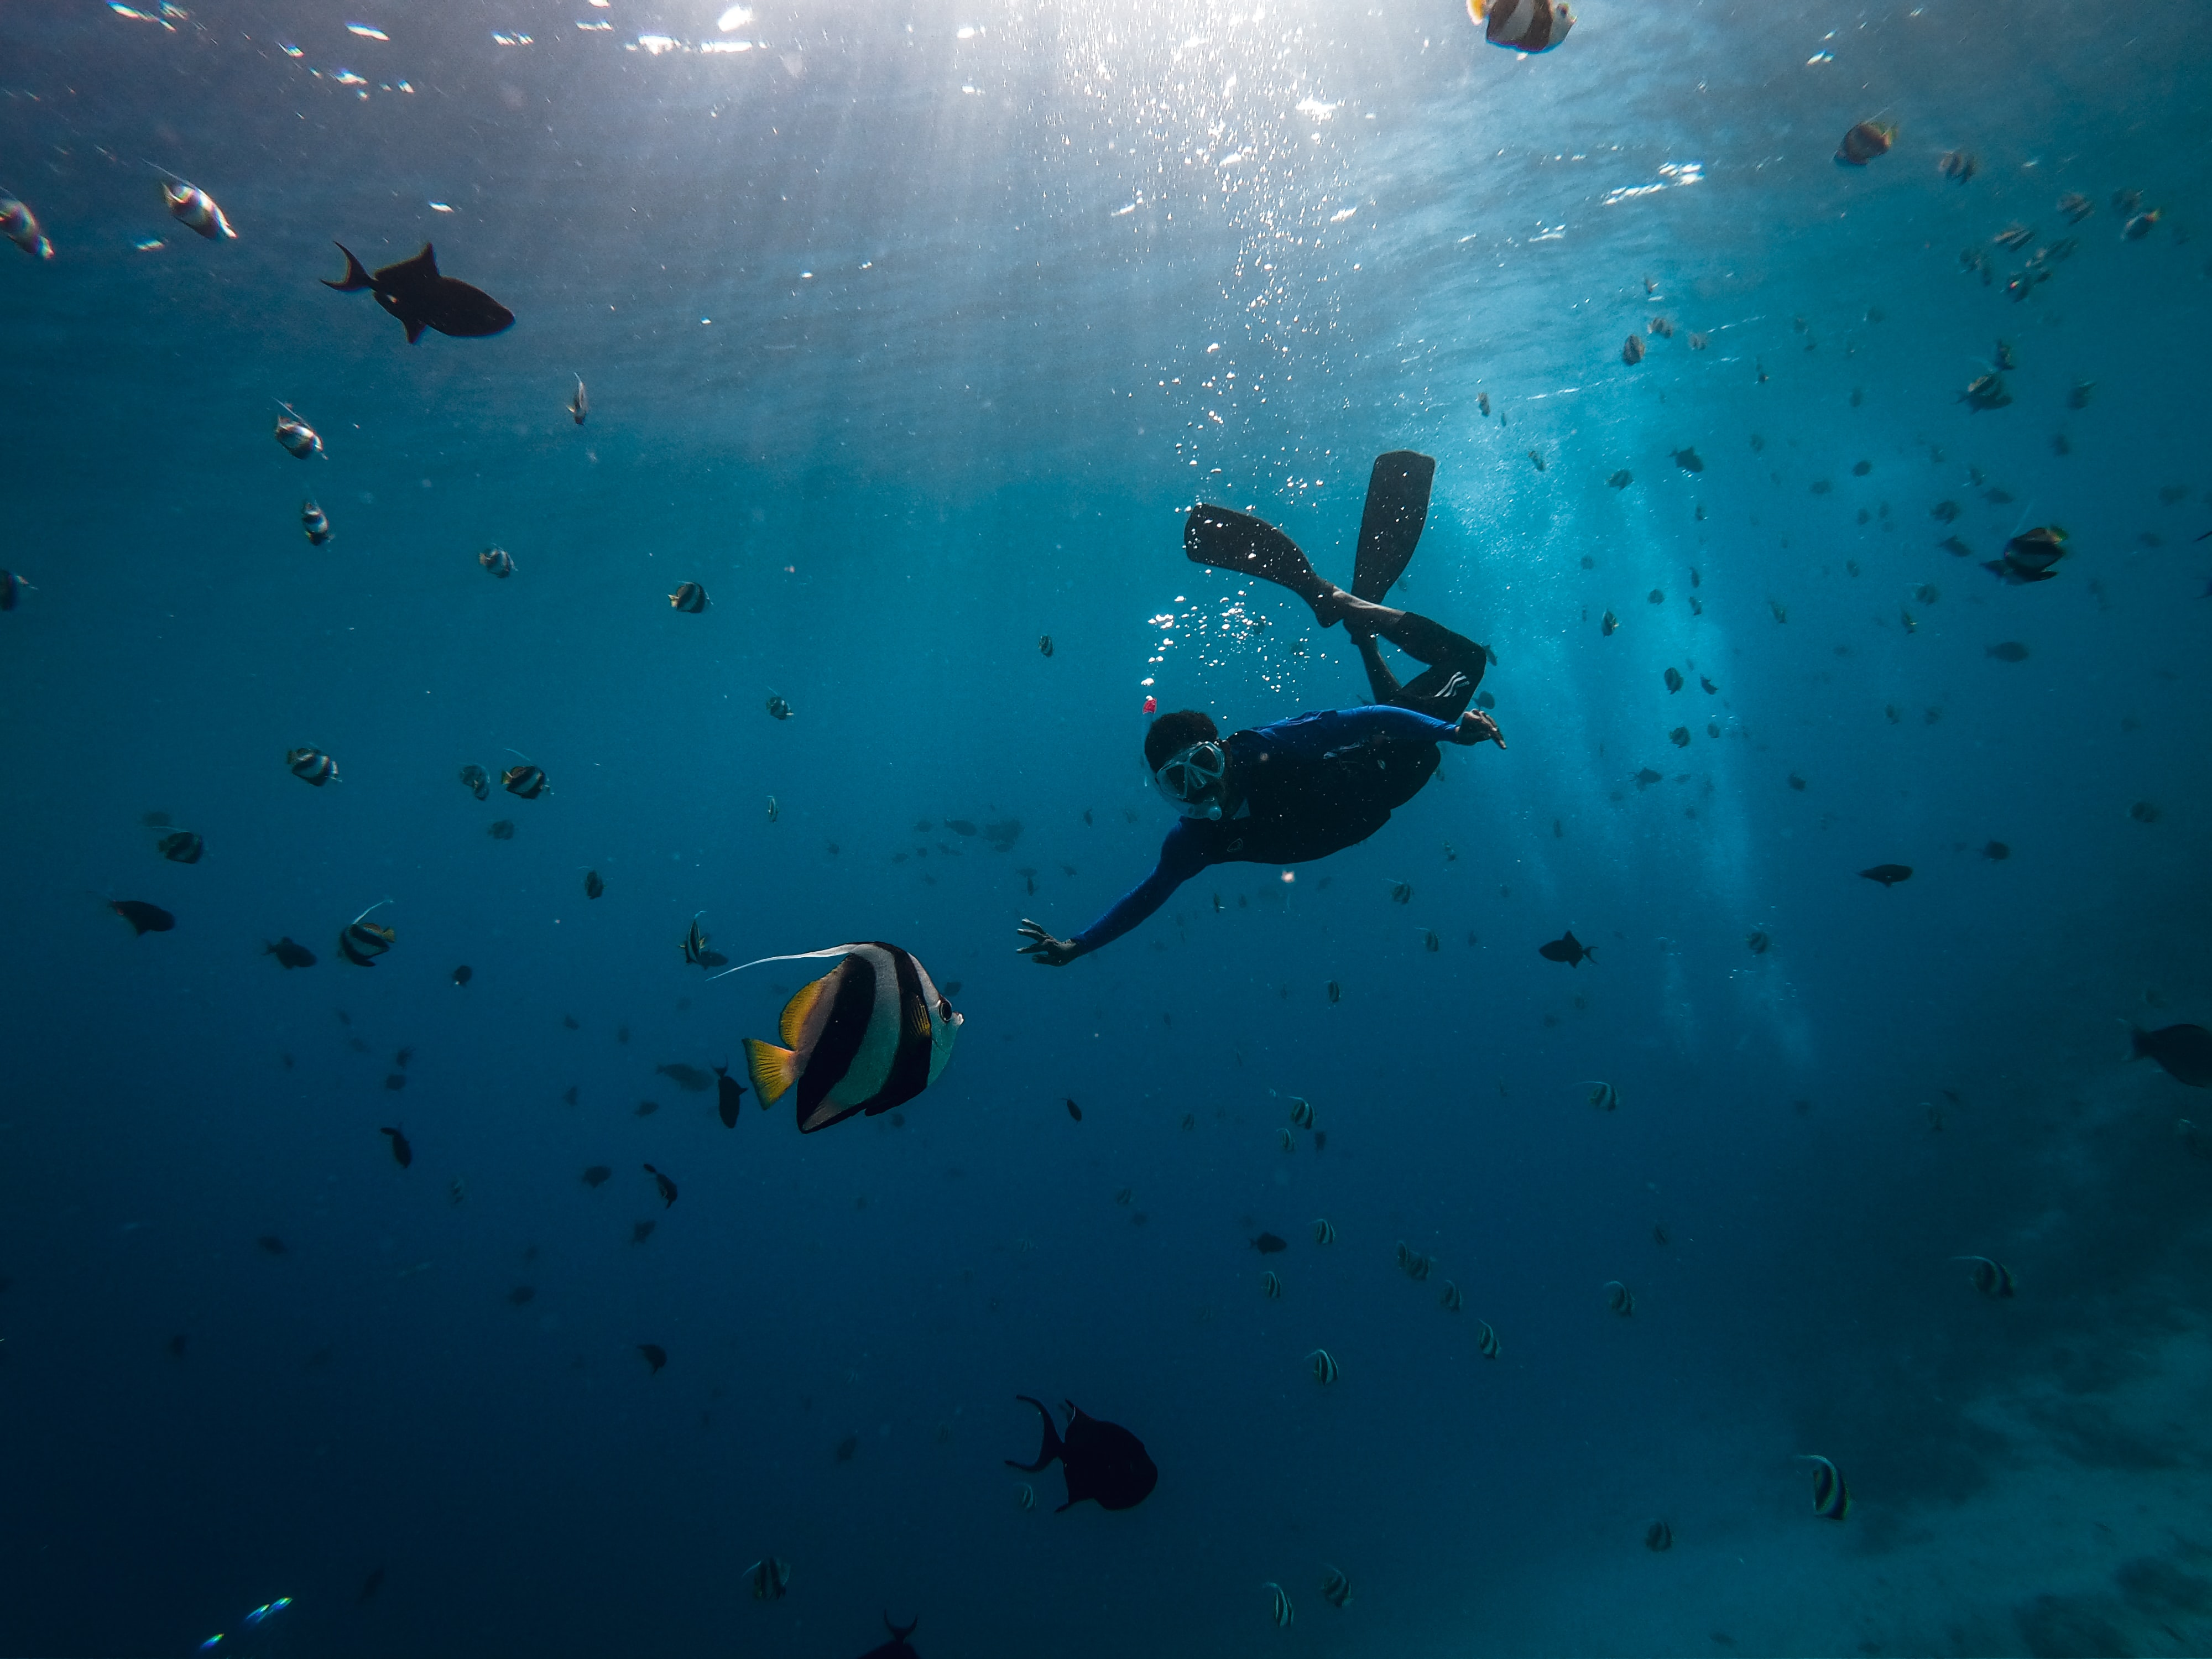
\includegraphics[width=1.4\paperwidth]{taucher.jpg}}

\begin{frame}[plain]

\frametitle{In dieser Vorlesung geht es um \dots}

\textcolor{white}{Bewegung von Flüssigkeiten und Gasen \\ und damit einhergehende Kräfte}

\vfill

 
\end{frame}
}


%% Learning Objectives
 
\begin{frame}

\frametitle{Nach dieser Vorlesung sollten Sie:}



\begin{block}{Wissen:}
\begin{itemize}
%%%%%
\item
Eigenschaften von Flüssigkeiten und Gasen erklären
\item
Druck definieren, Stempeldruck erklären
\item
Luftdruck erklären 
\item
Schweredruck in Flüssigkeiten und Auftrieb erklären
\item
Auswirkungen von Druck auf den menschlichen Organismus erklären
%%%%%
\item
Volumenstrom, Strömungswiderstand, Strömungsleitwert definieren 
\item
Kontinuitätsgleichung kennen 
%%%%%
\item
Kohäsion und Adhäsion definieren
\item
Den Kapillareffekt erklären und Beispiele geben
\item
Oberflächenspannung definieren
\end{itemize}

\end{block}

\end{frame}

\begin{frame}

\frametitle{Nach dieser Vorlesung sollten Sie:}
 



\begin{block}{Können:}
\begin{itemize}
\item
Druck und Auftrieb berechnen
\item
Luftdruck an verschiedenen Orten abschätzen
\item
Schweredruck im Wasser abschätzen
%%%%%%%
\item
Volumenstrom, Strömungswiderstand, Strömungsleitwert berechnen
\item
Die Kontinuitätsgleichung anwenden
\item
Strömungsfelder durch Stromlinien darstellen
\item
Prinzipien der Strömung im Blutkreislauf und in der Atmung erkennen
\item
Den Bernoulli-Effekt mit Alltagsgegenständen demonstrieren
\item
Die Kirchhoff-Gesetze anwenden
\item
Das Hagen-Poiseuille Gesetz anwenden
%%%%%%%
\item
Erklären, warum Händewaschen in einer viralen Pandemie wichtig ist
\end{itemize}
\end{block}

\end{frame}

\begin{frame}

\frametitle{Nach dieser Vorlesung sollten Sie:}
 

 


\begin{columns}[c]

\begin{column}{7cm}
\begin{block}{Fühlen:}

\begin{itemize}
\item
Die eigene Intuition im Hinblick auf Flüssigkeiten und Gase hinterfragen
\item
Die Augen offen halten für hydrodynamische und aerodynamische Effekte im Alltag und in der Medizin
\end{itemize}

\end{block}

\end{column}

\begin{column}{4cm}
\begin{center}
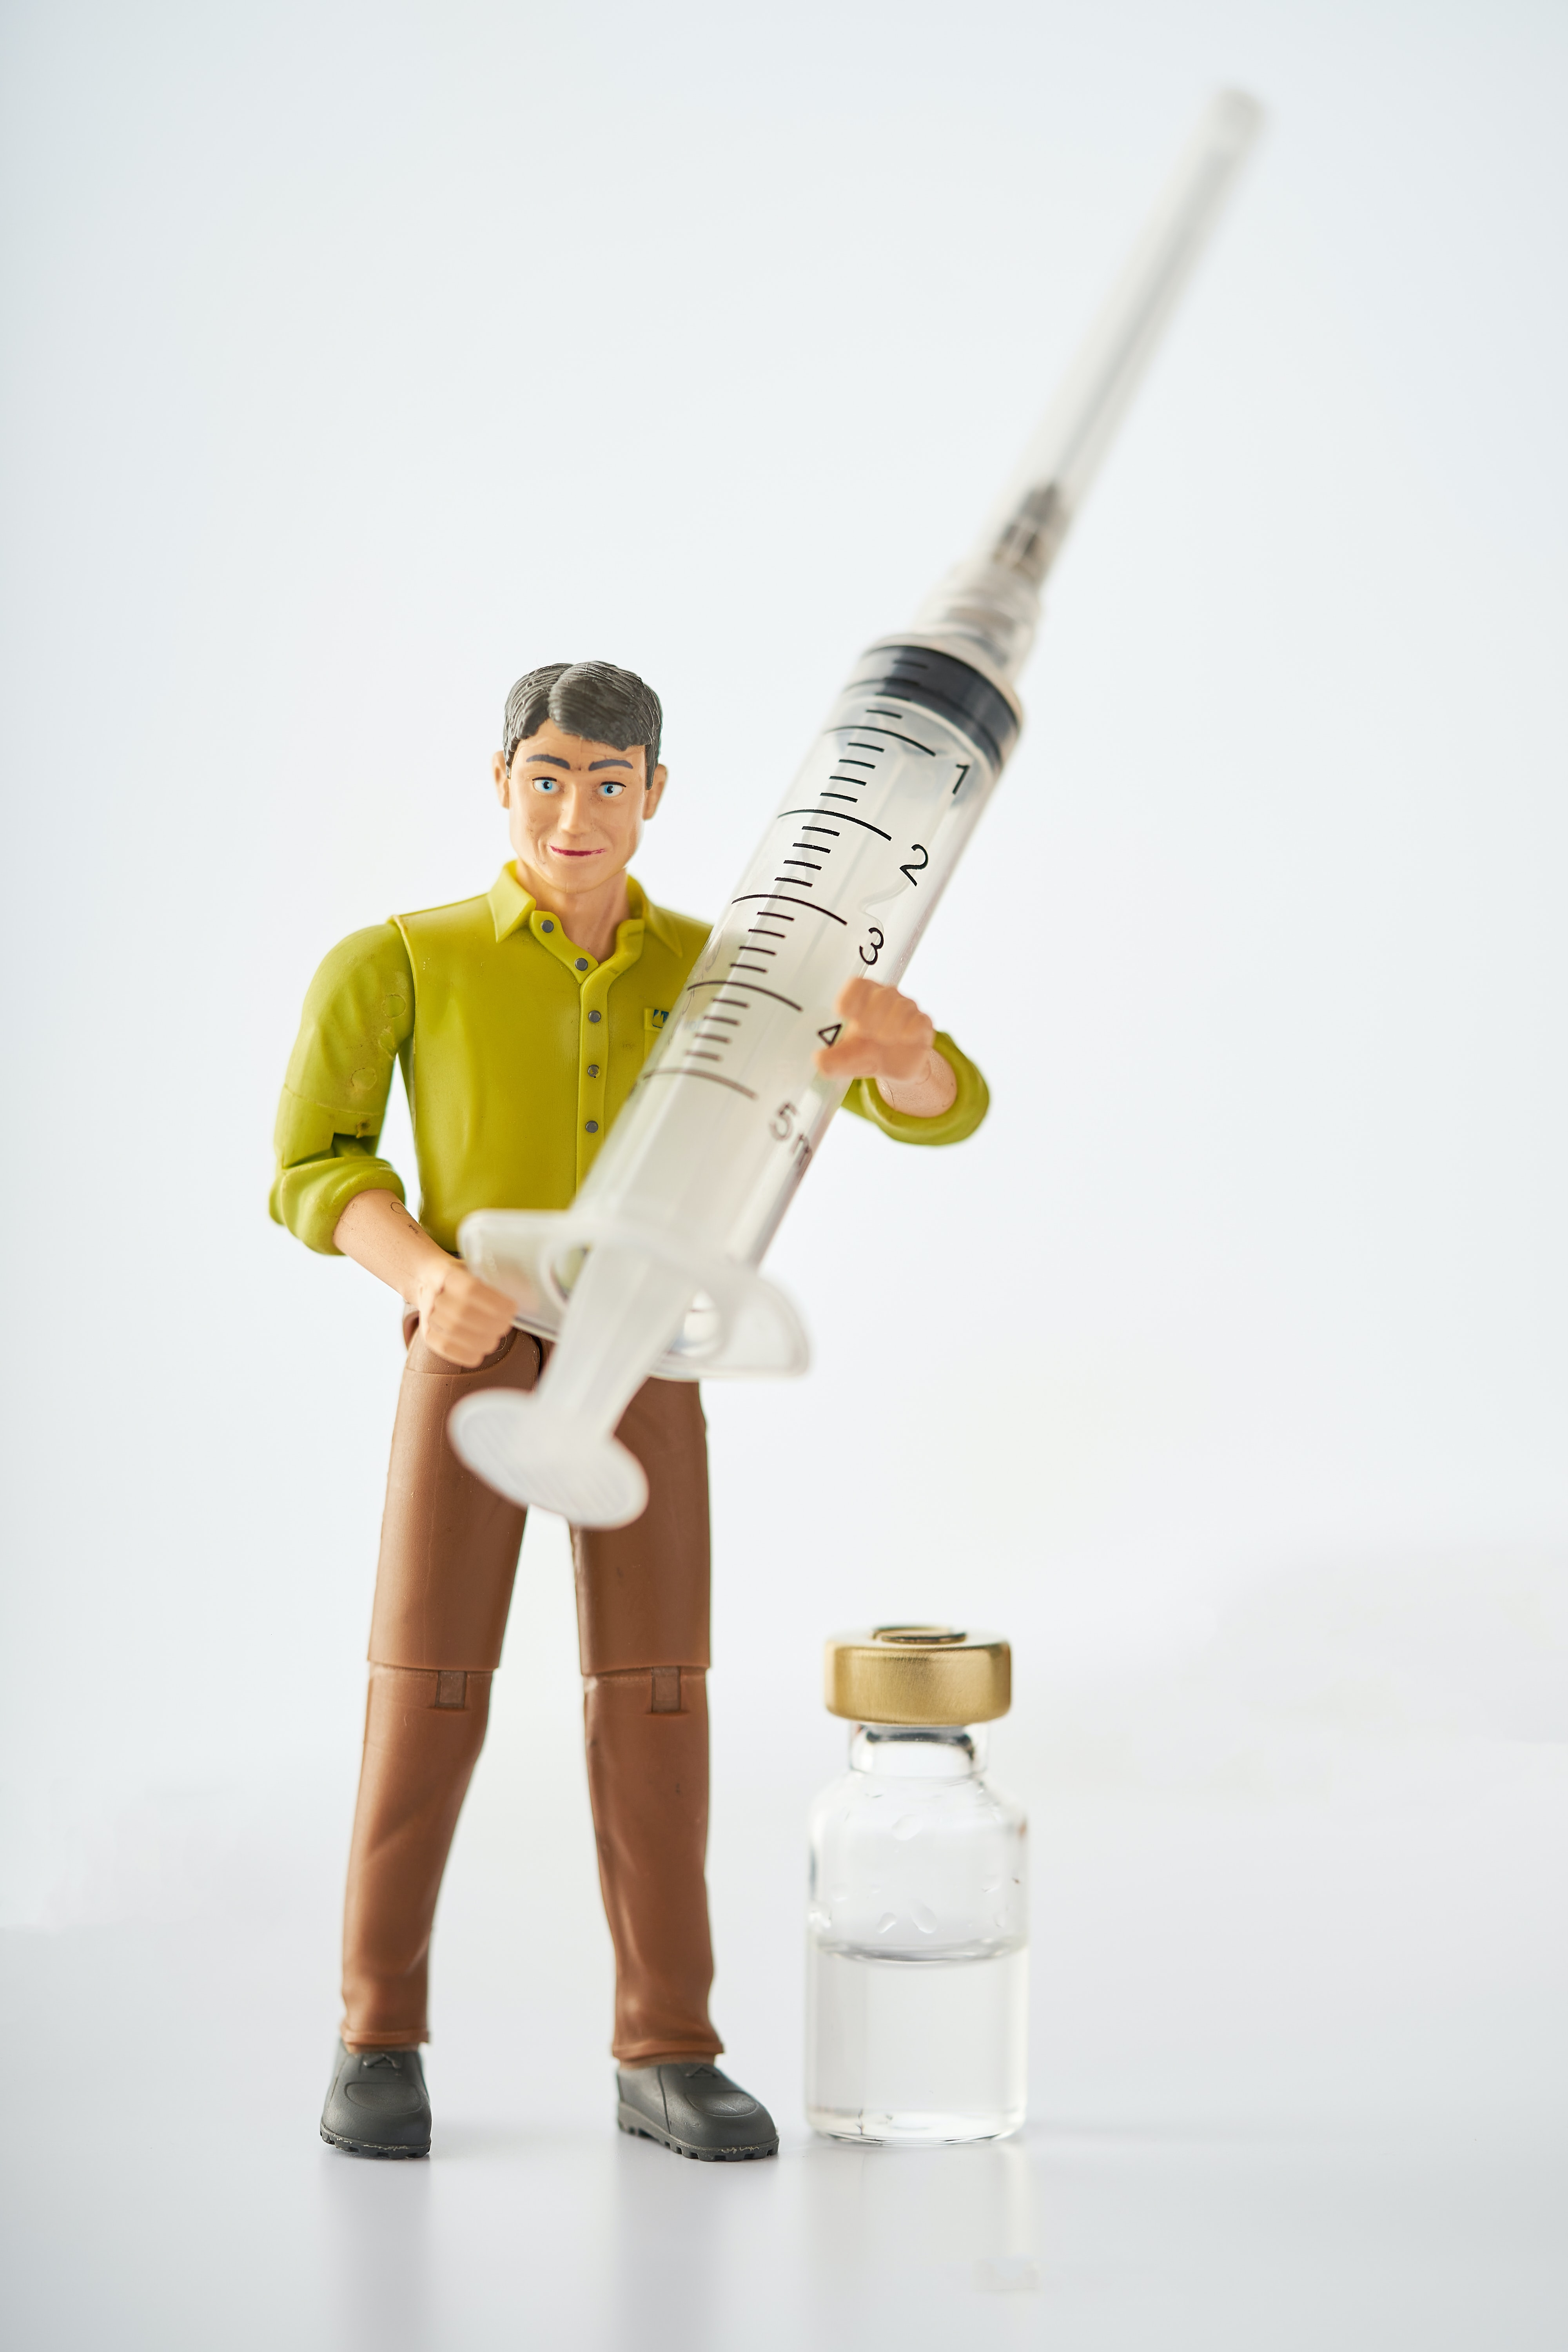
\includegraphics[width=\textwidth]{action_figure_needle.jpg}
\end{center}

\end{column}
\end{columns}



 \end{frame}

%% Main Body

\section{Druck}




%% Druck definieren

\begin{frame}
\makebox[\linewidth]{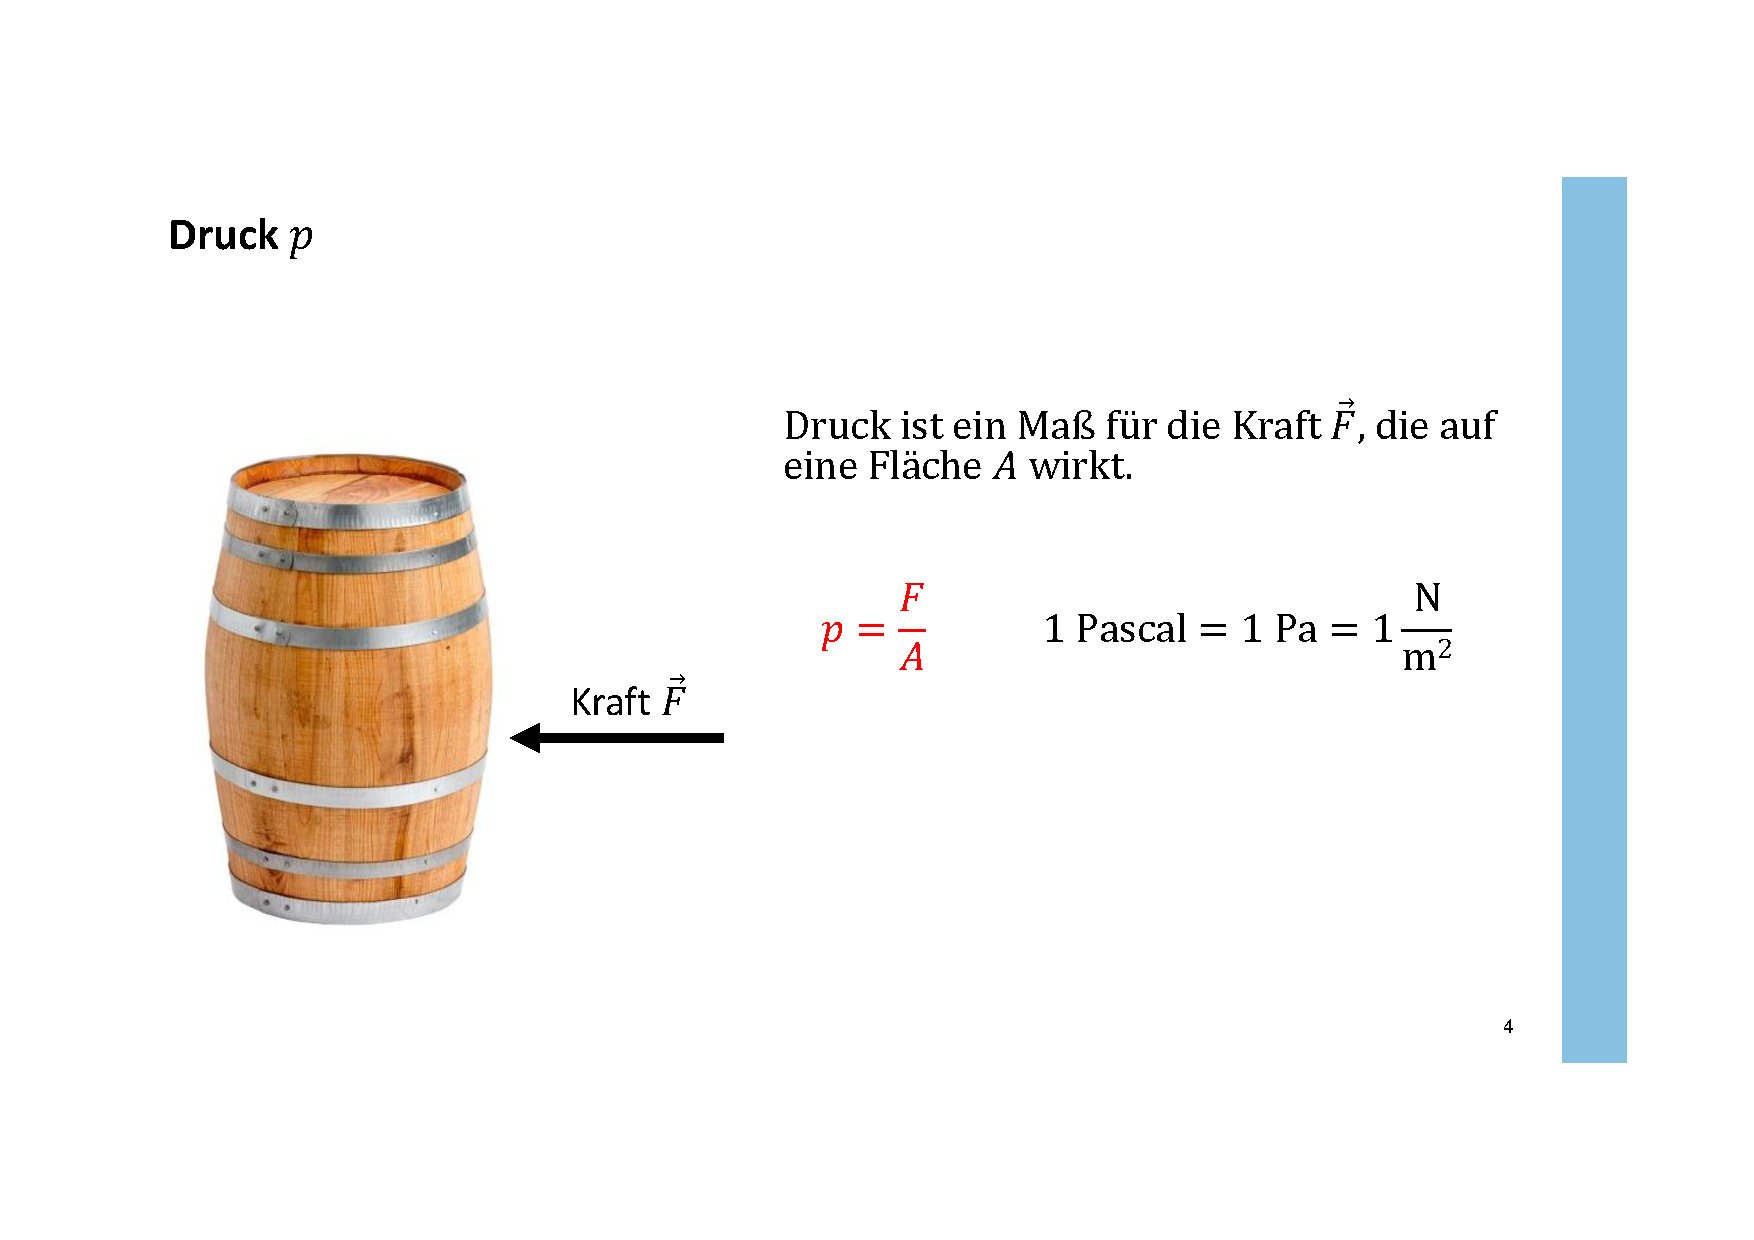
\includegraphics[width=\textwidth]{Walter_Druck_Definition.pdf}}
\end{frame}


\begin{frame}
\frametitle{Druck}

\begin{columns}[c]

\begin{column}{5cm}
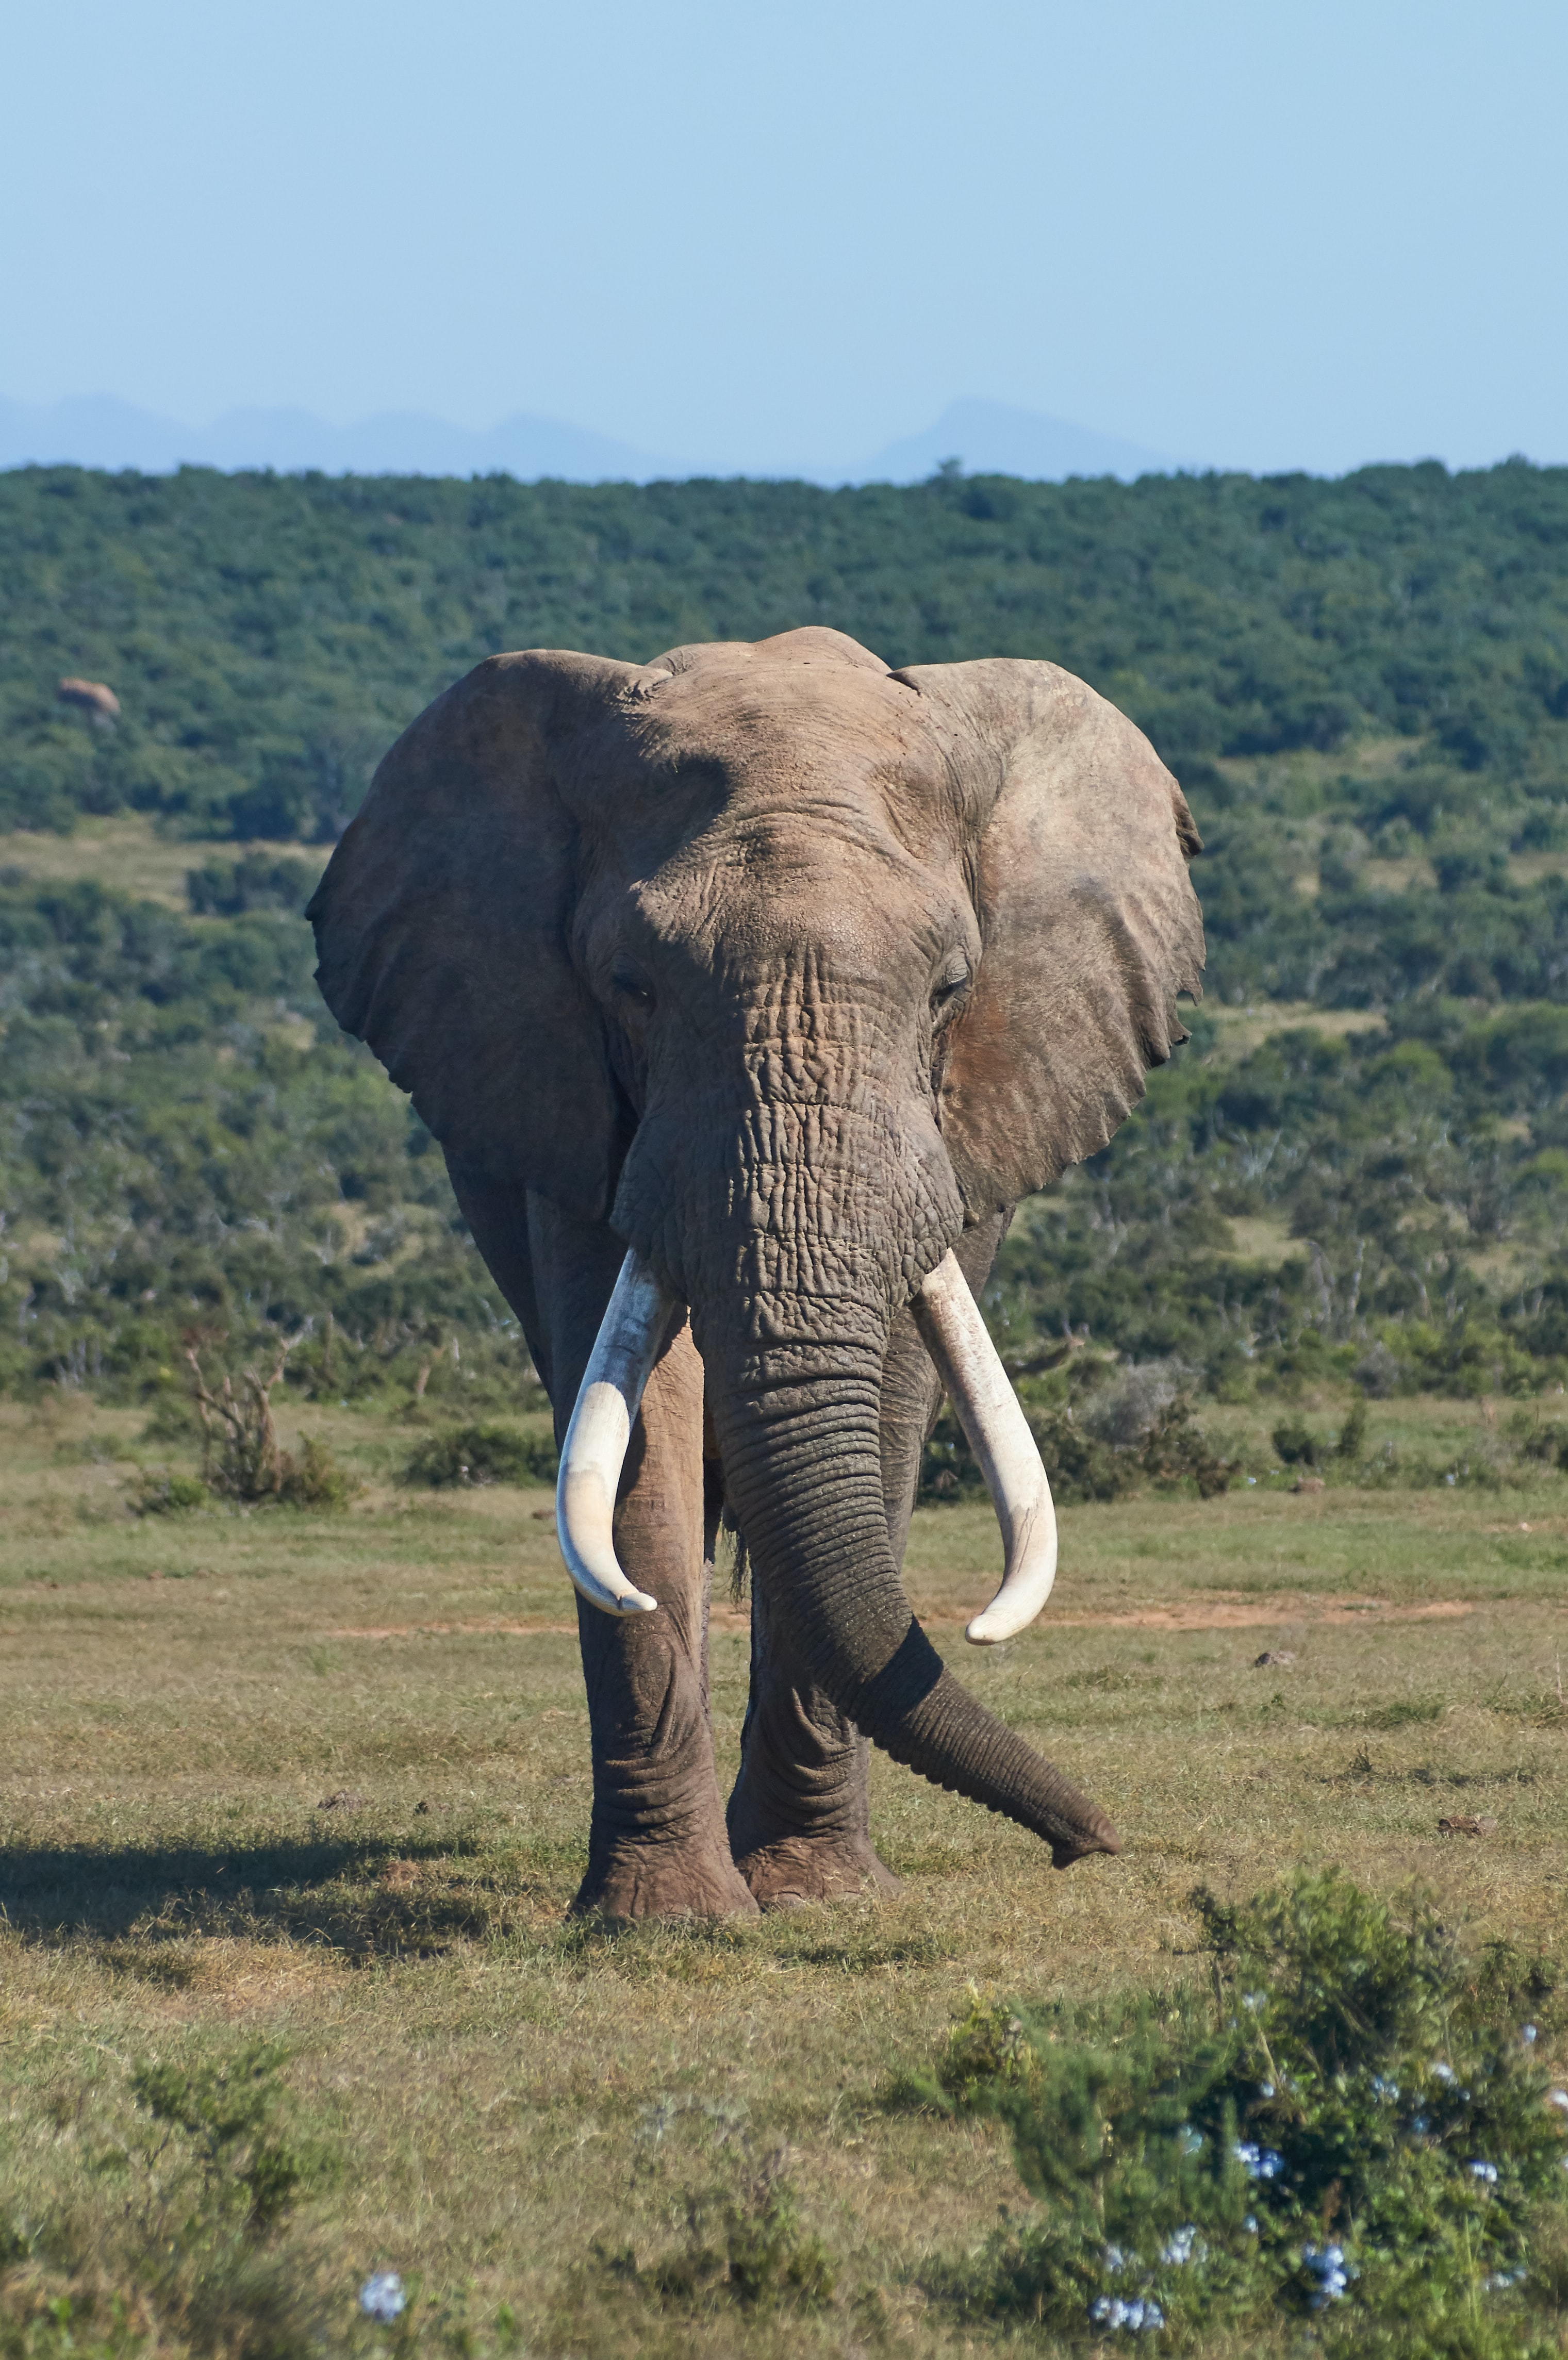
\includegraphics[width=\textwidth]{elephant.jpg}
\end{column}

\begin{column}{5cm}

\[
\text{Druck} = \frac{\text{Kraft}}{\text{Fläche}}
\]

$\,$\\[0.5cm]

\begin{center}
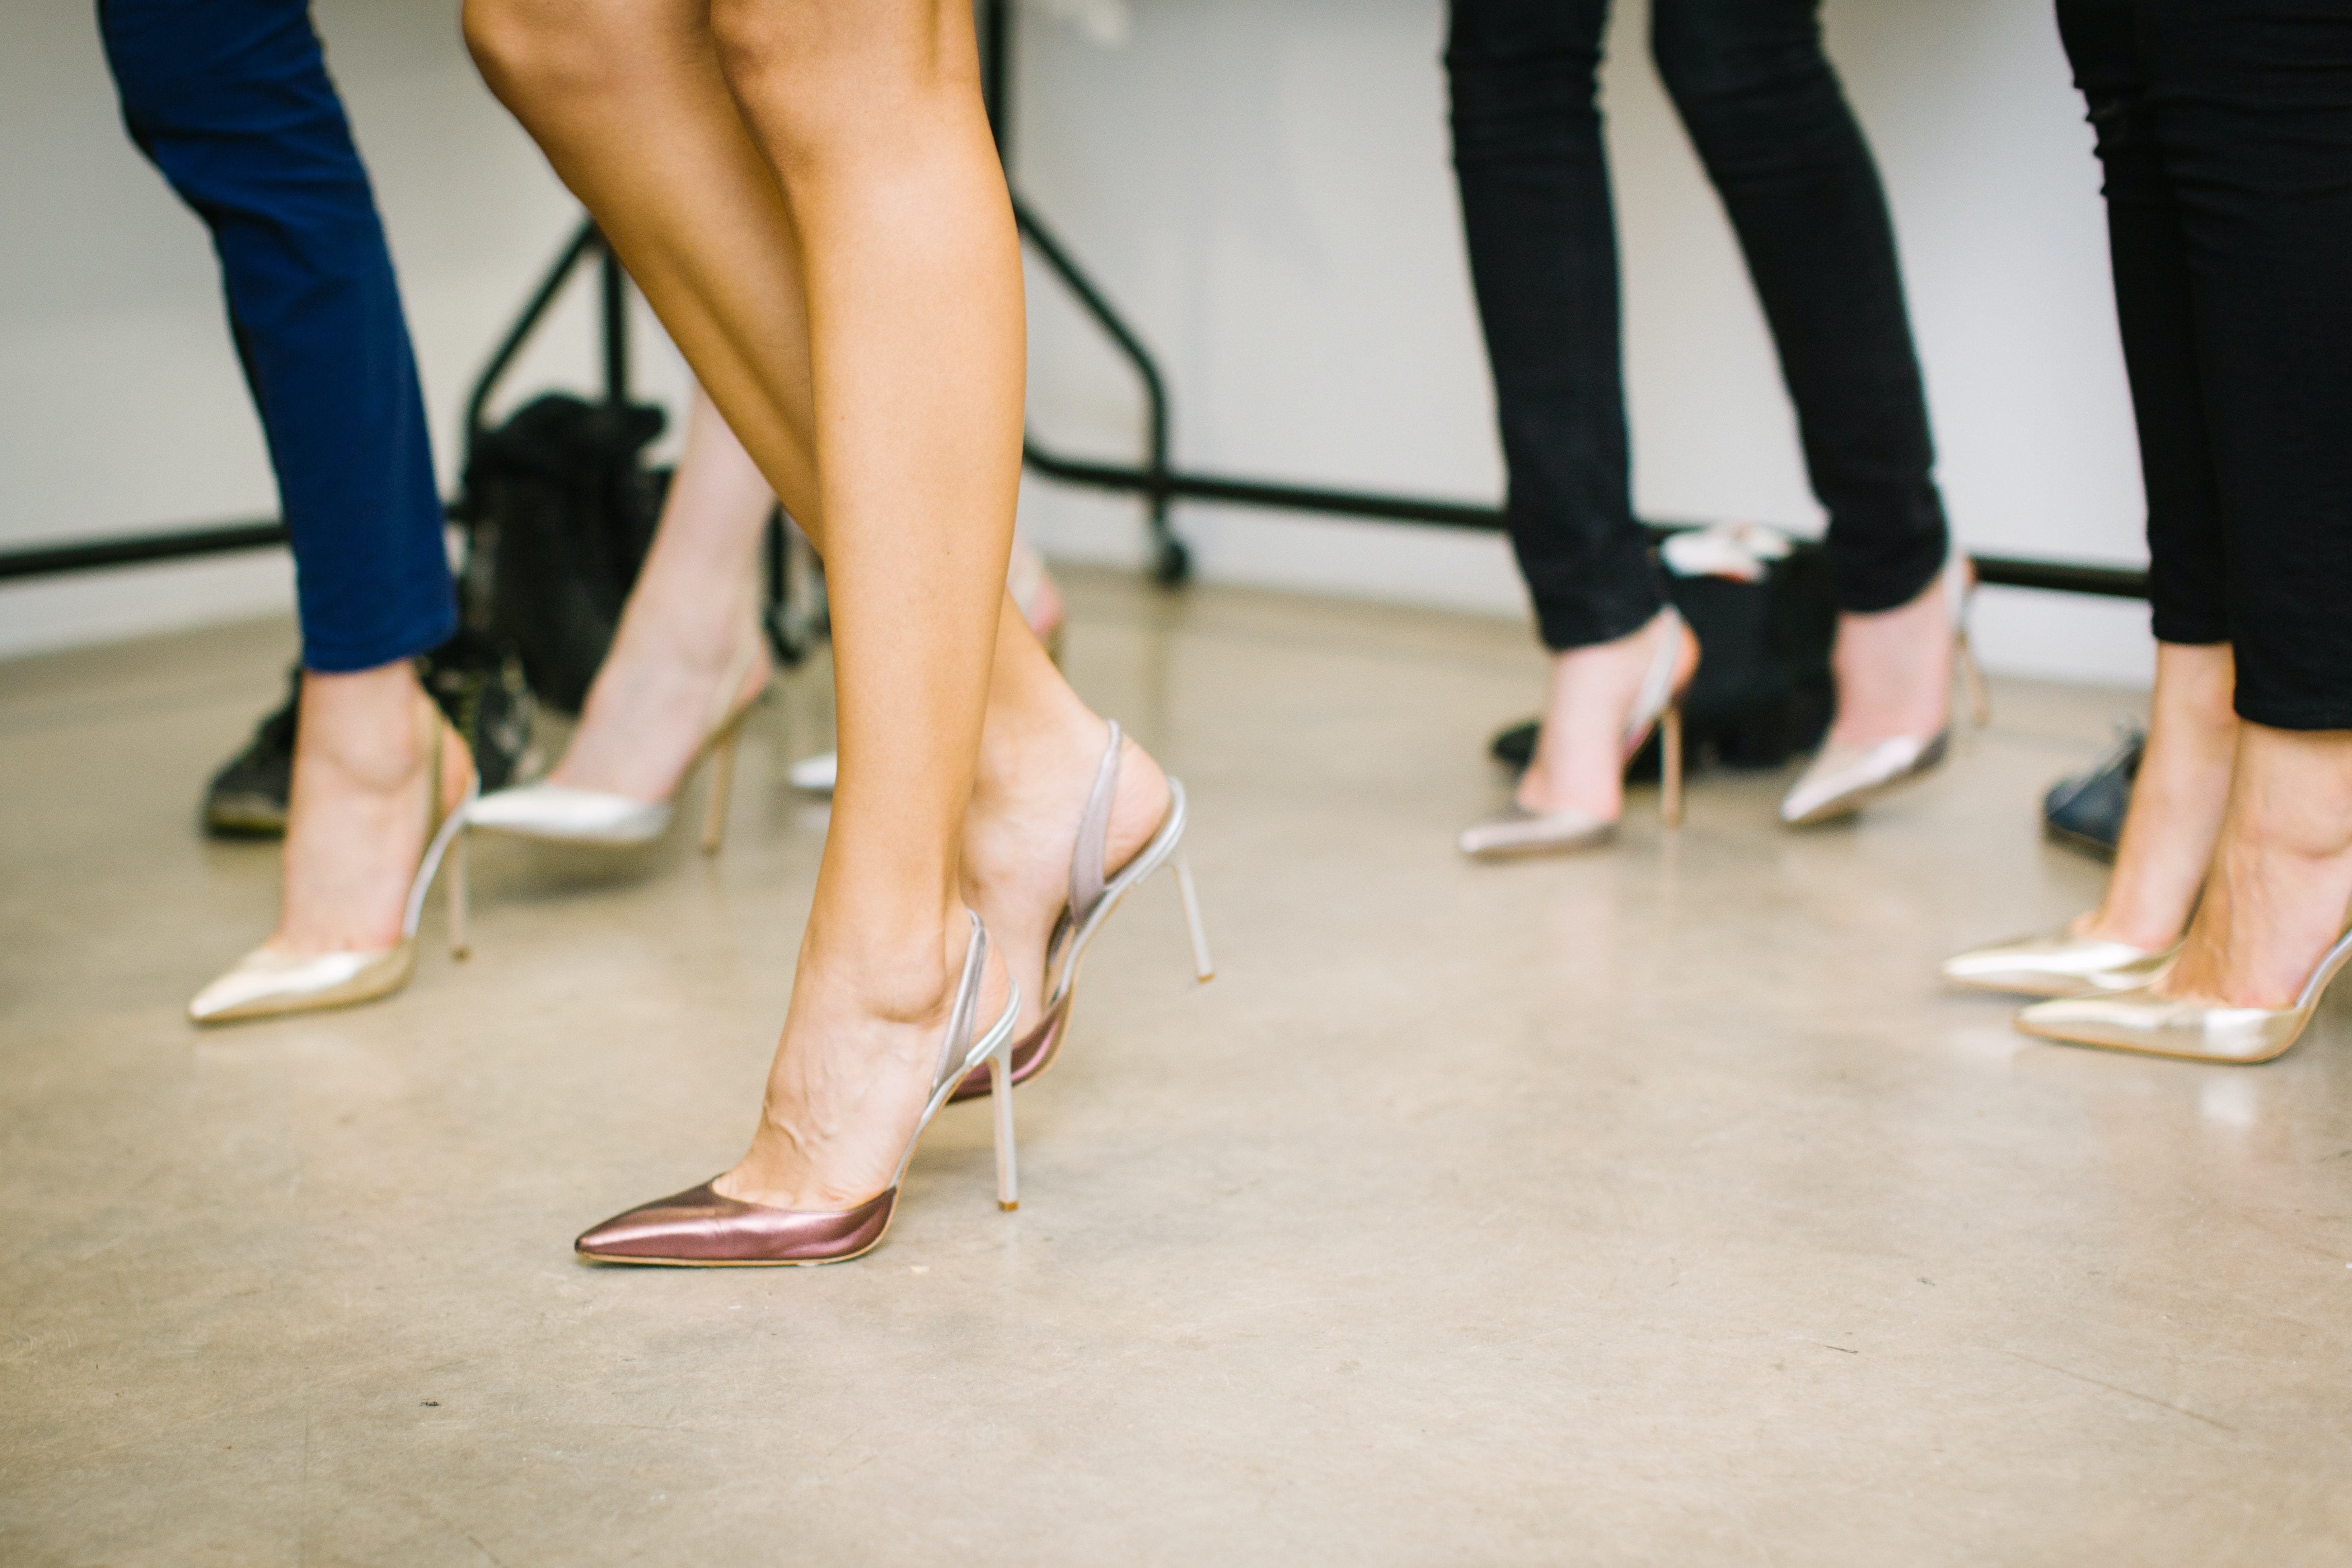
\includegraphics[width=\textwidth]{stiletto.jpg}
\end{center}

\end{column}

\end{columns}
\end{frame}


% Stempeldruck pop quiz: Was passiert, wenn man drückt?
\begin{frame}
\frametitle{Was passiert?}

\begin{columns}[c]

\begin{column}{5cm}
\begin{center}
\includegraphics<1>[width=0.8\textwidth]{stempeldruck_fluessigkeit.png}
\includegraphics<2>[width=0.8\textwidth]{stempeldruck_fluessigkeit_2.png}
\end{center}
\end{column}

\begin{column}{5cm}
\begin{center}
\includegraphics<1>[width=0.8\textwidth]{stempeldruck_gas.png}
\includegraphics<2>[width=0.8\textwidth]{stempeldruck_gas_2.png}
\end{center}
\end{column}



\end{columns}

\end{frame}

%% Eigenschatften von Flüssigkeiten und Gase erklären - kompressible oder nicht
\begin{frame}
\frametitle{Gase sind kompressibel, Flüssigkeiten nicht}

\begin{columns}[c]

\begin{column}{5cm}
\begin{center}
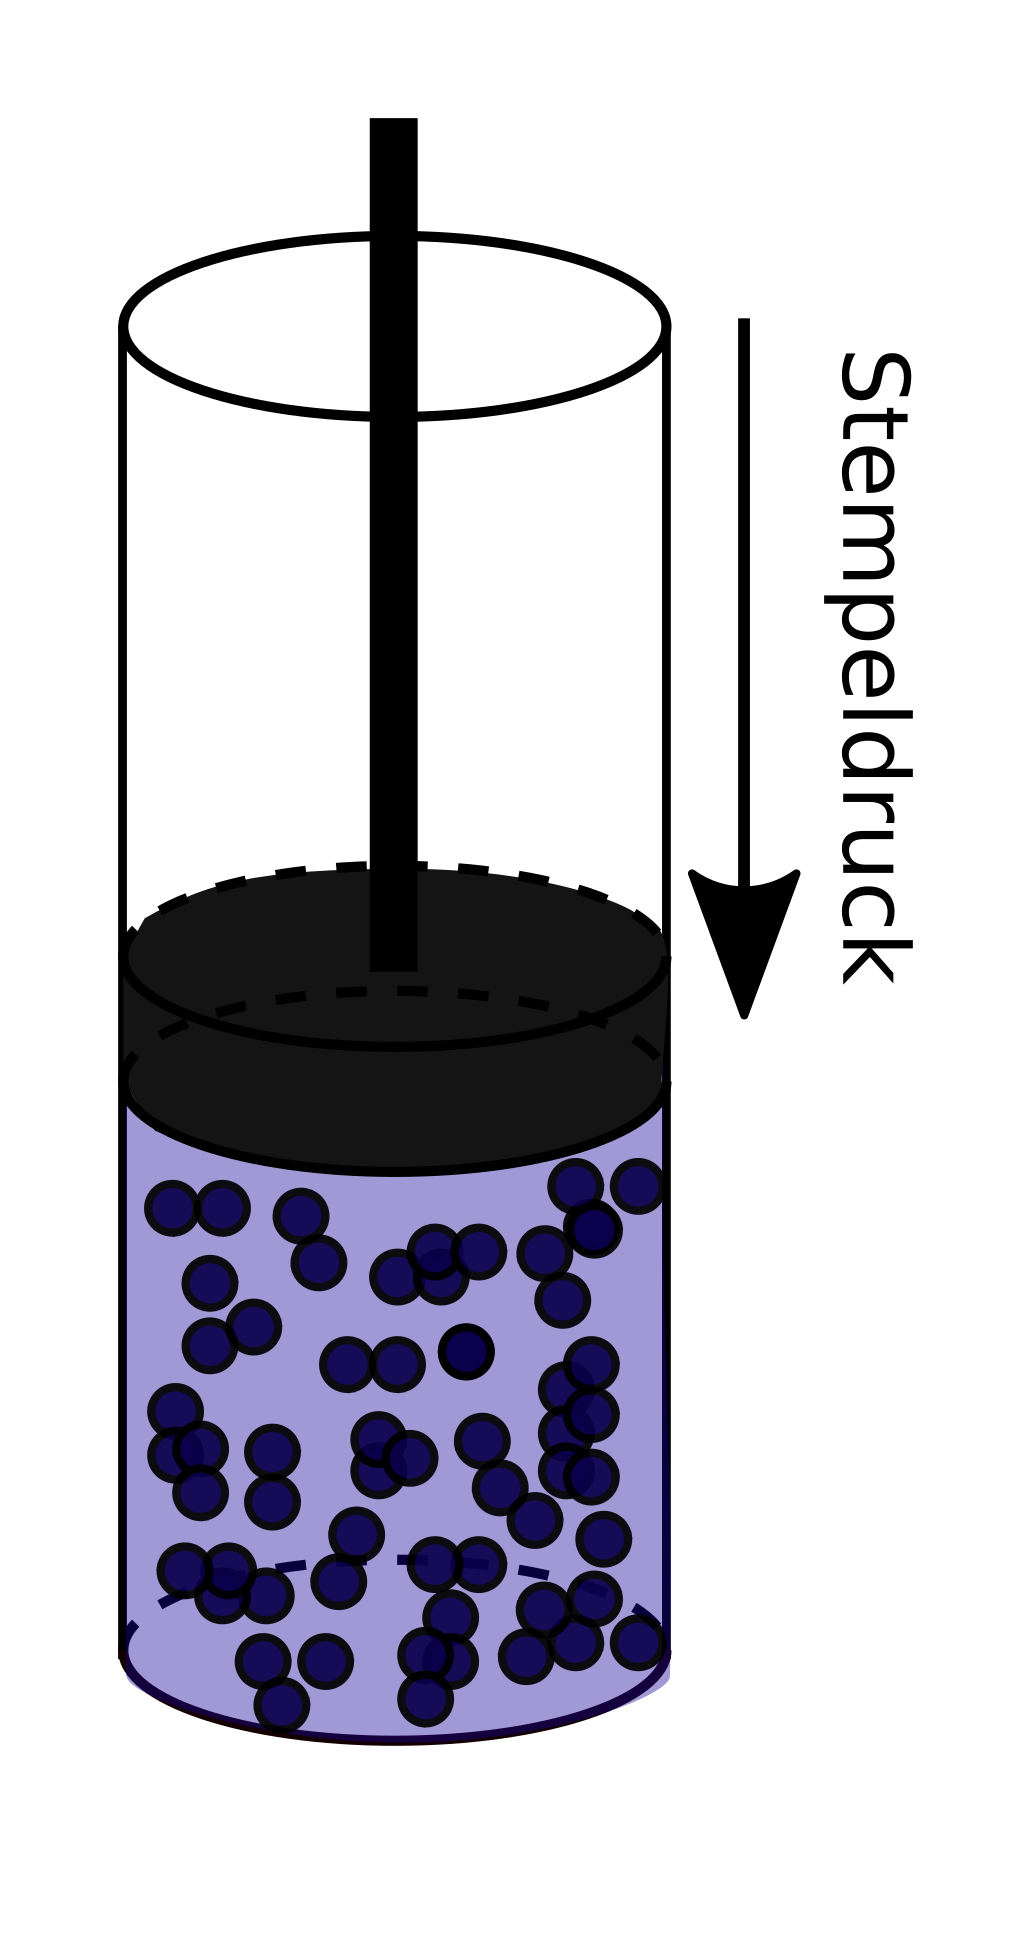
\includegraphics[width=0.8\textwidth]{stempeldruck_fluessigkeit_2.png}
\end{center}
\end{column}

\begin{column}{5cm}
\begin{center}
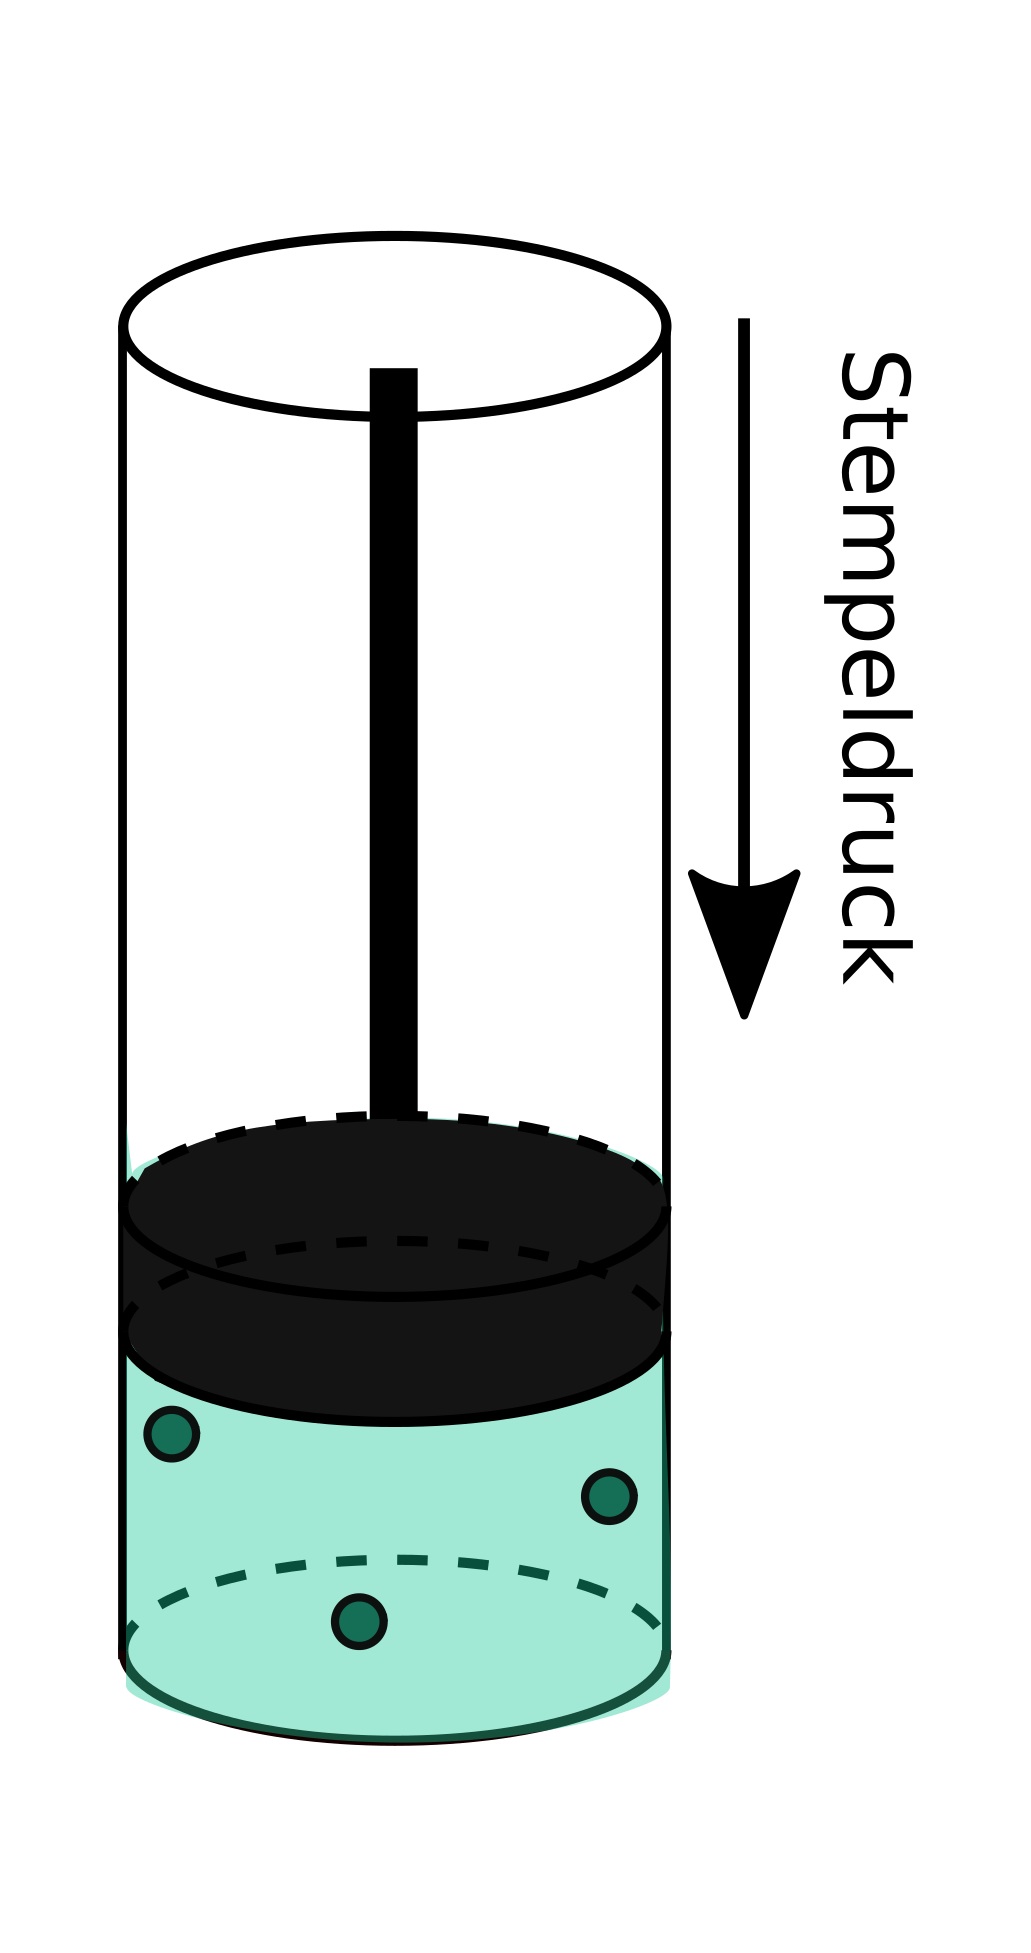
\includegraphics[width=0.8\textwidth]{stempeldruck_gas_3.png}
\end{center}
\end{column}

\end{columns}


\end{frame}


%% Herz als Pumpe
\begin{frame}
\frametitle{Flüssigkeiten können durch Druck bewegt werden}

\begin{columns}[c]

\begin{column}{5cm}
\begin{center}
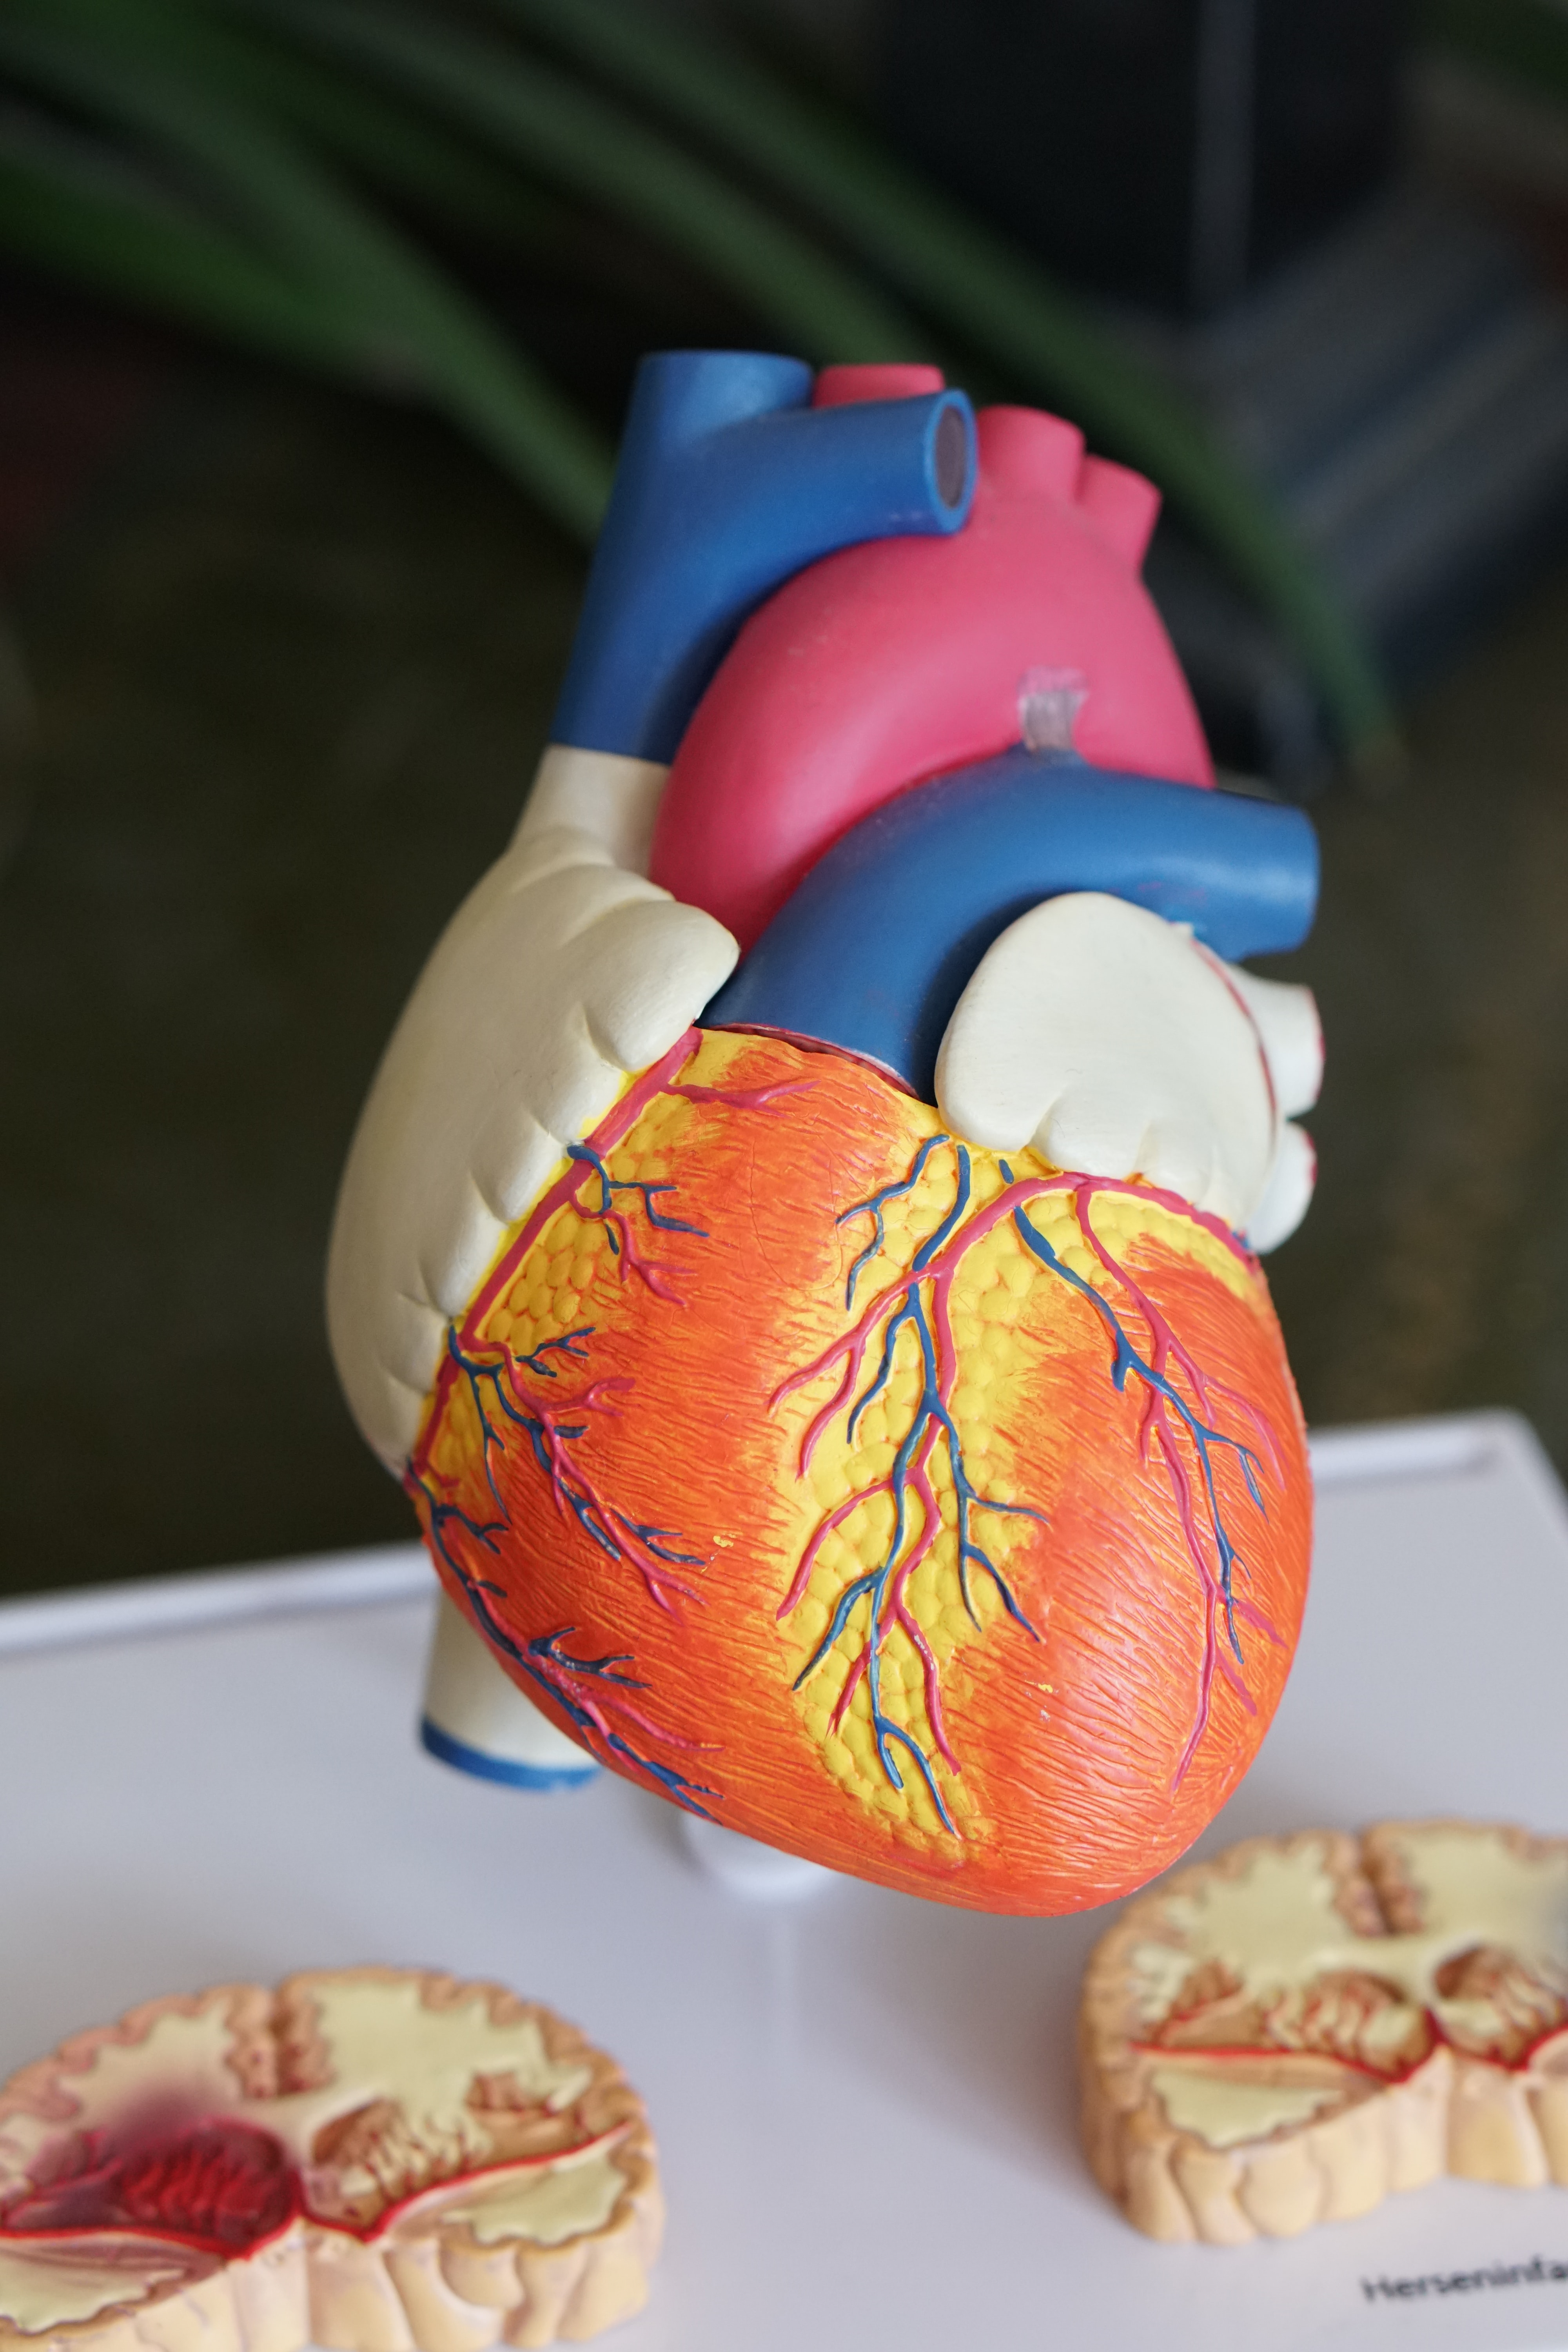
\includegraphics[width=\textwidth]{heart.jpg}
\end{center}
\end{column}

\begin{column}{5cm}
\begin{block}{Beispiel}
Das Herz funktioniert als Pumpe, die Blut durch den Kreislauf bewegt
\end{block}
\end{column}

\end{columns}


\end{frame}



%% Wasserdruck, Auftrieb, Abhängigkeit von Tiefe
\begin{frame}
\makebox[\linewidth]{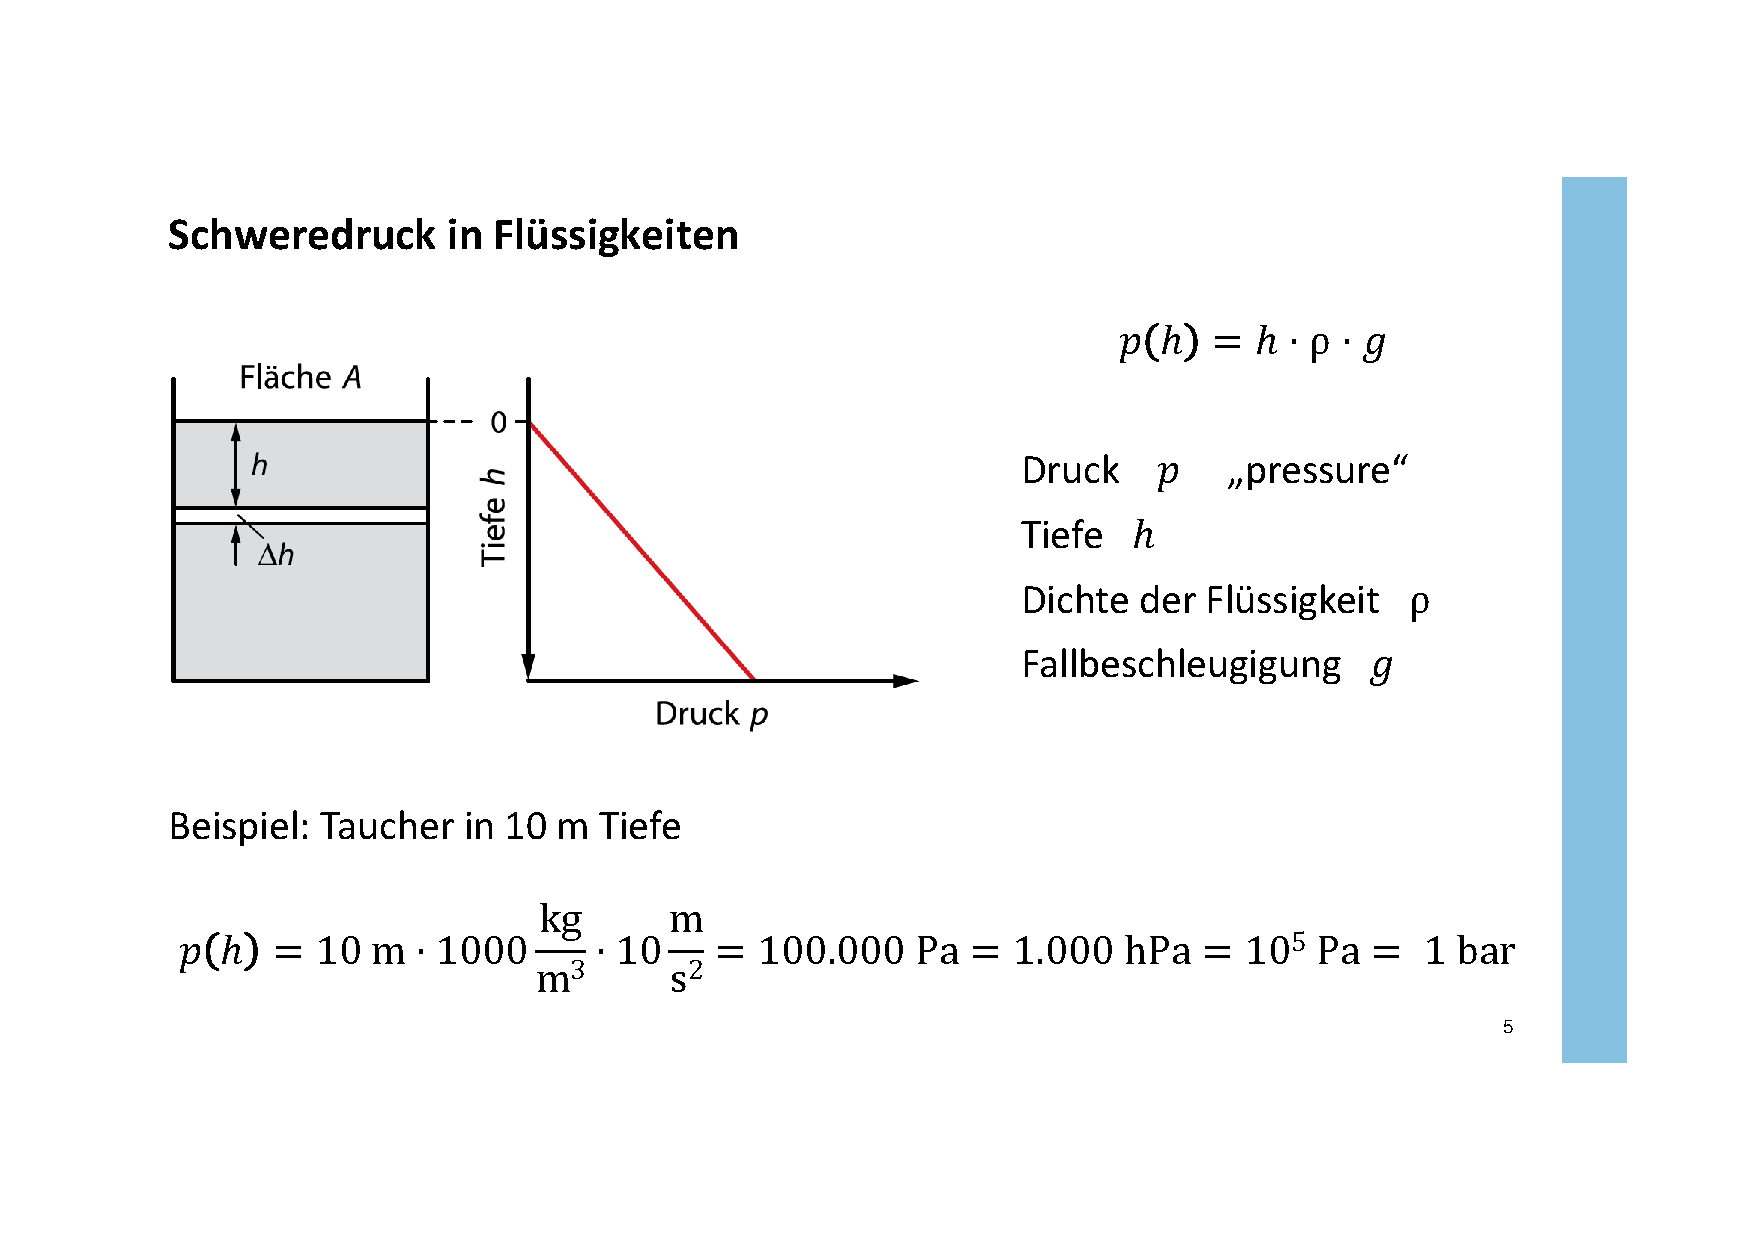
\includegraphics[width=\textwidth]{Walter_Druck_Schweredruck_Fluessigkeiten.pdf}}
\end{frame}


\begin{frame}
\makebox[\linewidth]{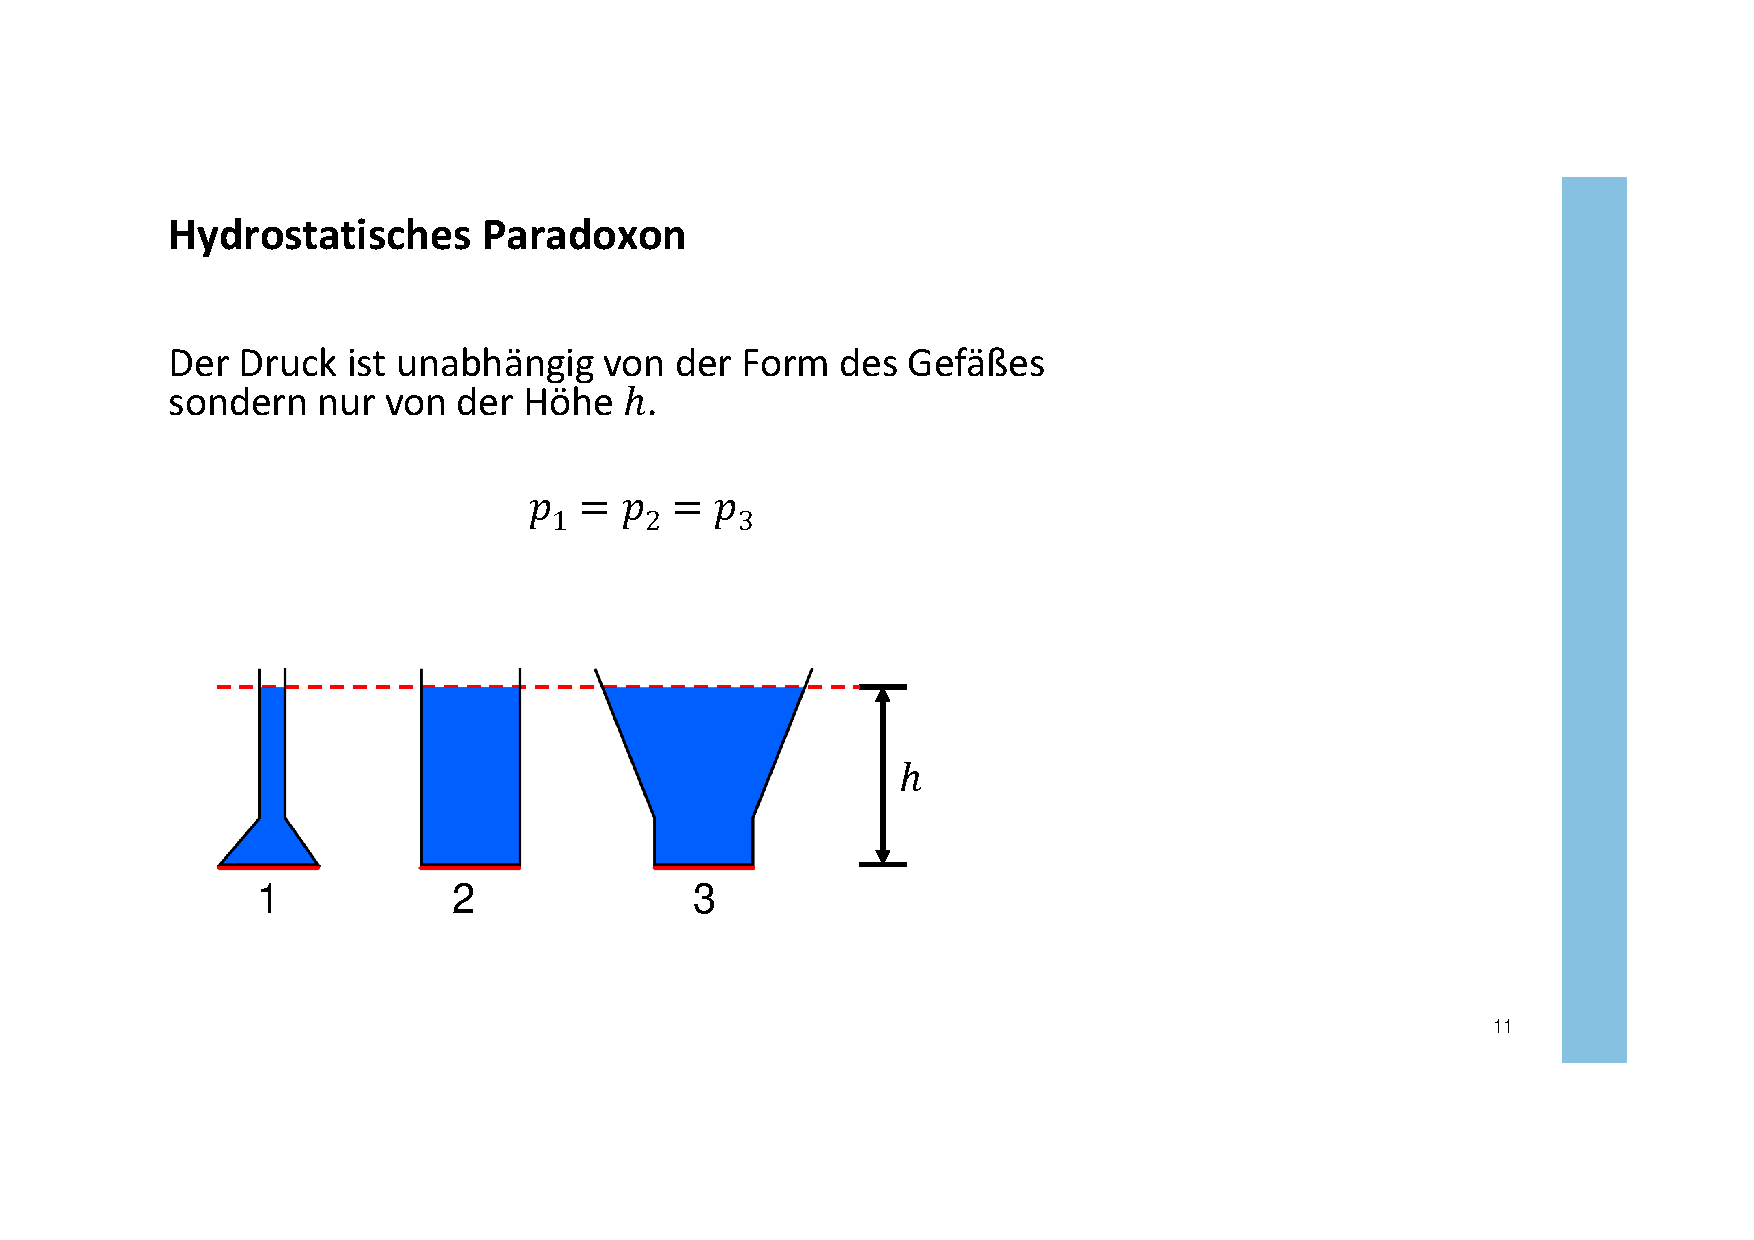
\includegraphics[width=\textwidth]{Walter_Druck_Hydrostatisches_Paradoxon.pdf}}
\end{frame}


%% Auftrieb

\begin{frame}
\makebox[\linewidth]{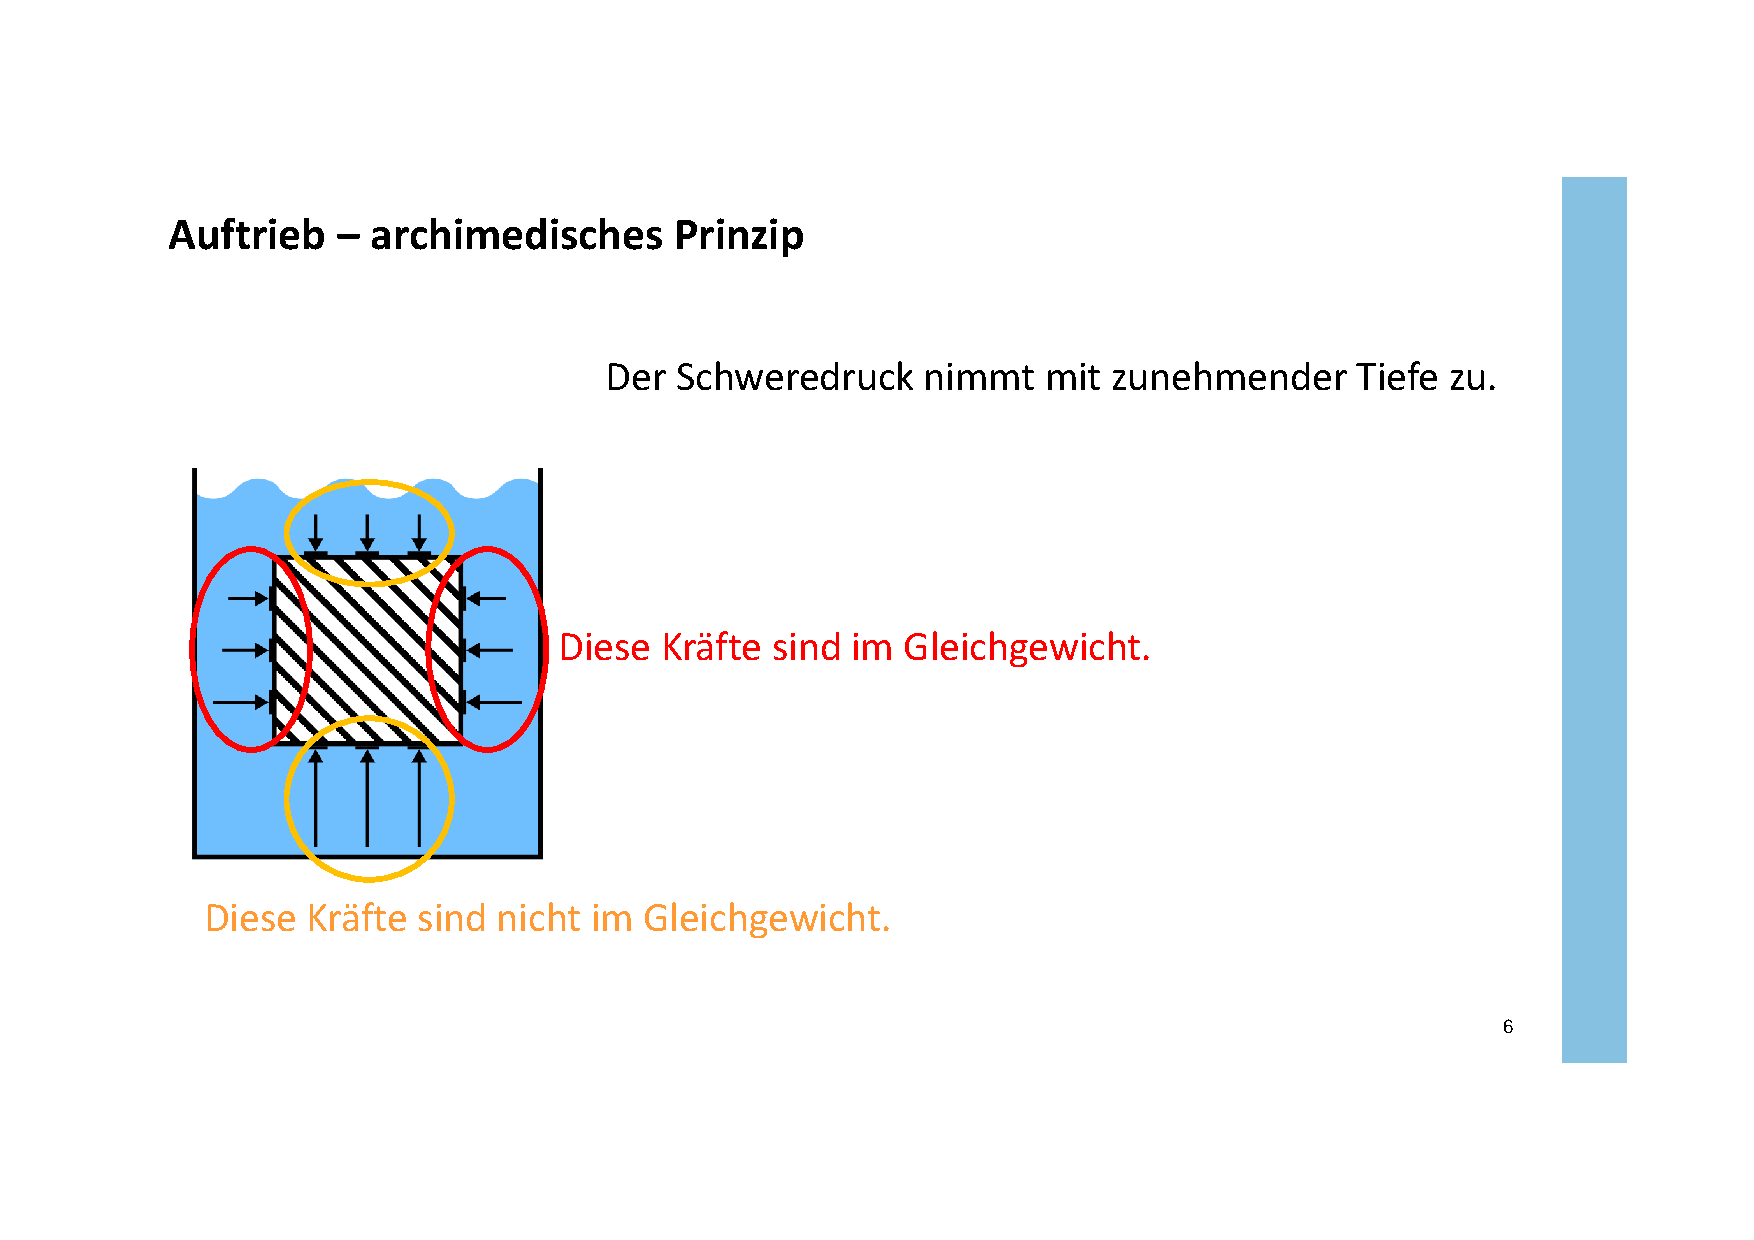
\includegraphics[width=\textwidth]{Walter_Druck_Auftrieb1.pdf}}
\end{frame}

\begin{frame}
\makebox[\linewidth]{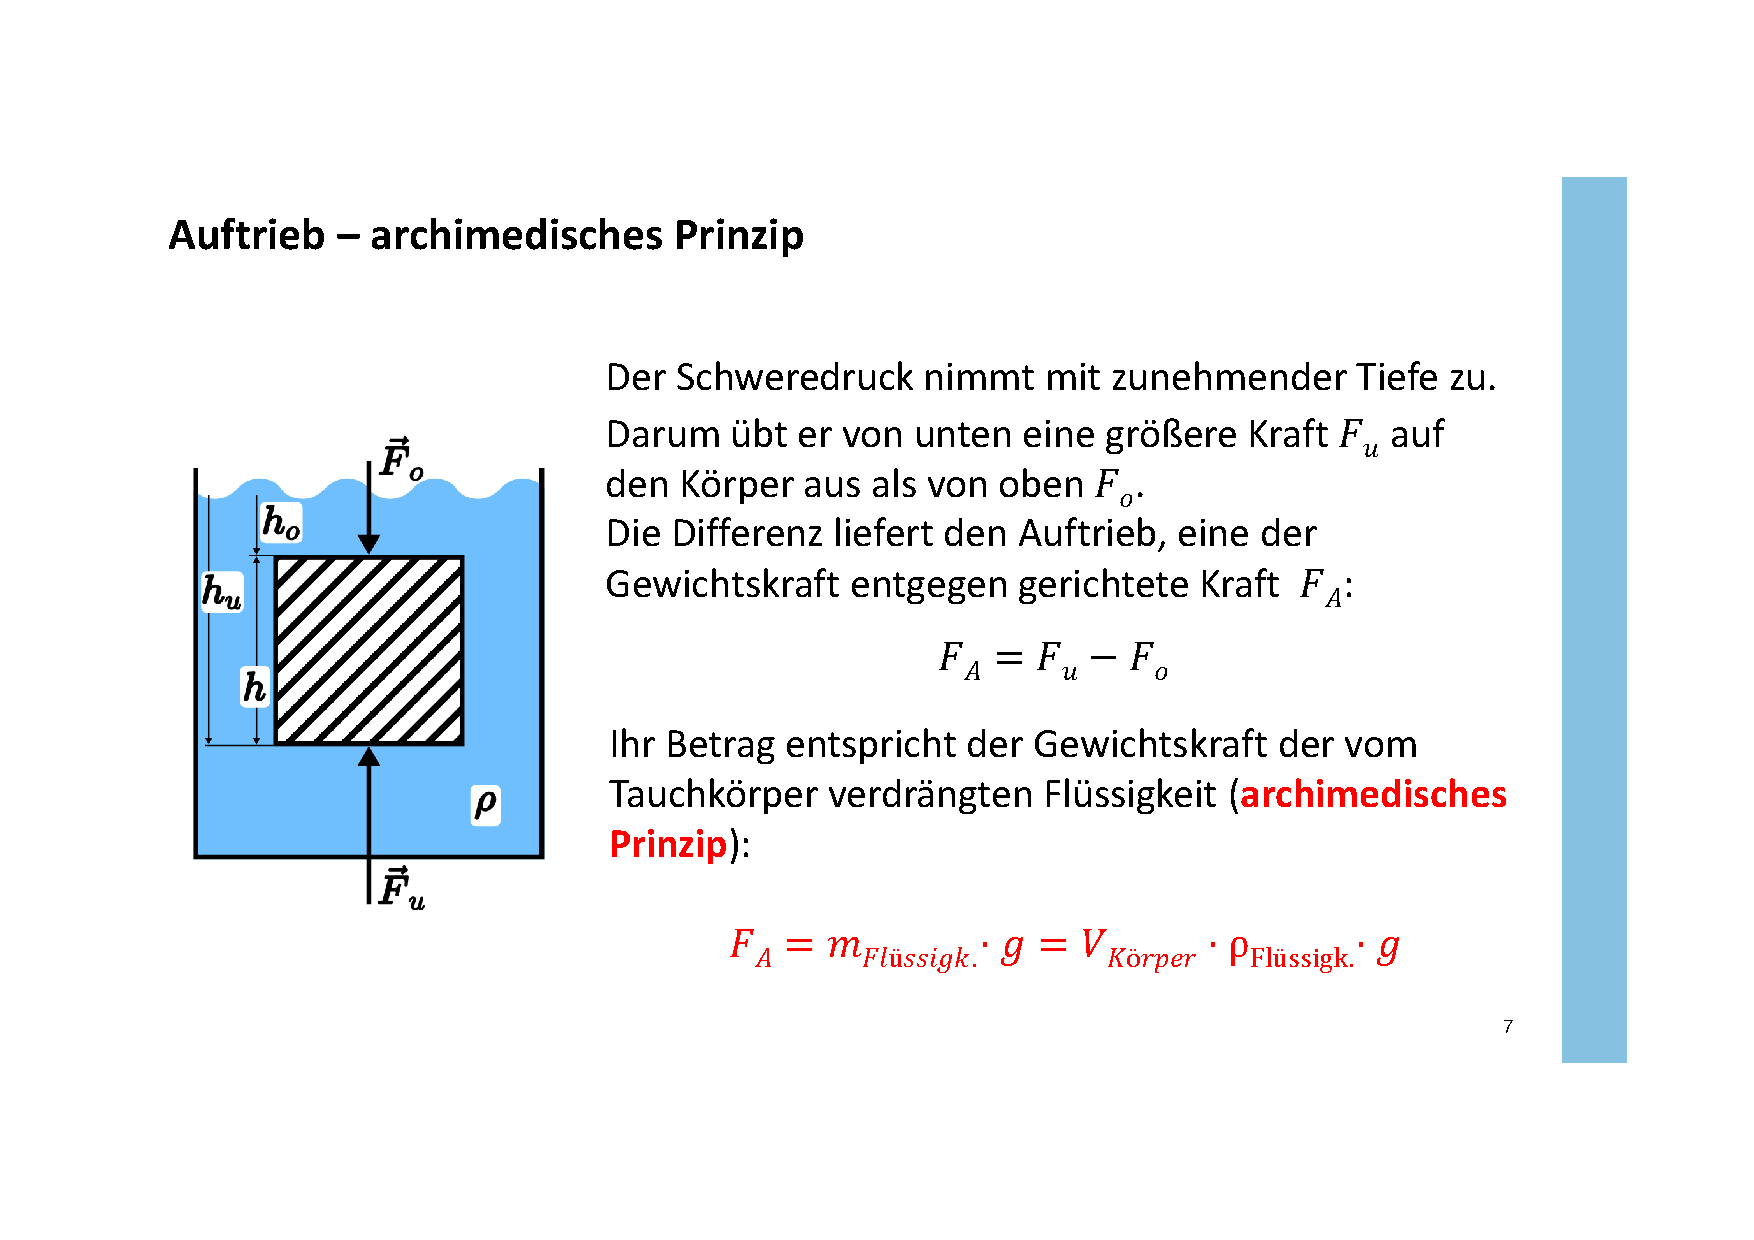
\includegraphics[width=\textwidth]{Walter_Druck_Auftrieb2.pdf}}
\end{frame}

\begin{frame}
\makebox[\linewidth]{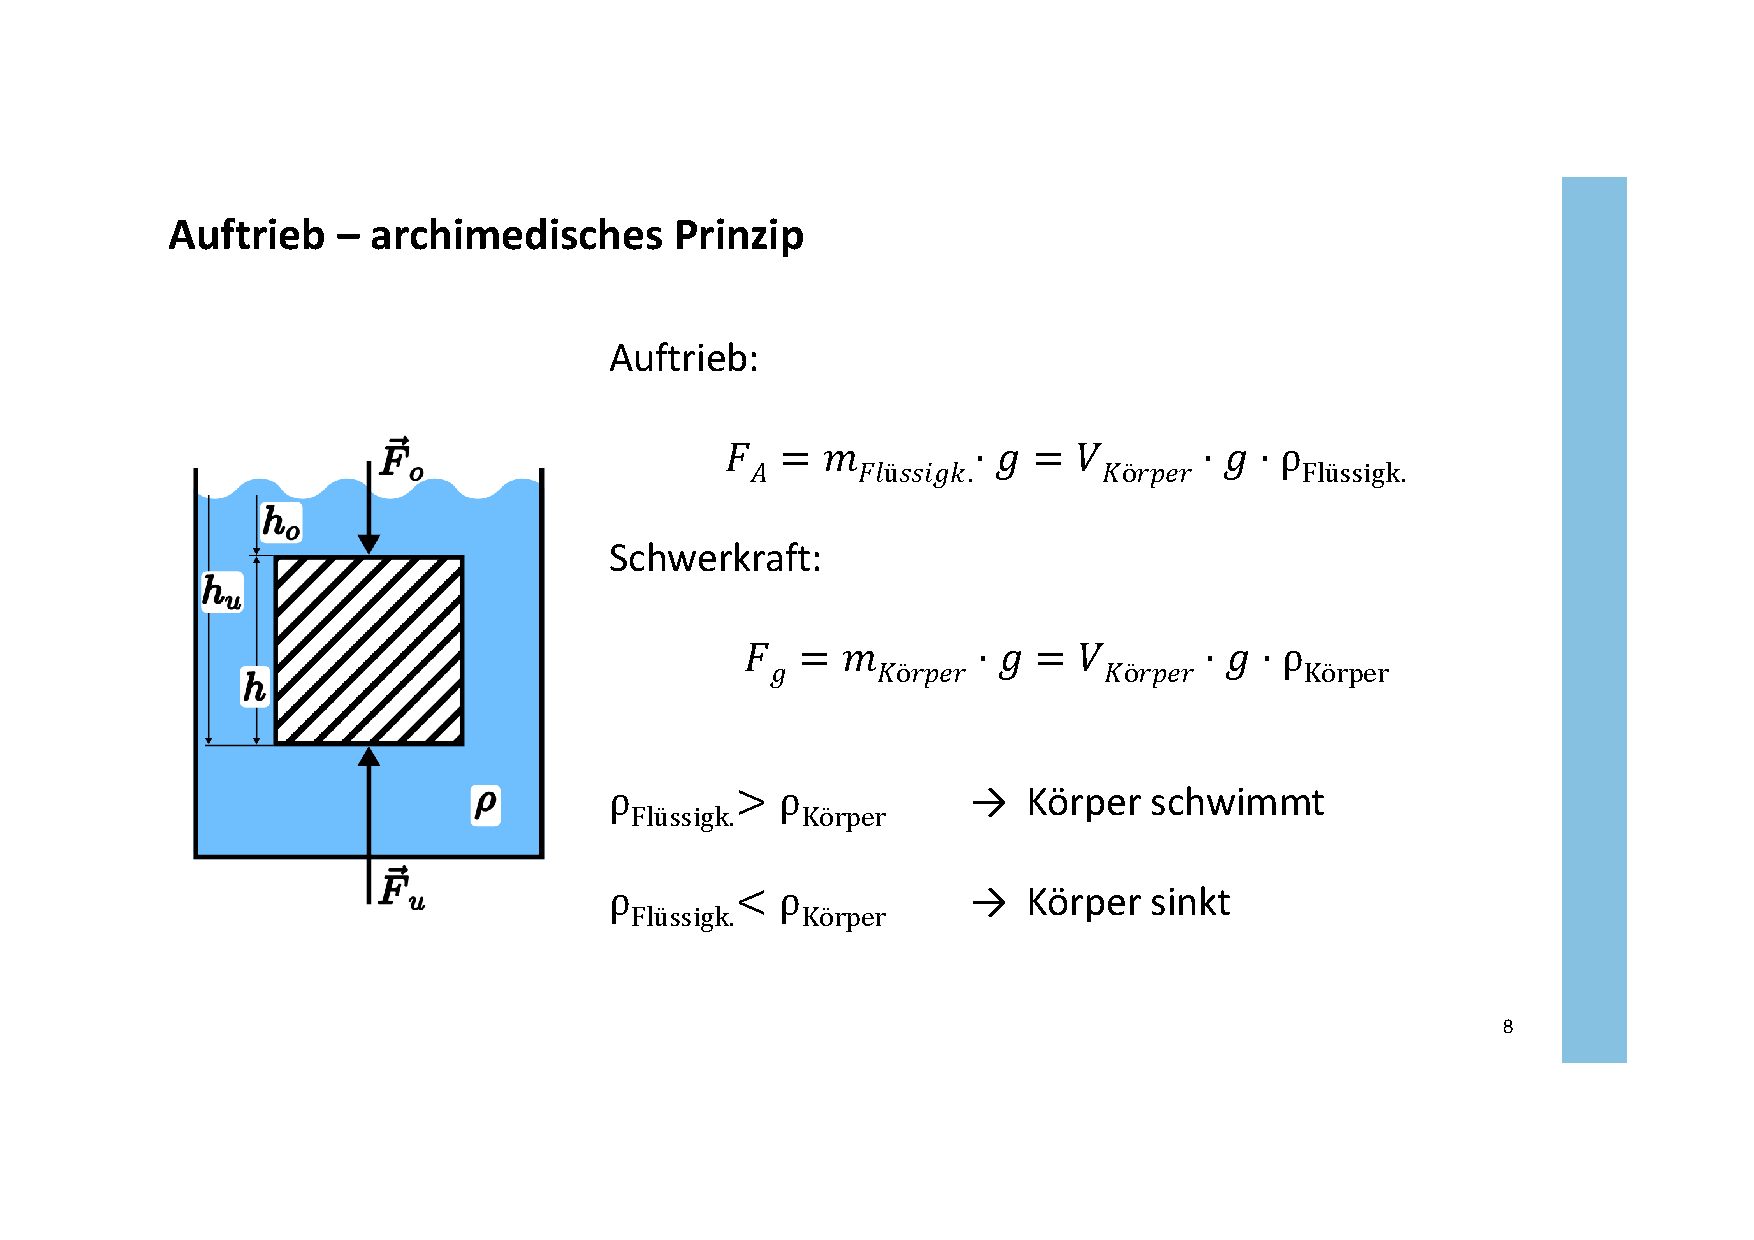
\includegraphics[width=\textwidth]{Walter_Druck_Auftrieb3.pdf}}
\end{frame}



%% Luftdruck, Abhängigkeit von Höhe
\begin{frame}
\frametitle{Luftdruck}

Verhält sich Luftdruck im Prinzip ähnlich wie Wasserdruck? 

\begin{center}
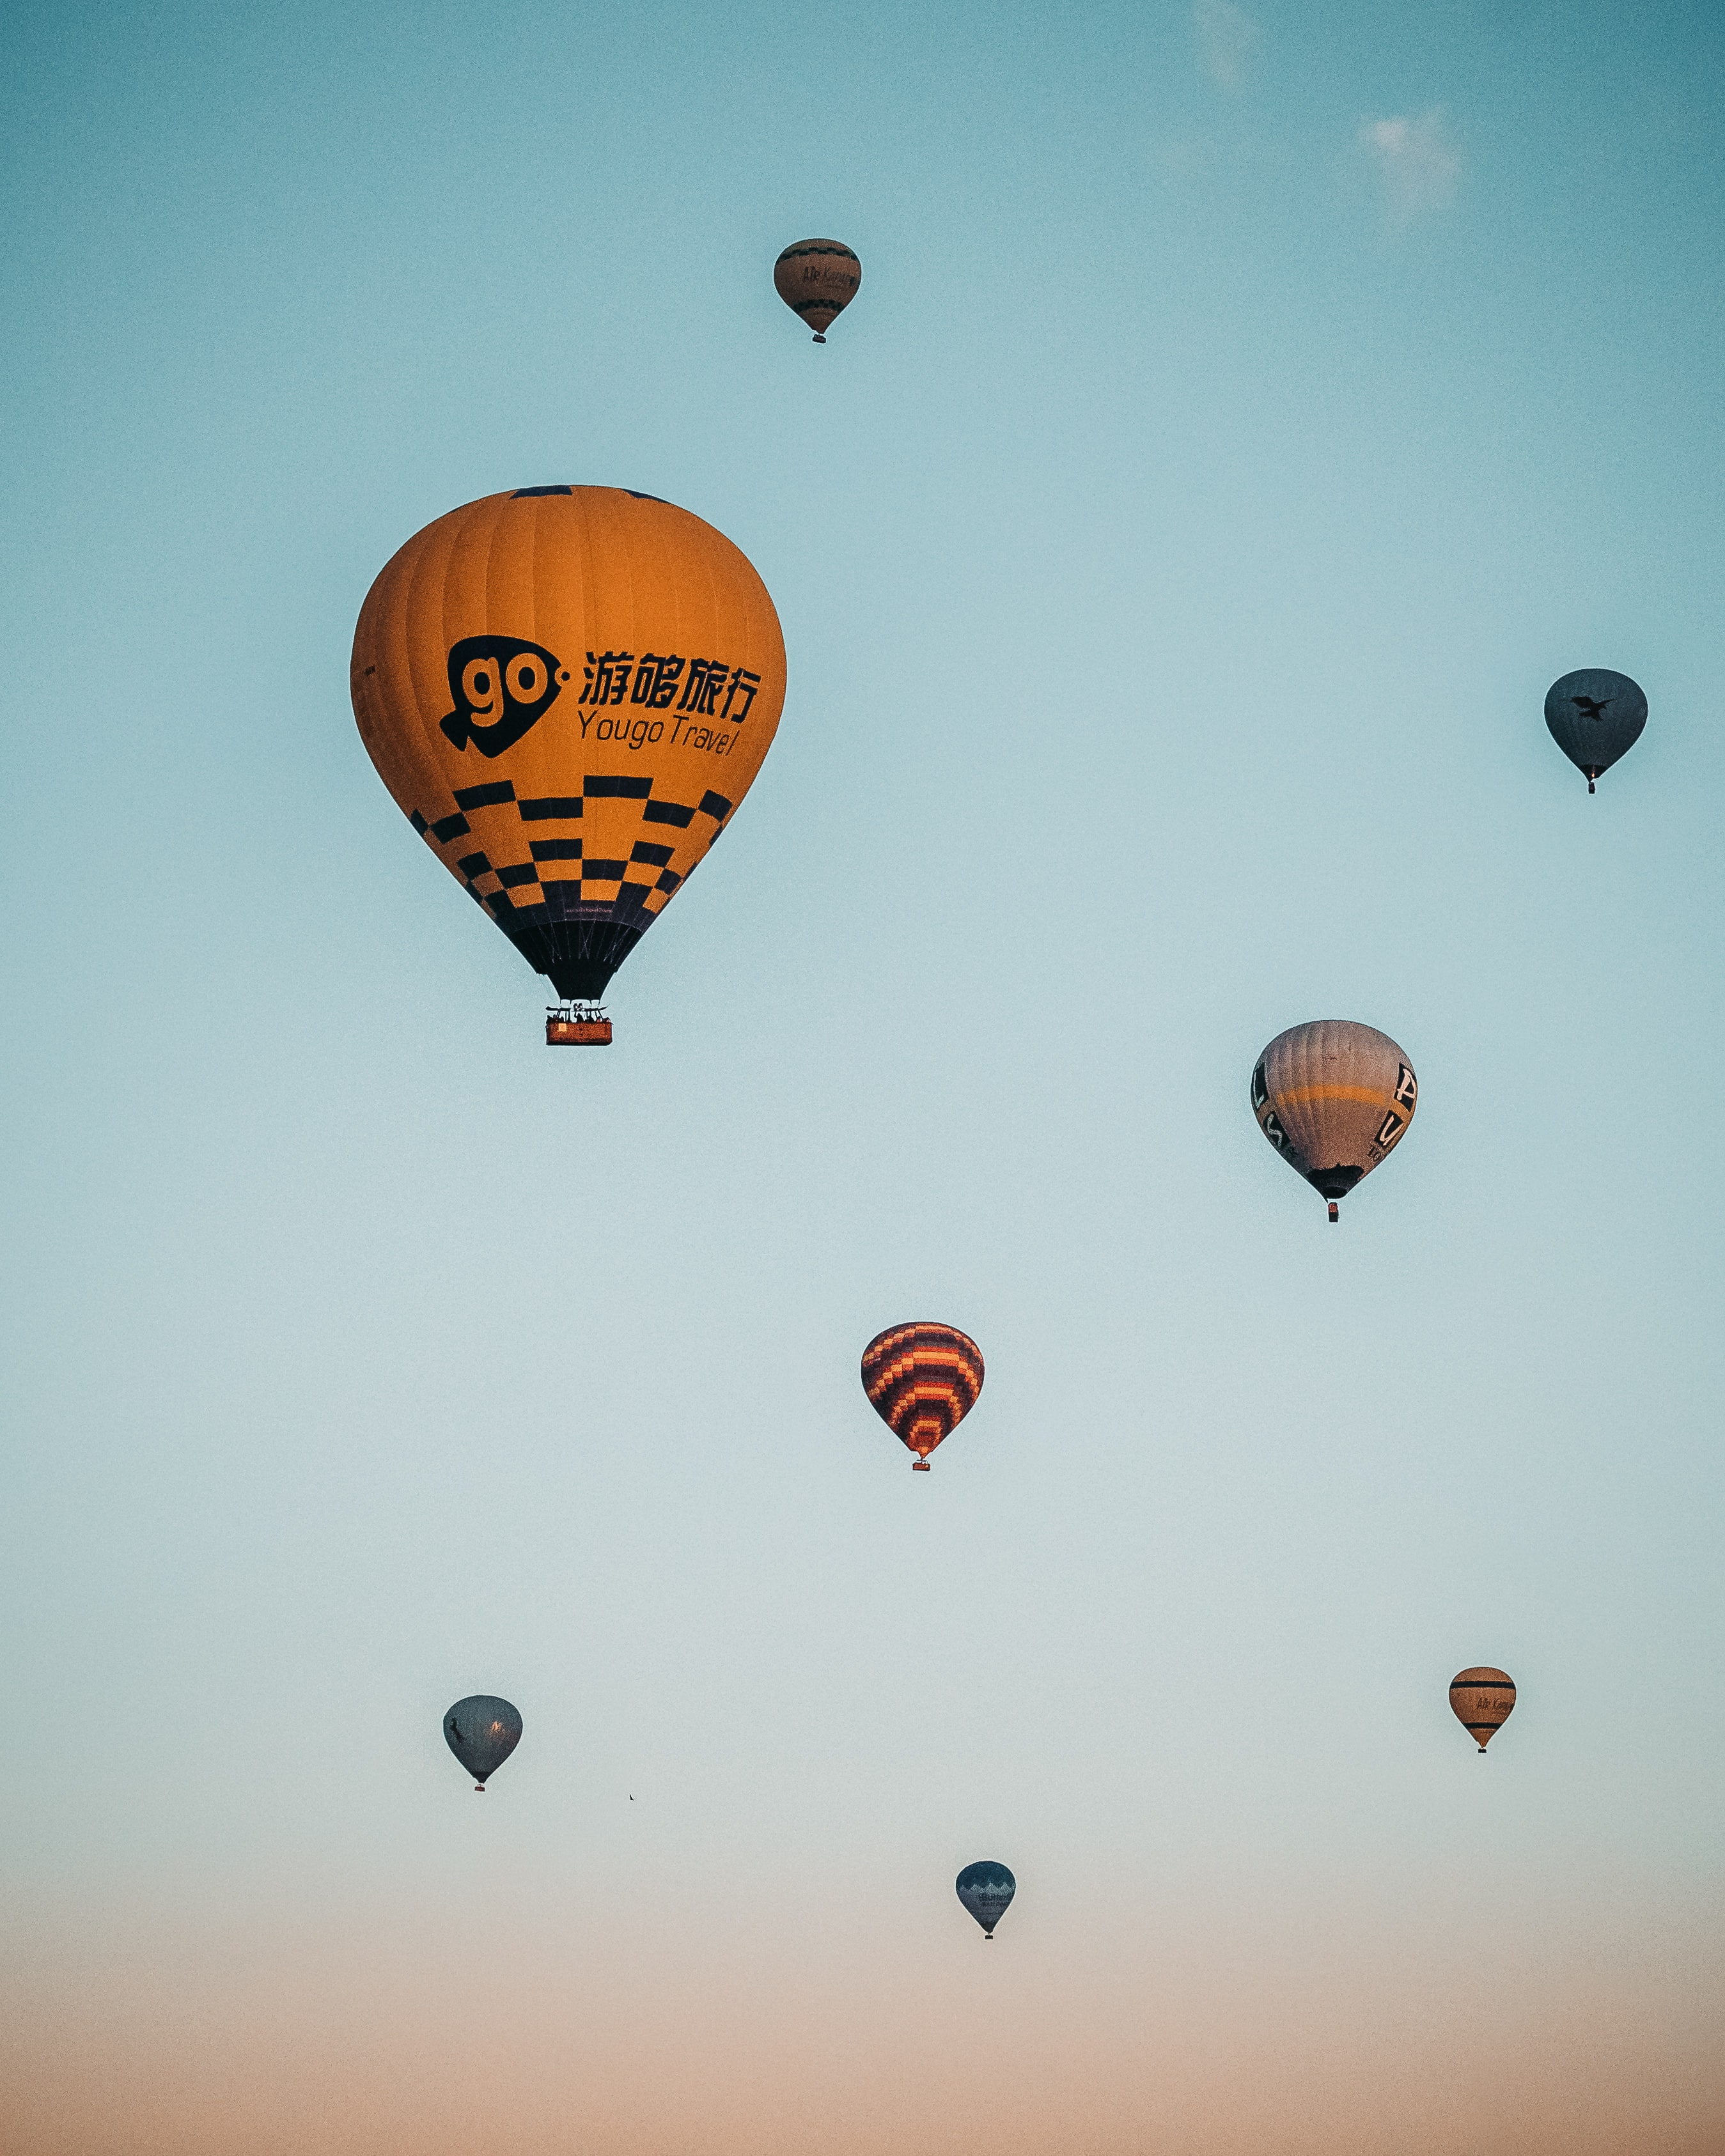
\includegraphics[width=0.5\textwidth]{hot_air_balloons.jpg}
\end{center}


\end{frame}

%% - Luftdruck an verschiedenen Orten abschätzen
\begin{frame}
\frametitle{Luftdruck}

\textcolor{theme}{Ja,} auch Luft unterliegt der Schwerkraft, und mit zunehmender Nähe zum Erdmittelpunkt nimmt der Schweredruck zu. 



\pause


\begin{columns}[c]

\begin{column}{5cm}
\textcolor{theme}{Nein,} denn im Gegensatz zu Wasser ist Luft kompressibel. Wo der Schweredruck größer ist, ist auch die Dichte größer. Mit zunehmender Höhe nimmt der Luftdruck nicht linear ab, sondern exponentiell. \\ 

\end{column}

\pause
\begin{column}{5cm}
\begin{center}
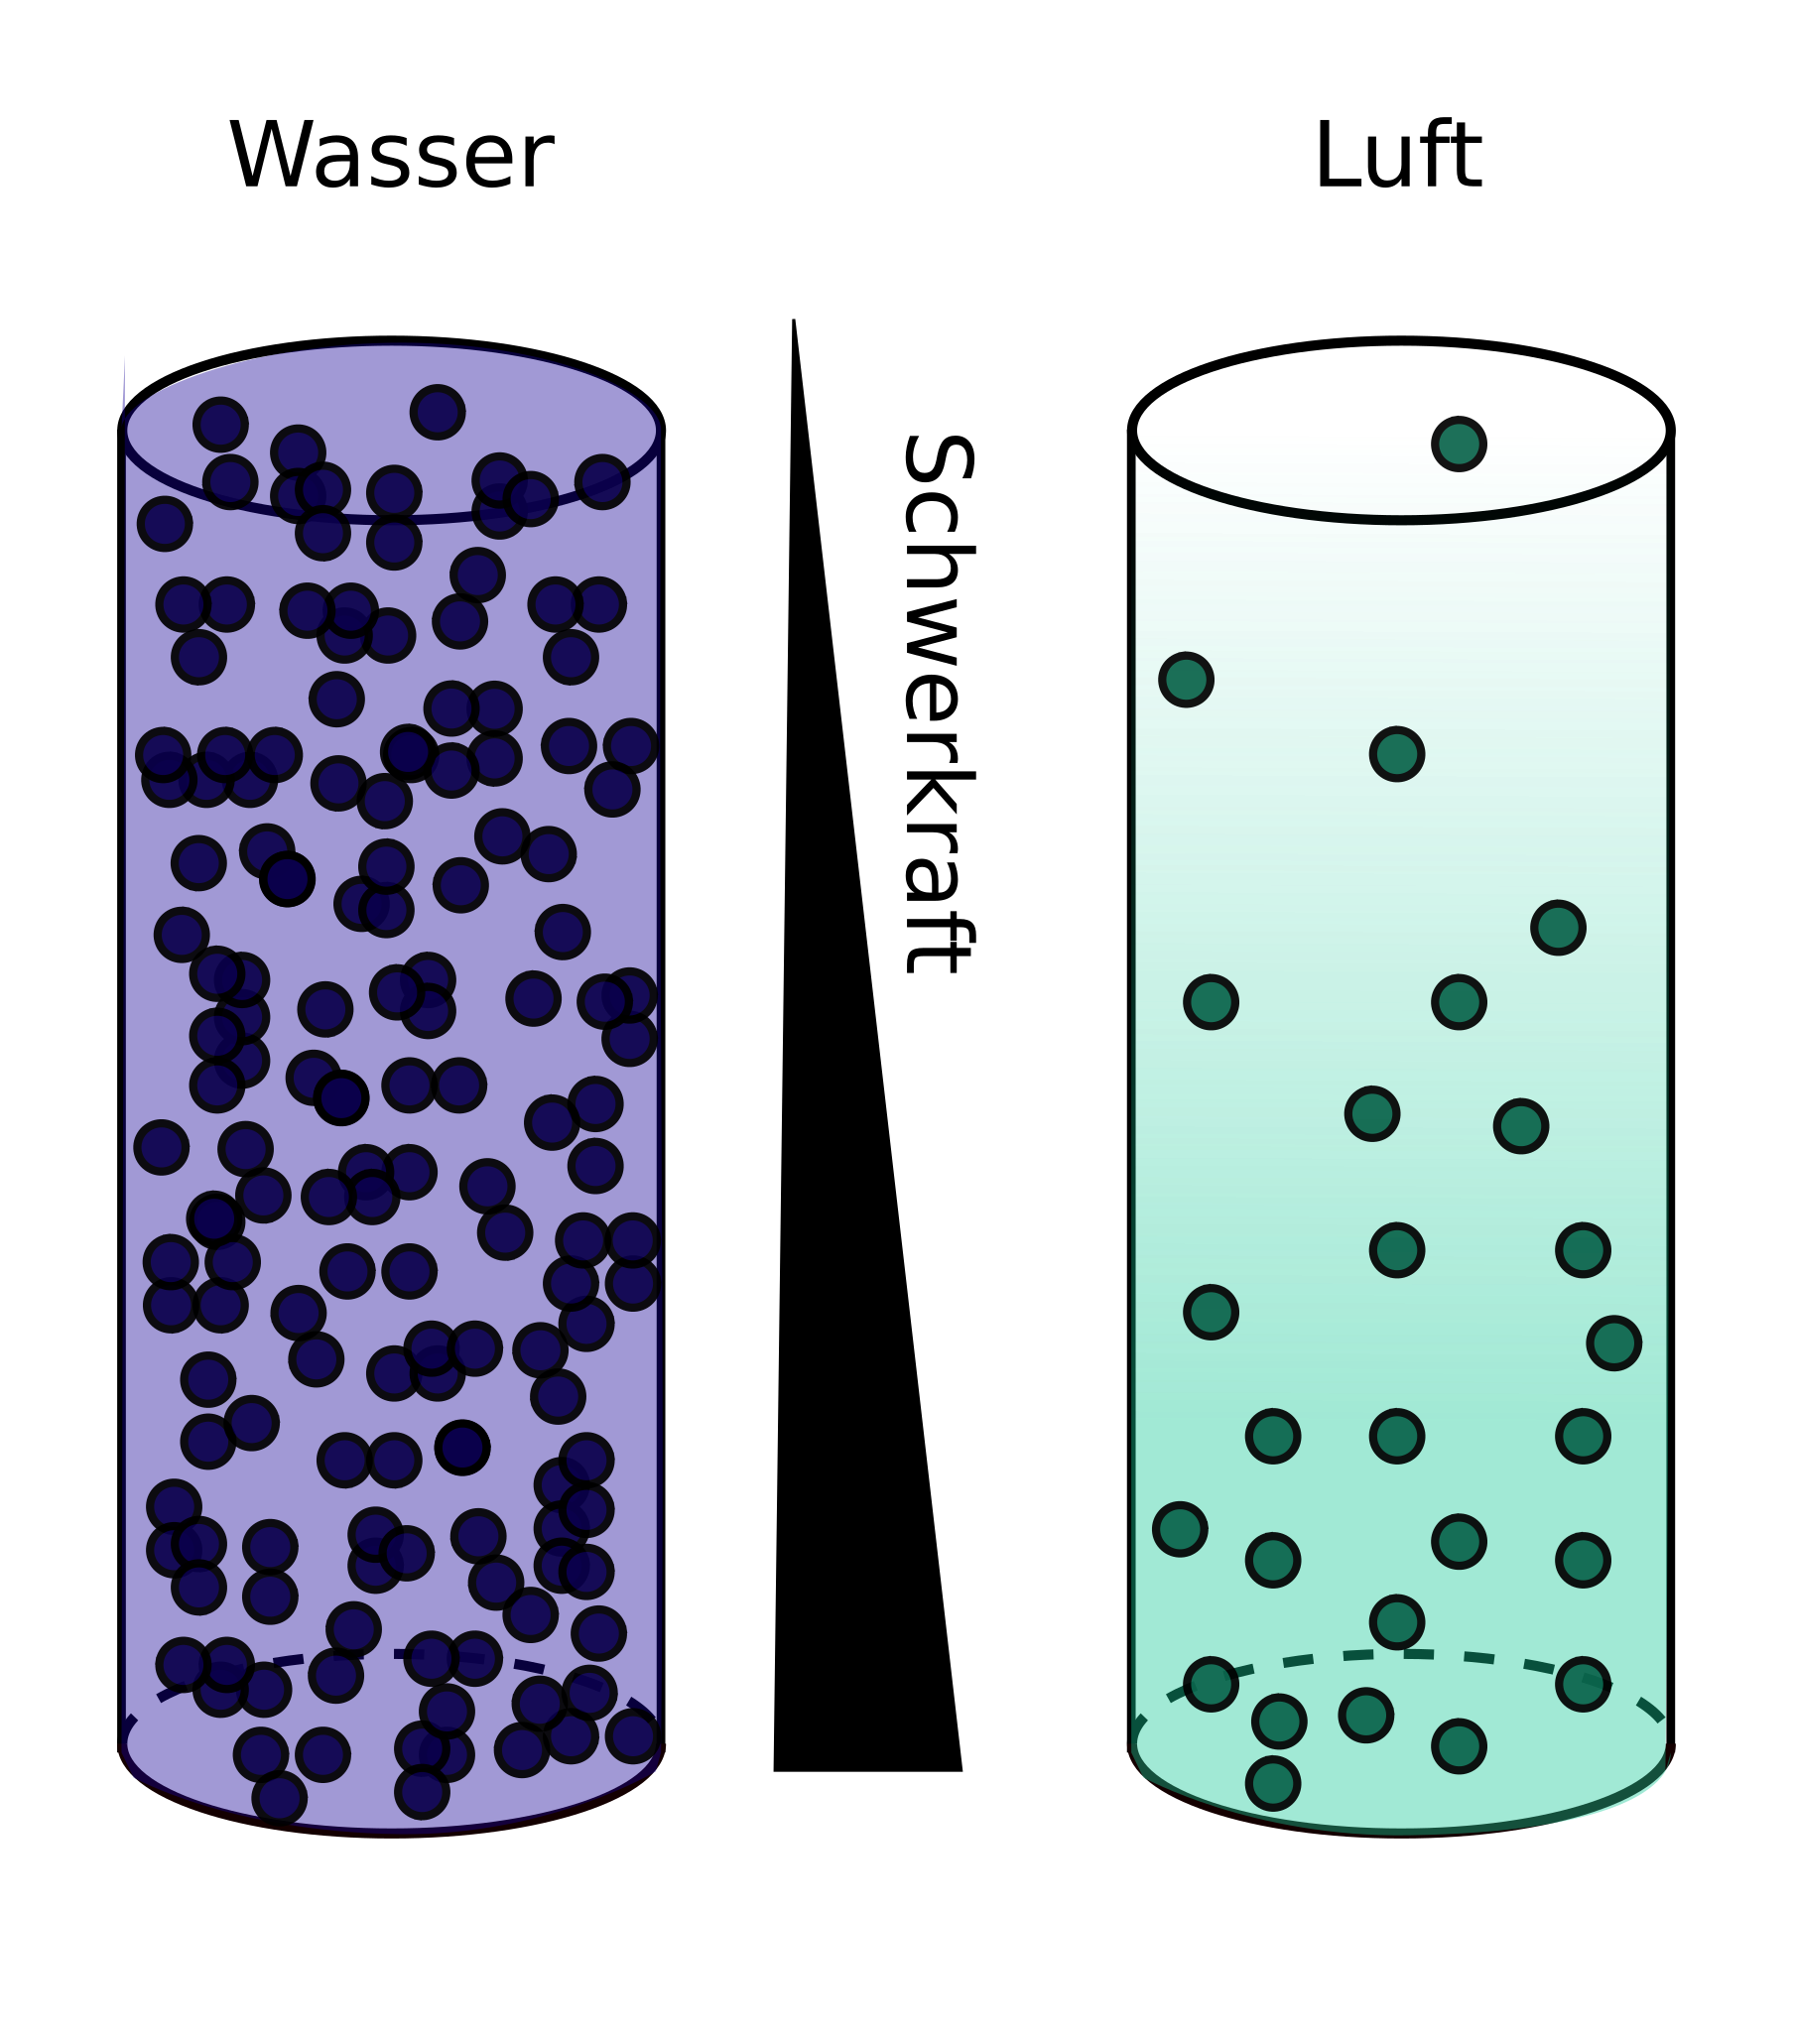
\includegraphics[width=\textwidth]{Wasserdruck_Luftdruck.png}
\end{center}
\end{column}
\end{columns}

\end{frame}



\begin{frame}
\frametitle{Luftdruck}

Faustregel: Abnahme um \(1\,\%\) alle \SI{80}{\meter} oder \(10\,\%\) alle \SI{840}{\meter} \\[0.5 cm]

\pause


Beispiel: 


\begin{tabular}{ll}
Atmosphärischer Druck am Meeresspiegel: & \(\sim\) \(10^5\,\frac{N}{m^2} = 1\,\text{bar}\) \\[0.2 cm]
Salzburg (\SI{424}{\meter}):            & \(\sim 0.99^5 \sim \, 0.95\, \text{bar}\) \\[0.2 cm]
Mauna Kea (\SI{4200}{\meter}):         & \(\sim 0.90^5 \sim \, 0.59\, \text{bar}\) \\[0.2 cm]
\end{tabular}


\end{frame}


%% Mauna Kea 
%% Übung: Symptome erklären?
\begin{frame}
\frametitle{Mauna Kea (\SI{4200}{\meter})}

\begin{columns}[c]

\begin{column}{5cm}

\begin{center}

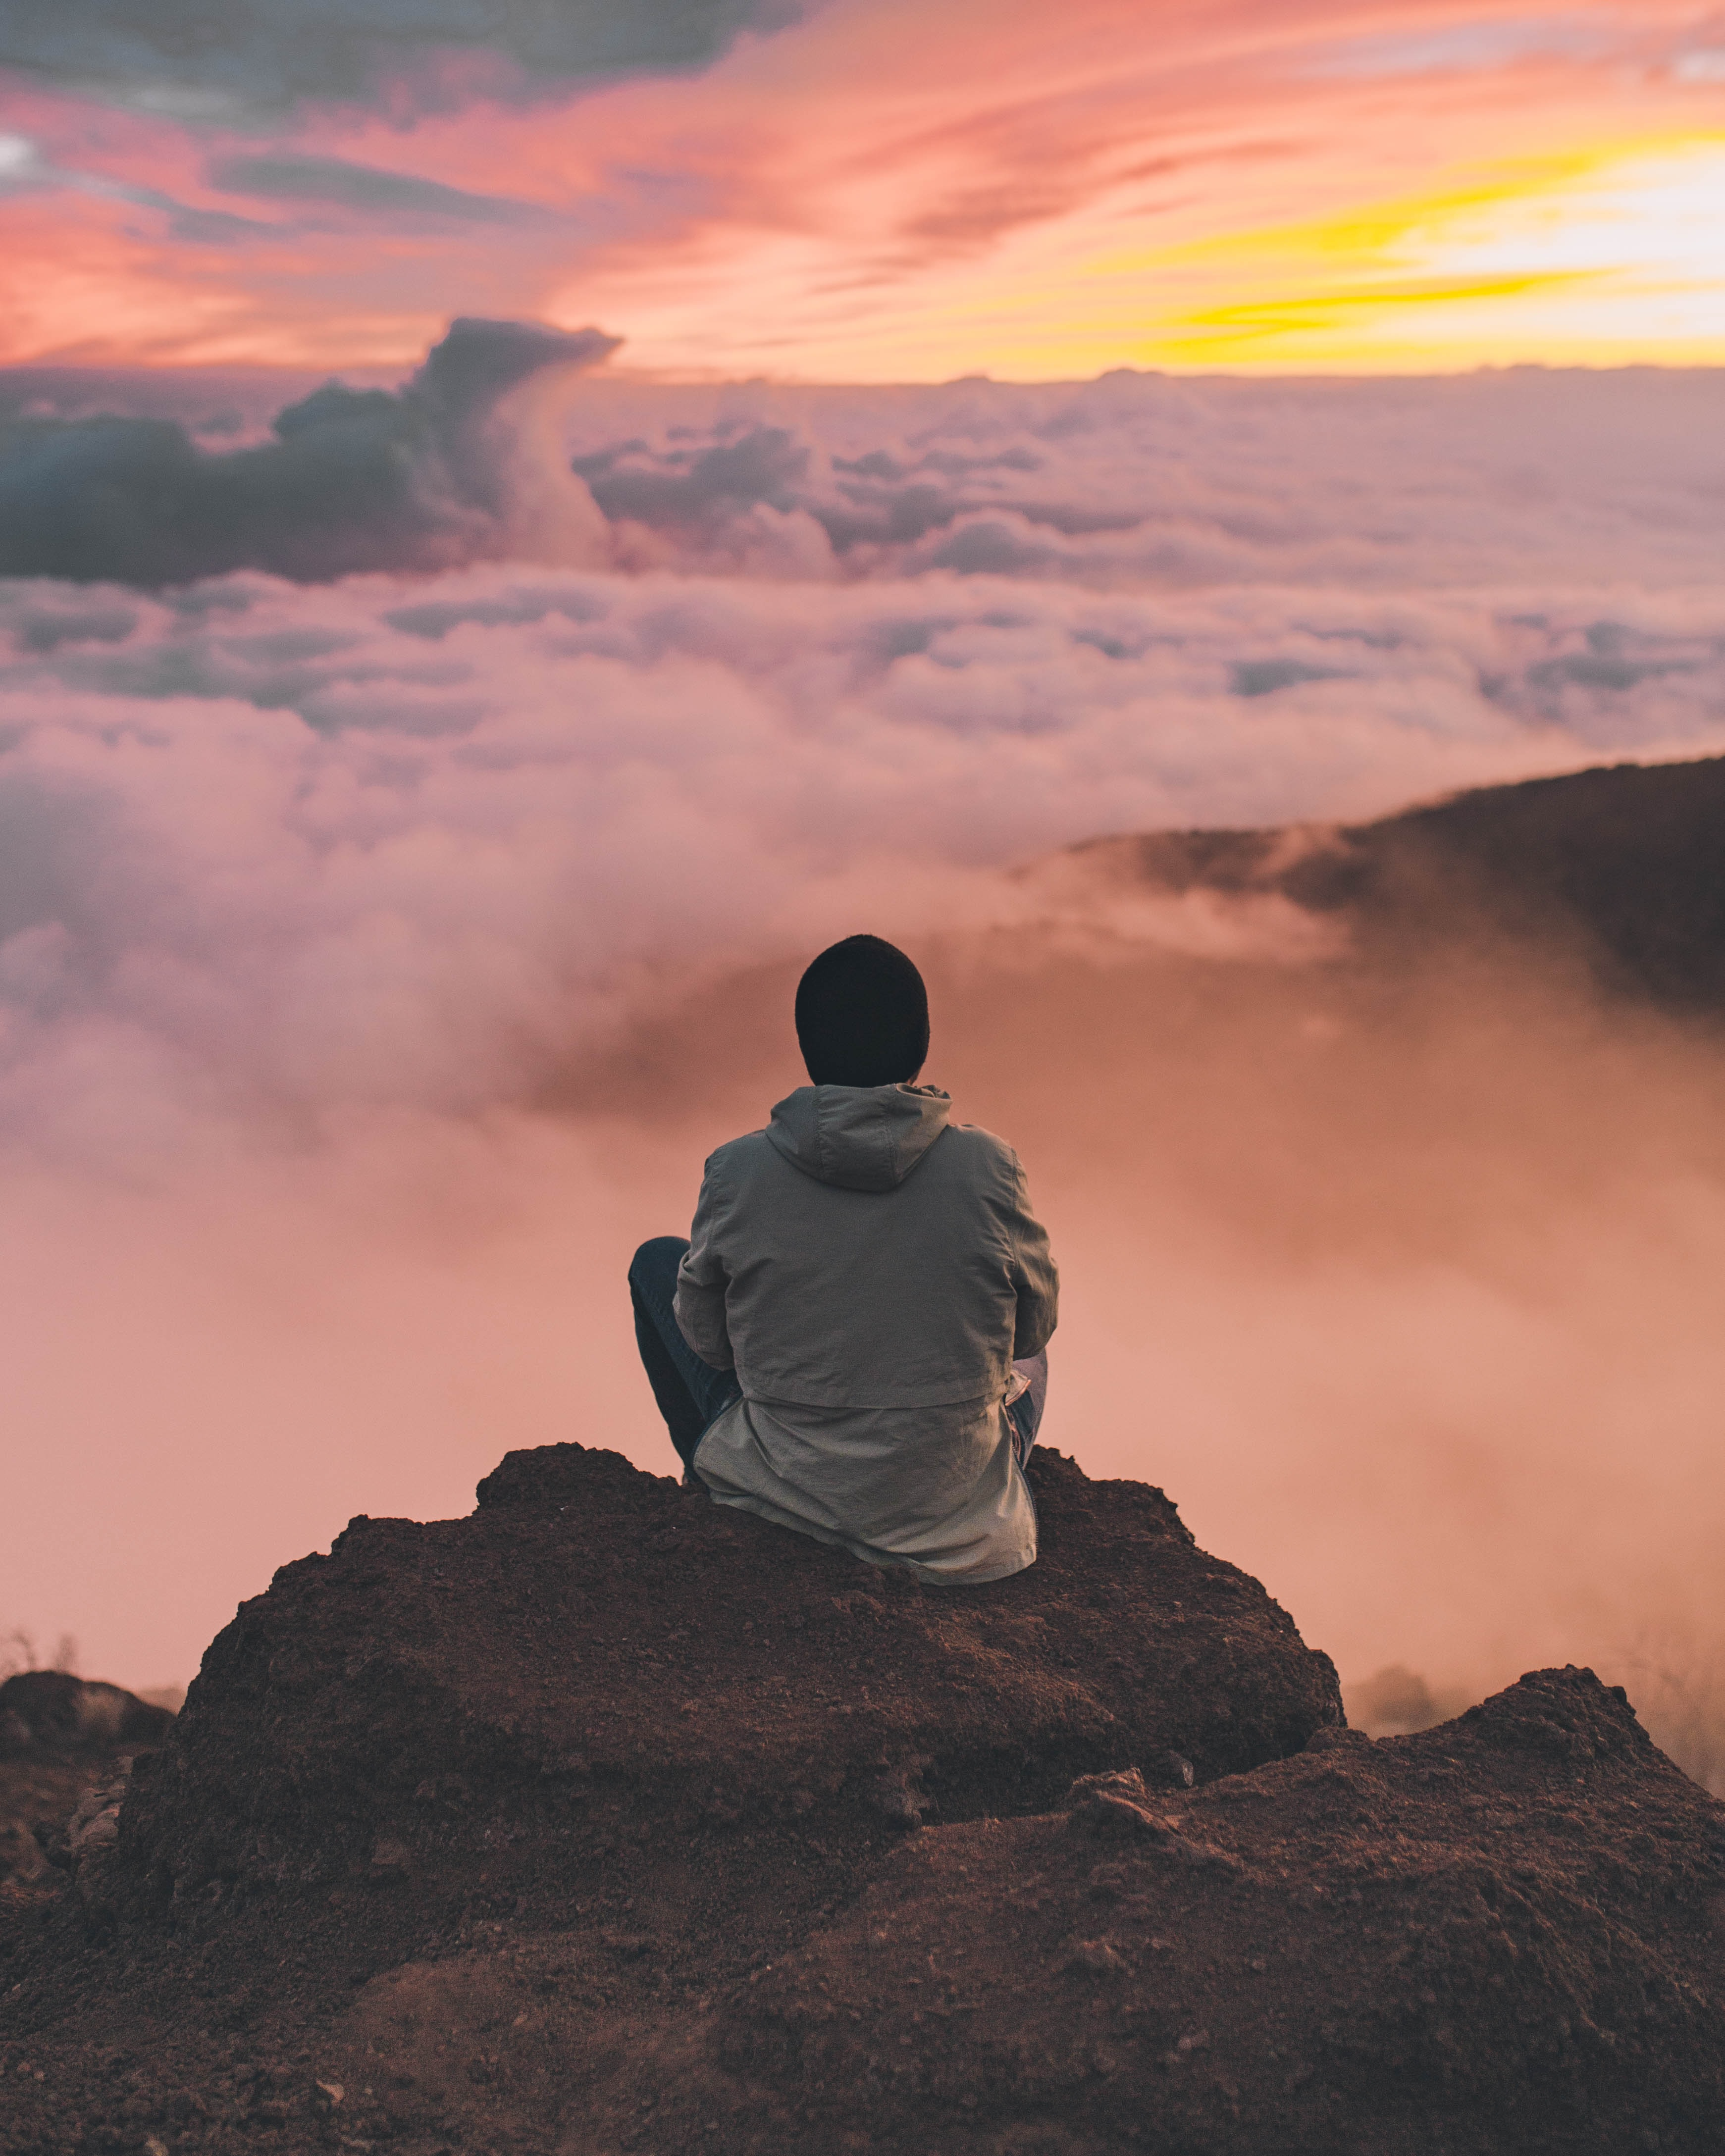
\includegraphics[width=\textwidth]{maunakea.jpg}

\end{center}

\end{column}

\begin{column}{5cm}

Leichte Kopfschmerzen, Atemnot, Übelkeit, Erschöpfung, Gedächtnisverlust, Konzentrationsschwierigkeiten, Appetitlosigkeit, Schlaflosigkeit \dots $\,$\\[0.5 cm]

Können wir einige dieser Symptome erklären?

\end{column}

\end{columns}

\end{frame}



%%%%%%%%%%%%%%%%%%%%
%%%%%%%%%%%%%%%%%%%%
%%%%%%%%%%%%%%%%%%%%



%% Definition und Einheit des Drucks,
%% Druckmessung,
%% Manometer,
%% atmosphärischer Luftdruck (Normdruck,
%% exponentielle Abnahme in Abhängigkeit von der
%% Höhe über dem Erdboden, Halbwertshöhe),



%% Druckerzeugung durch Stempel/Kolben (hy-
%% draulische Presse),
%% Druck in elastisch gedehnten Gefäßen,
%% Beziehung zwischen Druck und mechanischer
%% Spannung bei Hohlorganen (s.a. GK Physiol.
%% 3.4.1, 4.1.1 und 5.4.1



%% Schweredruck in Flüssigkeiten,
%% Abhängigkeit von der Eintauchtiefe,
%% Entstehung des Auftriebs,
%% archimedisches Prinzip

%% Taucherkrankheit,
%% Wassergymnastik


%% Druckerzeugung durch Stempel/Kolben (hy-
%% draulische Presse),
%% Druck in elastisch gedehnten Gefäßen,
%% Beziehung zwischen Druck und mechanischer
%% Spannung bei Hohlorganen (s.a. GK Physiol.
%% 3.4.1, 4.1.1 und 5.4.1)

%% Nucleus pulposus,
%% Infusomat,
%% Blutdruckmessung nach Riva-Rocci,
%% Mechanik des Herzens,
%% Alveole





\section{Strömung}

%%%%%%%%%%%%%%%%
%% LO: 
%%%%%%%%%%%%%%%%

%% \item
%%  Strömungswiderstand, Strömungsleitwert definieren 
%% \item

%% \item
%%  Strömungswiderstand, Strömungsleitwert berechnen
%% Die Kirchhoff-Gesetze anwenden



%%%%%%%%%%%%%%%%%%%%


%% Volumenstrom definieren
\begin{frame}
\frametitle{Volumenstrom}


\begin{center}
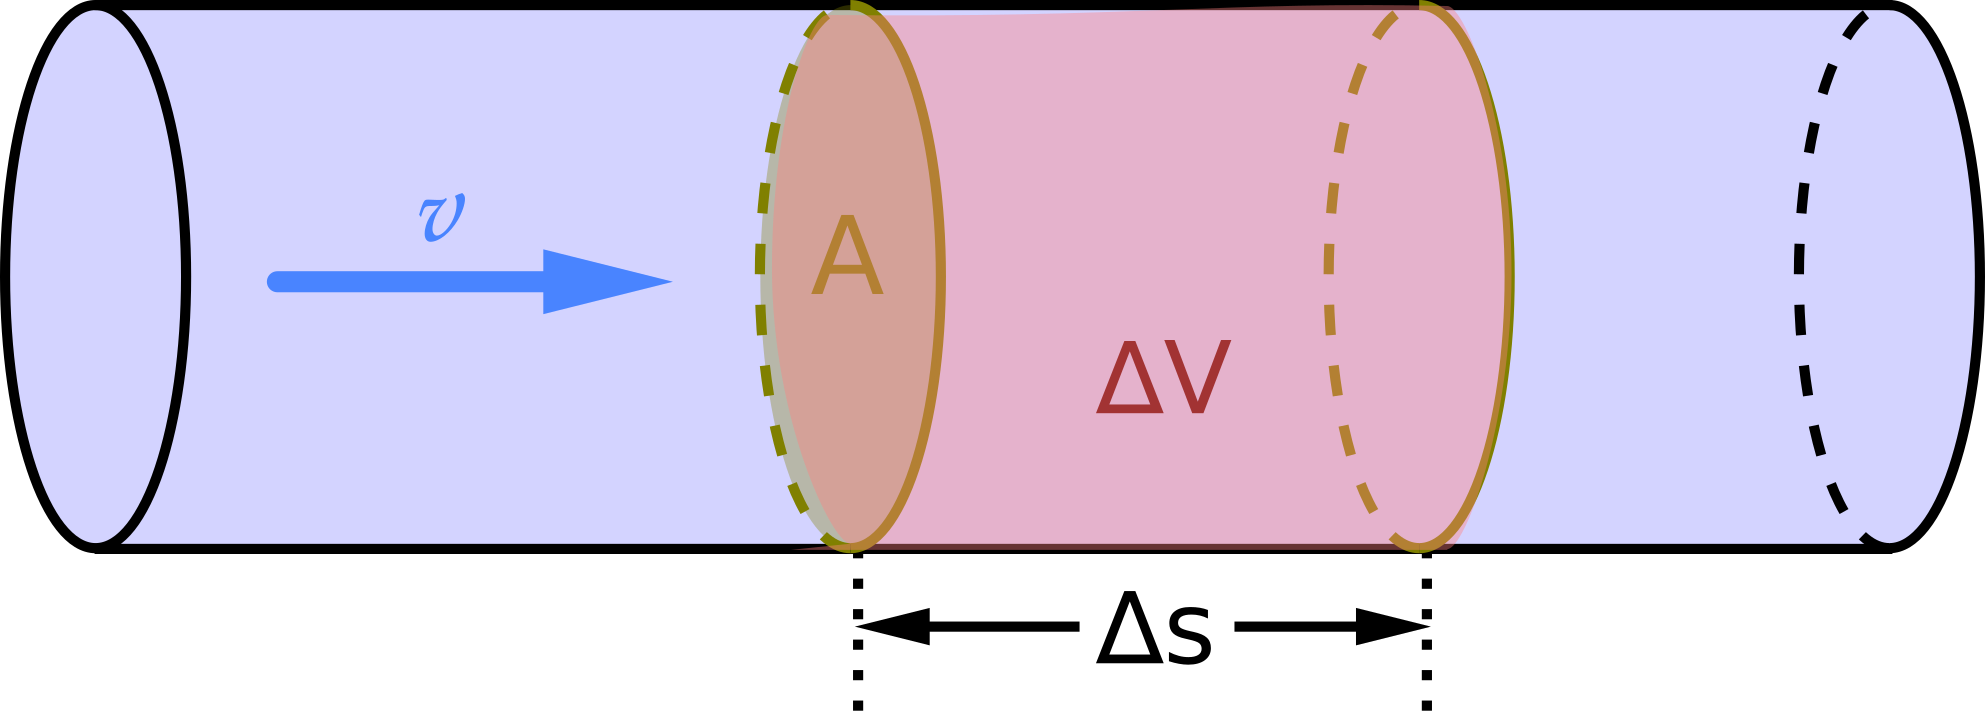
\includegraphics[width=\textwidth]{volumenstrom.png}
\end{center}

Volumenstromstärke:
 
\[
I = \frac{\Delta V}{\Delta t} = \mathcalligra{v}\times A  \qquad \text{Einheit: } \frac{m^3}{s}
\]

\end{frame}


\begin{frame}
\frametitle{Volumenstrom: Beispiel}

\begin{columns}[c]
\begin{column}{5cm}

\begin{center}
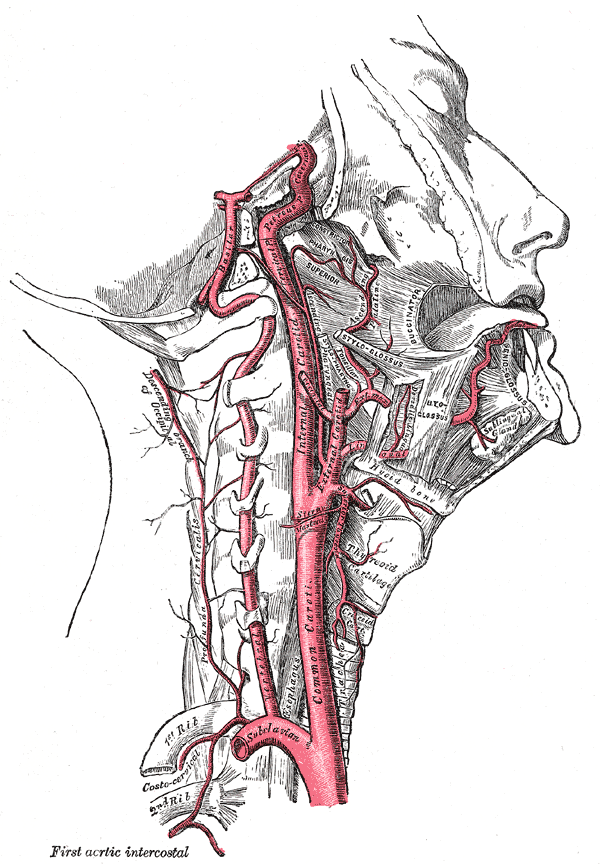
\includegraphics[width=\textwidth]{halsarterien.png}
\end{center}


\end{column}

\begin{column}{5cm}

Innere Halsschlagader: \SI{200}{\milli\liter\per\minute}. Wieviel ist das in \SI{}{\cubic\meter\per\second}?

\pause

\[
200 \frac{\text{ml}}{\text{min}} \times 10^{-6} \frac{\text{m}^3}{\text{ml}} \times \frac{1}{60} \frac{\text{min}}{\text{s}} \approx
\]

\[
\approx 3\times 10^{-6} \frac{\text{m}^3}{\text{s}}
\]

\end{column}



\end{columns}

\end{frame}


%% Kontinuitätsgleichung kennen und anwenden

\begin{frame}
\makebox[\linewidth]{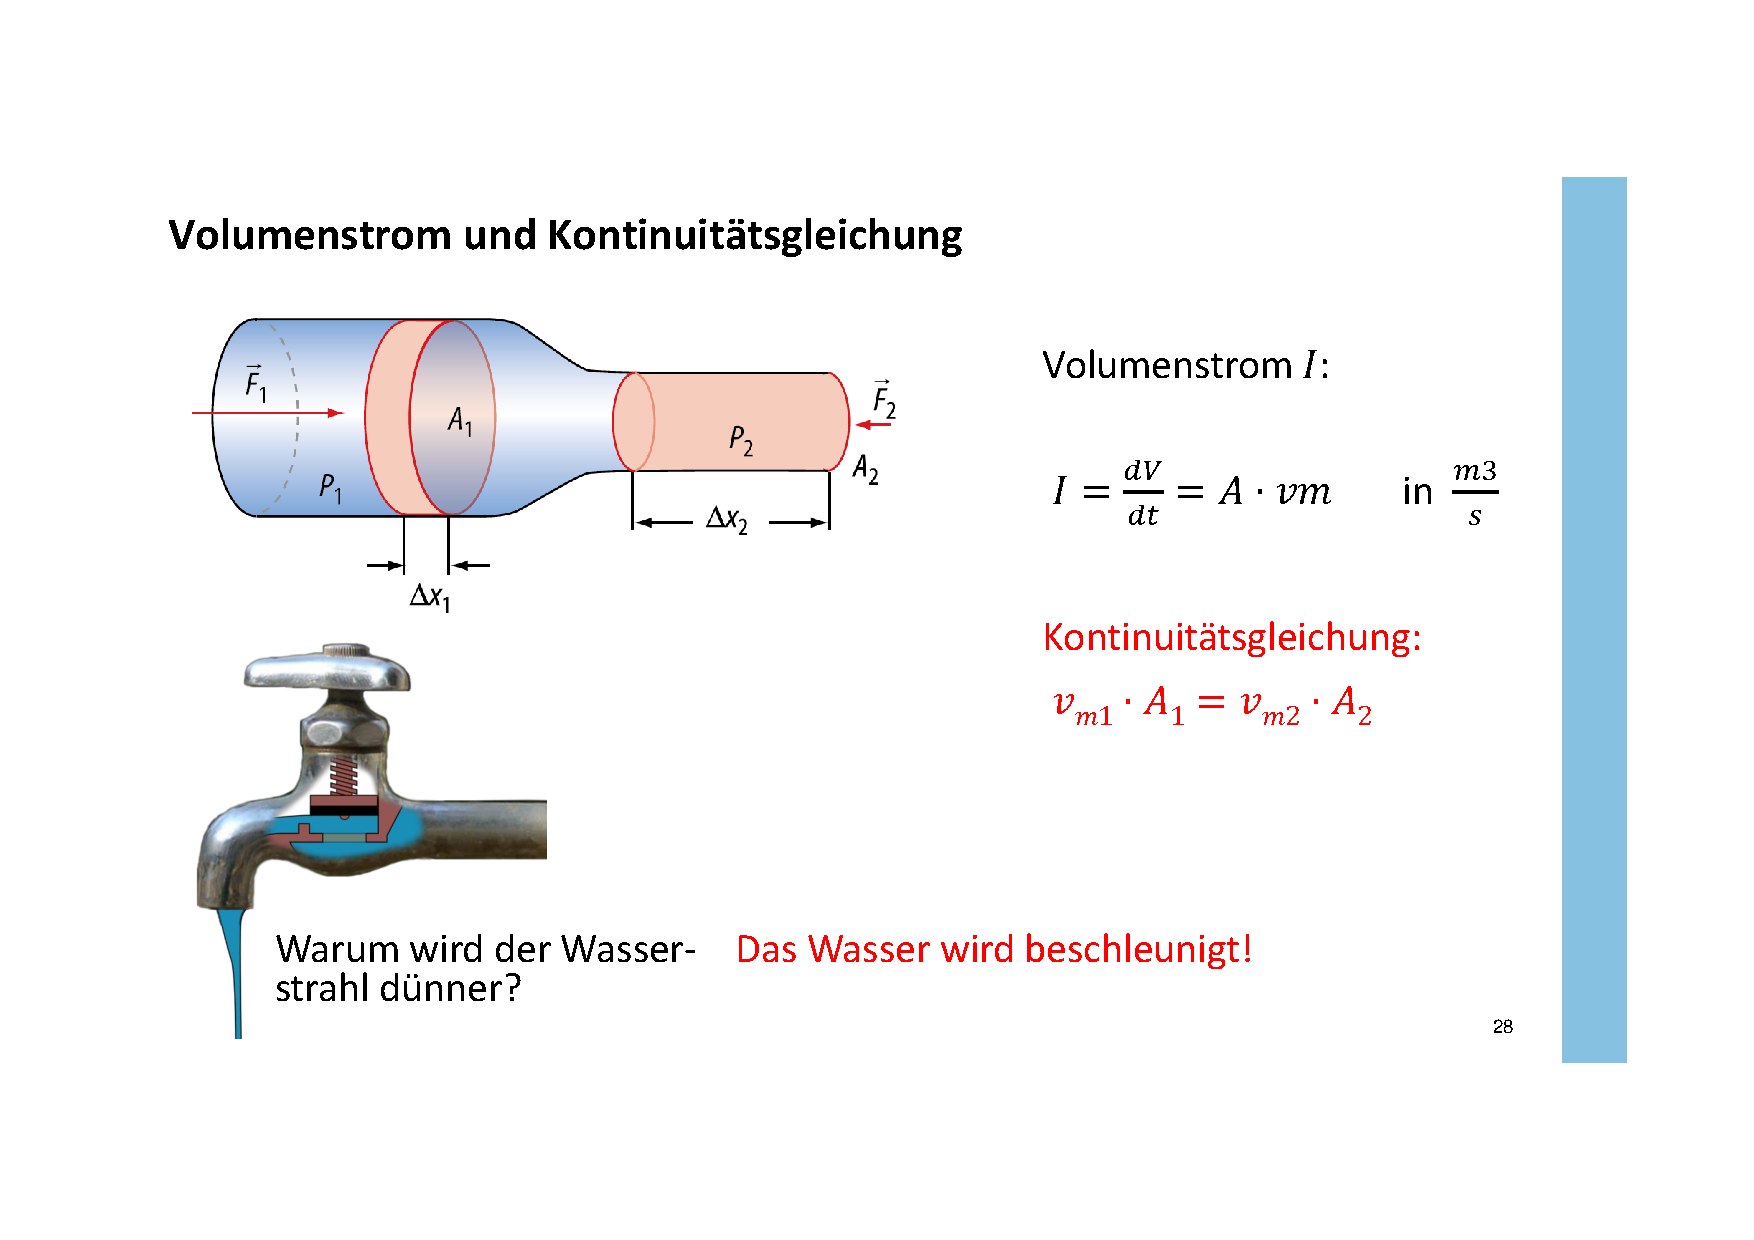
\includegraphics[width=\textwidth]{Walter_Druck_Kontinuitaetsgleichung.pdf}}
\end{frame}


\begin{frame}
\frametitle{Kontinuitätsgleichung: Beispiel}
\begin{center}
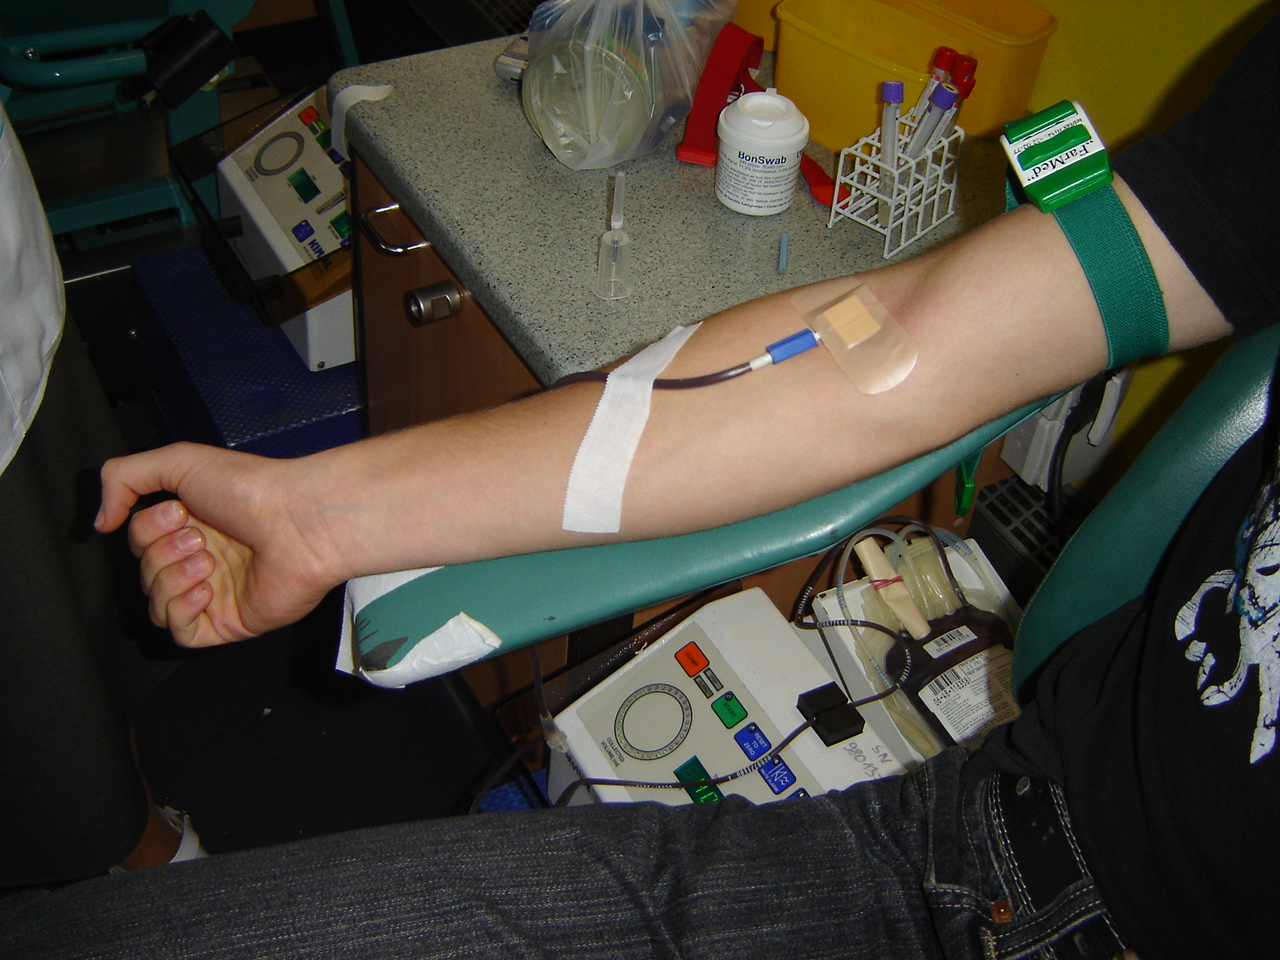
\includegraphics[width=\textwidth]{blutspende.JPG}
\end{center}
\end{frame}

%% Darstellungen eines Strömungsfeldes durch Stromlinien verstehen und erstellen

\begin{frame}
\makebox[\linewidth]{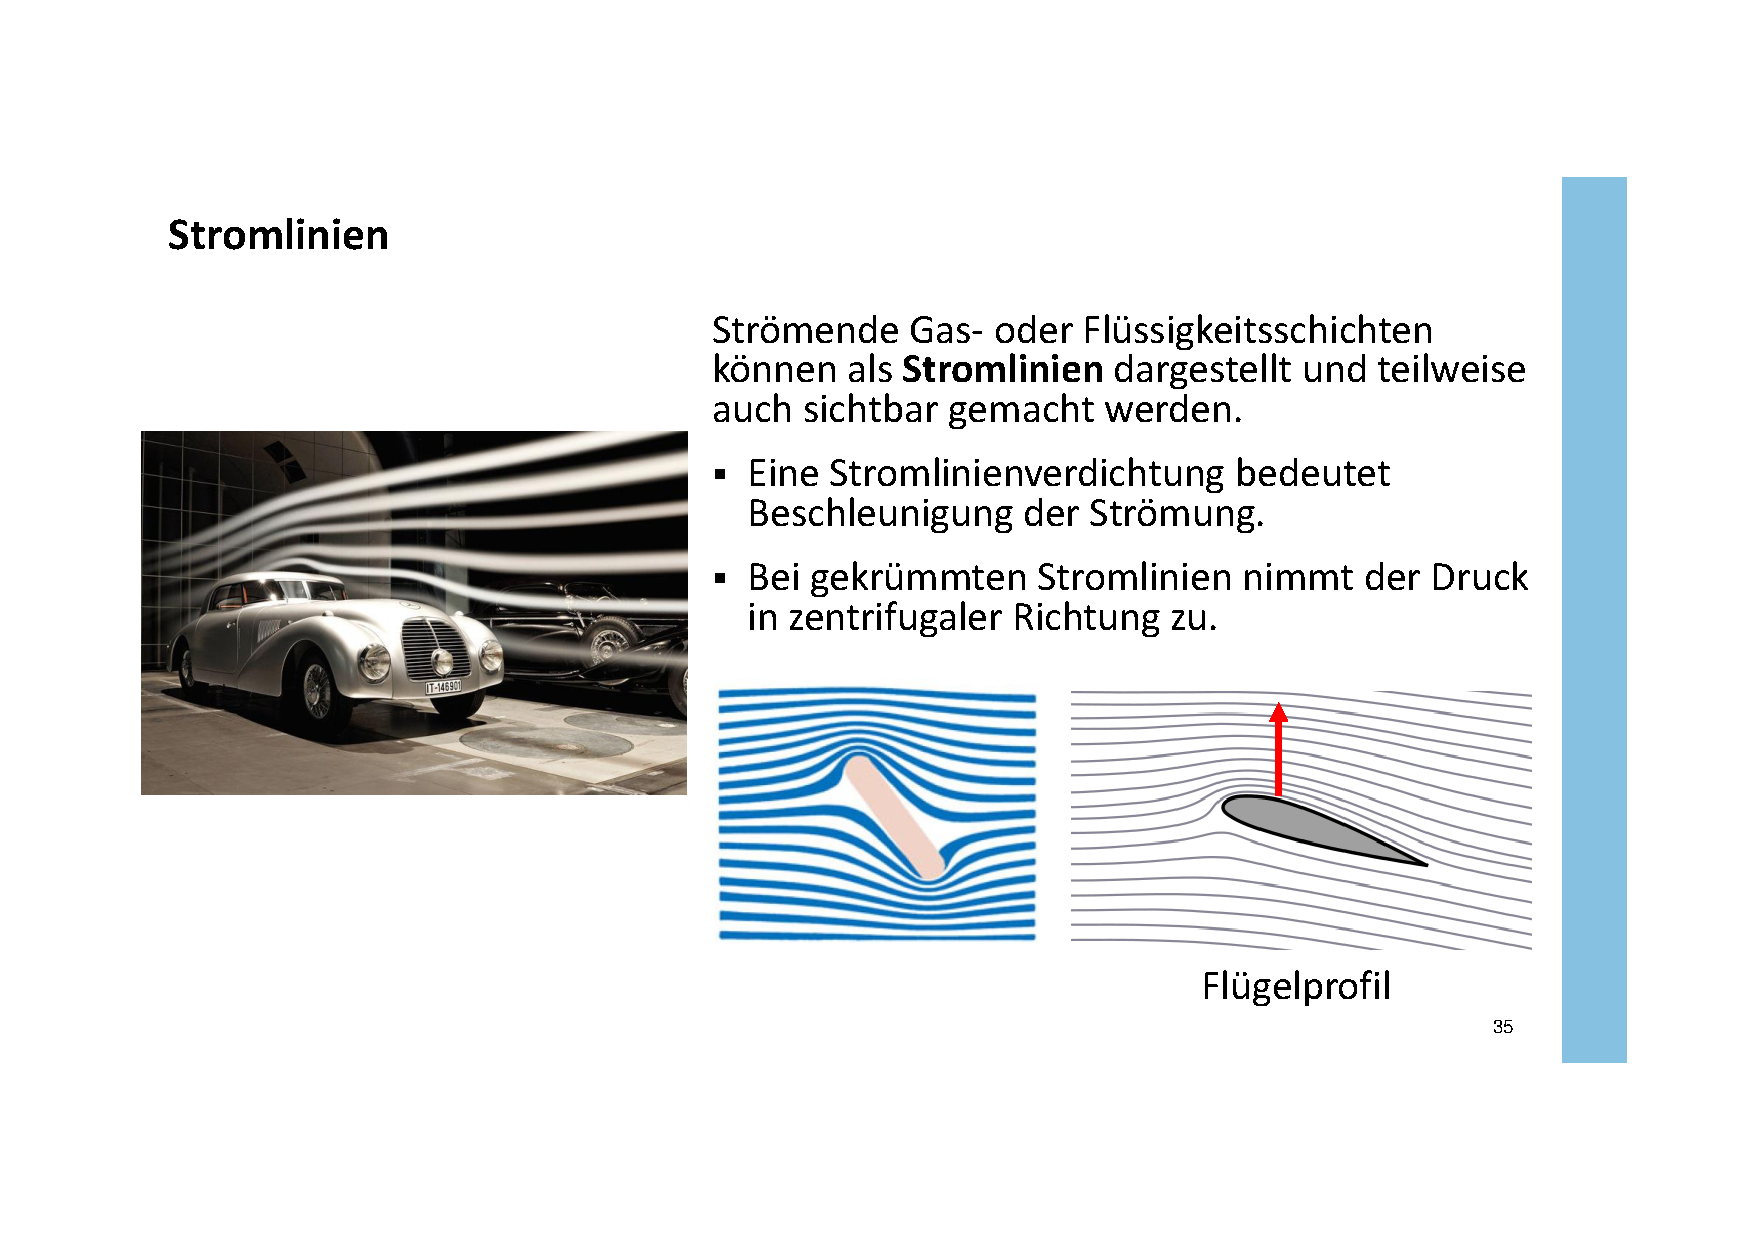
\includegraphics[width=\textwidth]{Walter_Druck_Stromlinien.pdf}}
\end{frame}



%% Bernoulli-Effekt, Hydrodynamisches Paradoxon

\begin{frame}
\frametitle{Gesetz von Bernoulli}

Der Gesamtdruck ist auf einer Stromlinie konstant. \\[0.5 cm]

\pause

Gesamtdruck = Statischer Druck + dynamischer Druck + Schweredruck \\[0.5 cm]


\begin{tabular}{ll}
Gesamtdruck     & \(p_{\text{ges}}\)     \\[0.2 cm]
Statischer Druck        & \(p_0\)  (senkrecht zur Strömung)   \\[0.2 cm]
Dynamischer Druck       & (auch: ``Staudruck'') \pause - ? \\
\end{tabular}


\end{frame}

\begin{frame}
\frametitle{Gesetz von Bernoulli - Dynamischer Druck}

\begin{center}
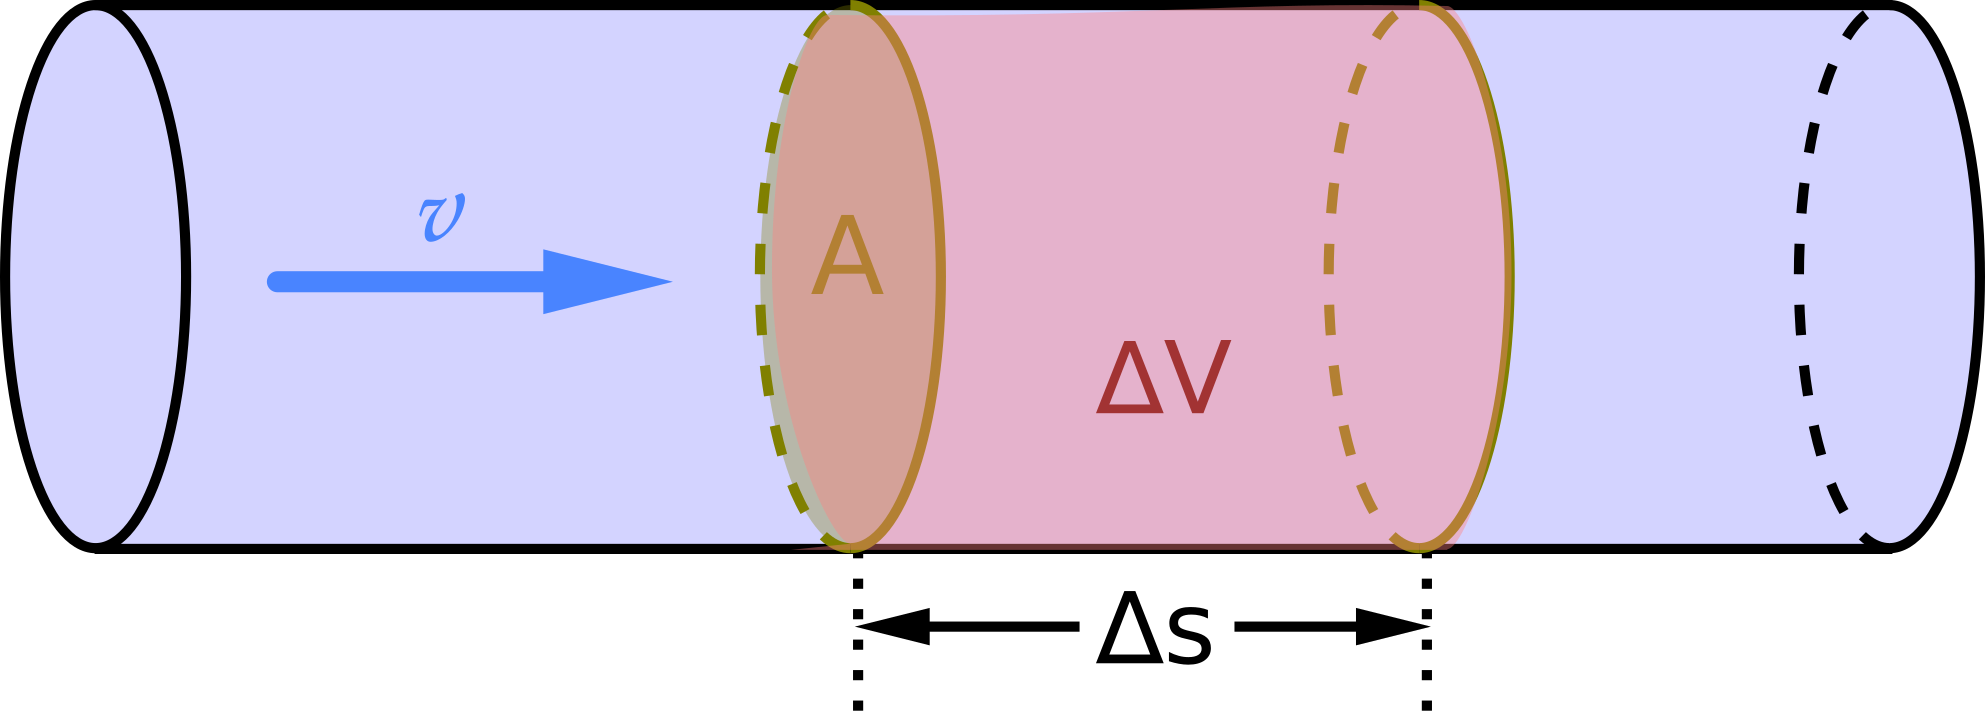
\includegraphics[width=0.5\textwidth]{volumenstrom.png}
\end{center}

Kinetische Energie:

\[
E_{\text{kin}} = \frac{1}{2} m v^2
\]

\pause
Masse: 

\[
m = \rho * V
\]

\pause
Dynamischer Druck: Kinetische Energie pro Volumen

\[
p_{\text{dyn}} = \frac{E_{\text{kin}}}{V} =  \frac{1}{2} \rho v^2
\]


\end{frame}


\begin{frame}
\frametitle{Gesetz von Bernoulli}



Gesamtdruck = Statischer Druck + dynamischer Druck + Schweredruck \\[0.5 cm]


\begin{tabular}{ll}
Gesamtdruck     & \(p_{\text{ges}}\)     \\[0.2 cm]
Statischer Druck        & \(p_0\)     \\[0.2 cm]
Dynamischer Druck       & \(\frac{1}{2}\rho v^2\) \\[0.2 cm]
Schweredruck    & ? \\
\end{tabular}


\end{frame}


\begin{frame}
\frametitle{Gesetz von Bernoulli}

Gesamtdruck = Statischer Druck + dynamischer Druck + Schweredruck \\[0.5 cm]


\begin{tabular}{ll}
Gesamtdruck     & \(p_{\text{ges}}\)     \\[0.2 cm]
Statischer Druck        & \(p_0\)     \\[0.2 cm]
Dynamischer Druck       & \(\frac{1}{2}\rho v^2\) \\[0.2 cm]
Schweredruck    & dürfen wir vernachlässigen \\[0.5 cm]
\end{tabular}

\pause

\[
p_{\text{ges}} = p_0 + \frac{1}{2}\rho v^2 = \text{konstant auf einer Stromlinie}
\]


\end{frame}

%% Papier blasen
\begin{frame}
\frametitle{Kleines Experiment}

\pause

Warum? 

\end{frame}



\begin{frame}
\frametitle{Kleines Experiment}

\[
p_{\text{ges}} = p_0 + \frac{1}{2}\rho v^2 = \text{konstant auf einer Stromlinie}
\]

\(\rightarrow\) Wenn sich die Strömungsgeschwindigkeit erhöht, muss sich \(p_0\) verkleinern.
\end{frame}


\begin{frame}
\frametitle{Verständnisfrage}

\begin{columns}[c]
\begin{column}{5cm}
\begin{center}
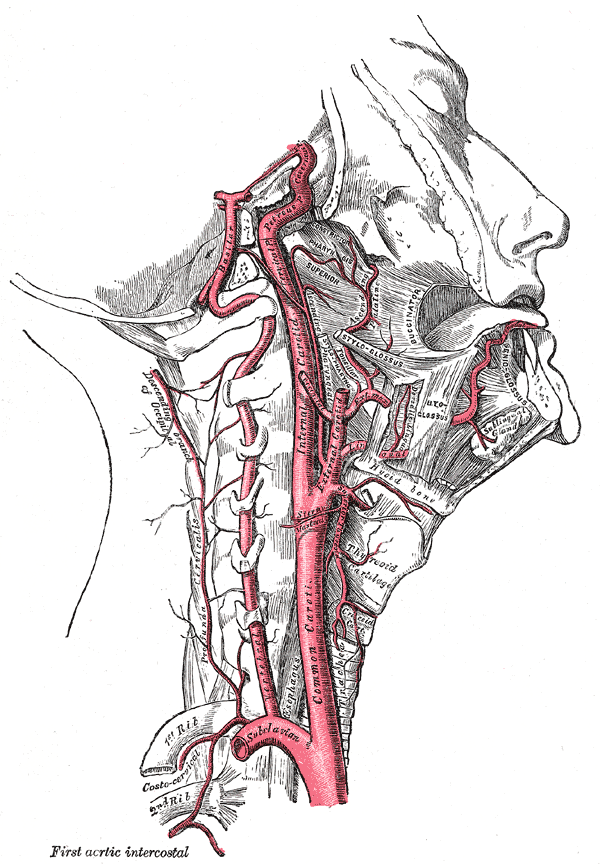
\includegraphics[width=\textwidth]{halsarterien.png}
\end{center}
\end{column}

\begin{column}{5cm}

\begin{itemize}
\item
Wie schnell flie{\ss}t Blut in kleinen vs gro{\ss}en Blutgefä{\ss}en?
\item
Wie verhält es sich mit dem Blutdruck?
\end{itemize}

\pause

In \textcolor{theme}{kleineren} Blutgefäßen fließt das Blut \textcolor{theme}{schneller}, und der Druck ist \textcolor{theme}{geringer}. 


\end{column}
\end{columns}


\end{frame}


%% Viskosität
\begin{frame}
\frametitle{Stimmt das immer genau?}

\pause
\begin{columns}[c]
\begin{column}{5cm}

Nein, auch bei Flüssigkeiten und Gasen gibt es (ähnlich wie bei festen Körpern) Reibungsverluste. \\

Innere Reibung (Viskosität) hängt davon ab, wie stark Teilchen innerhalb einer Flüssigkeit aneinander binden. 

\end{column}

\begin{column}{5cm}
\begin{center}
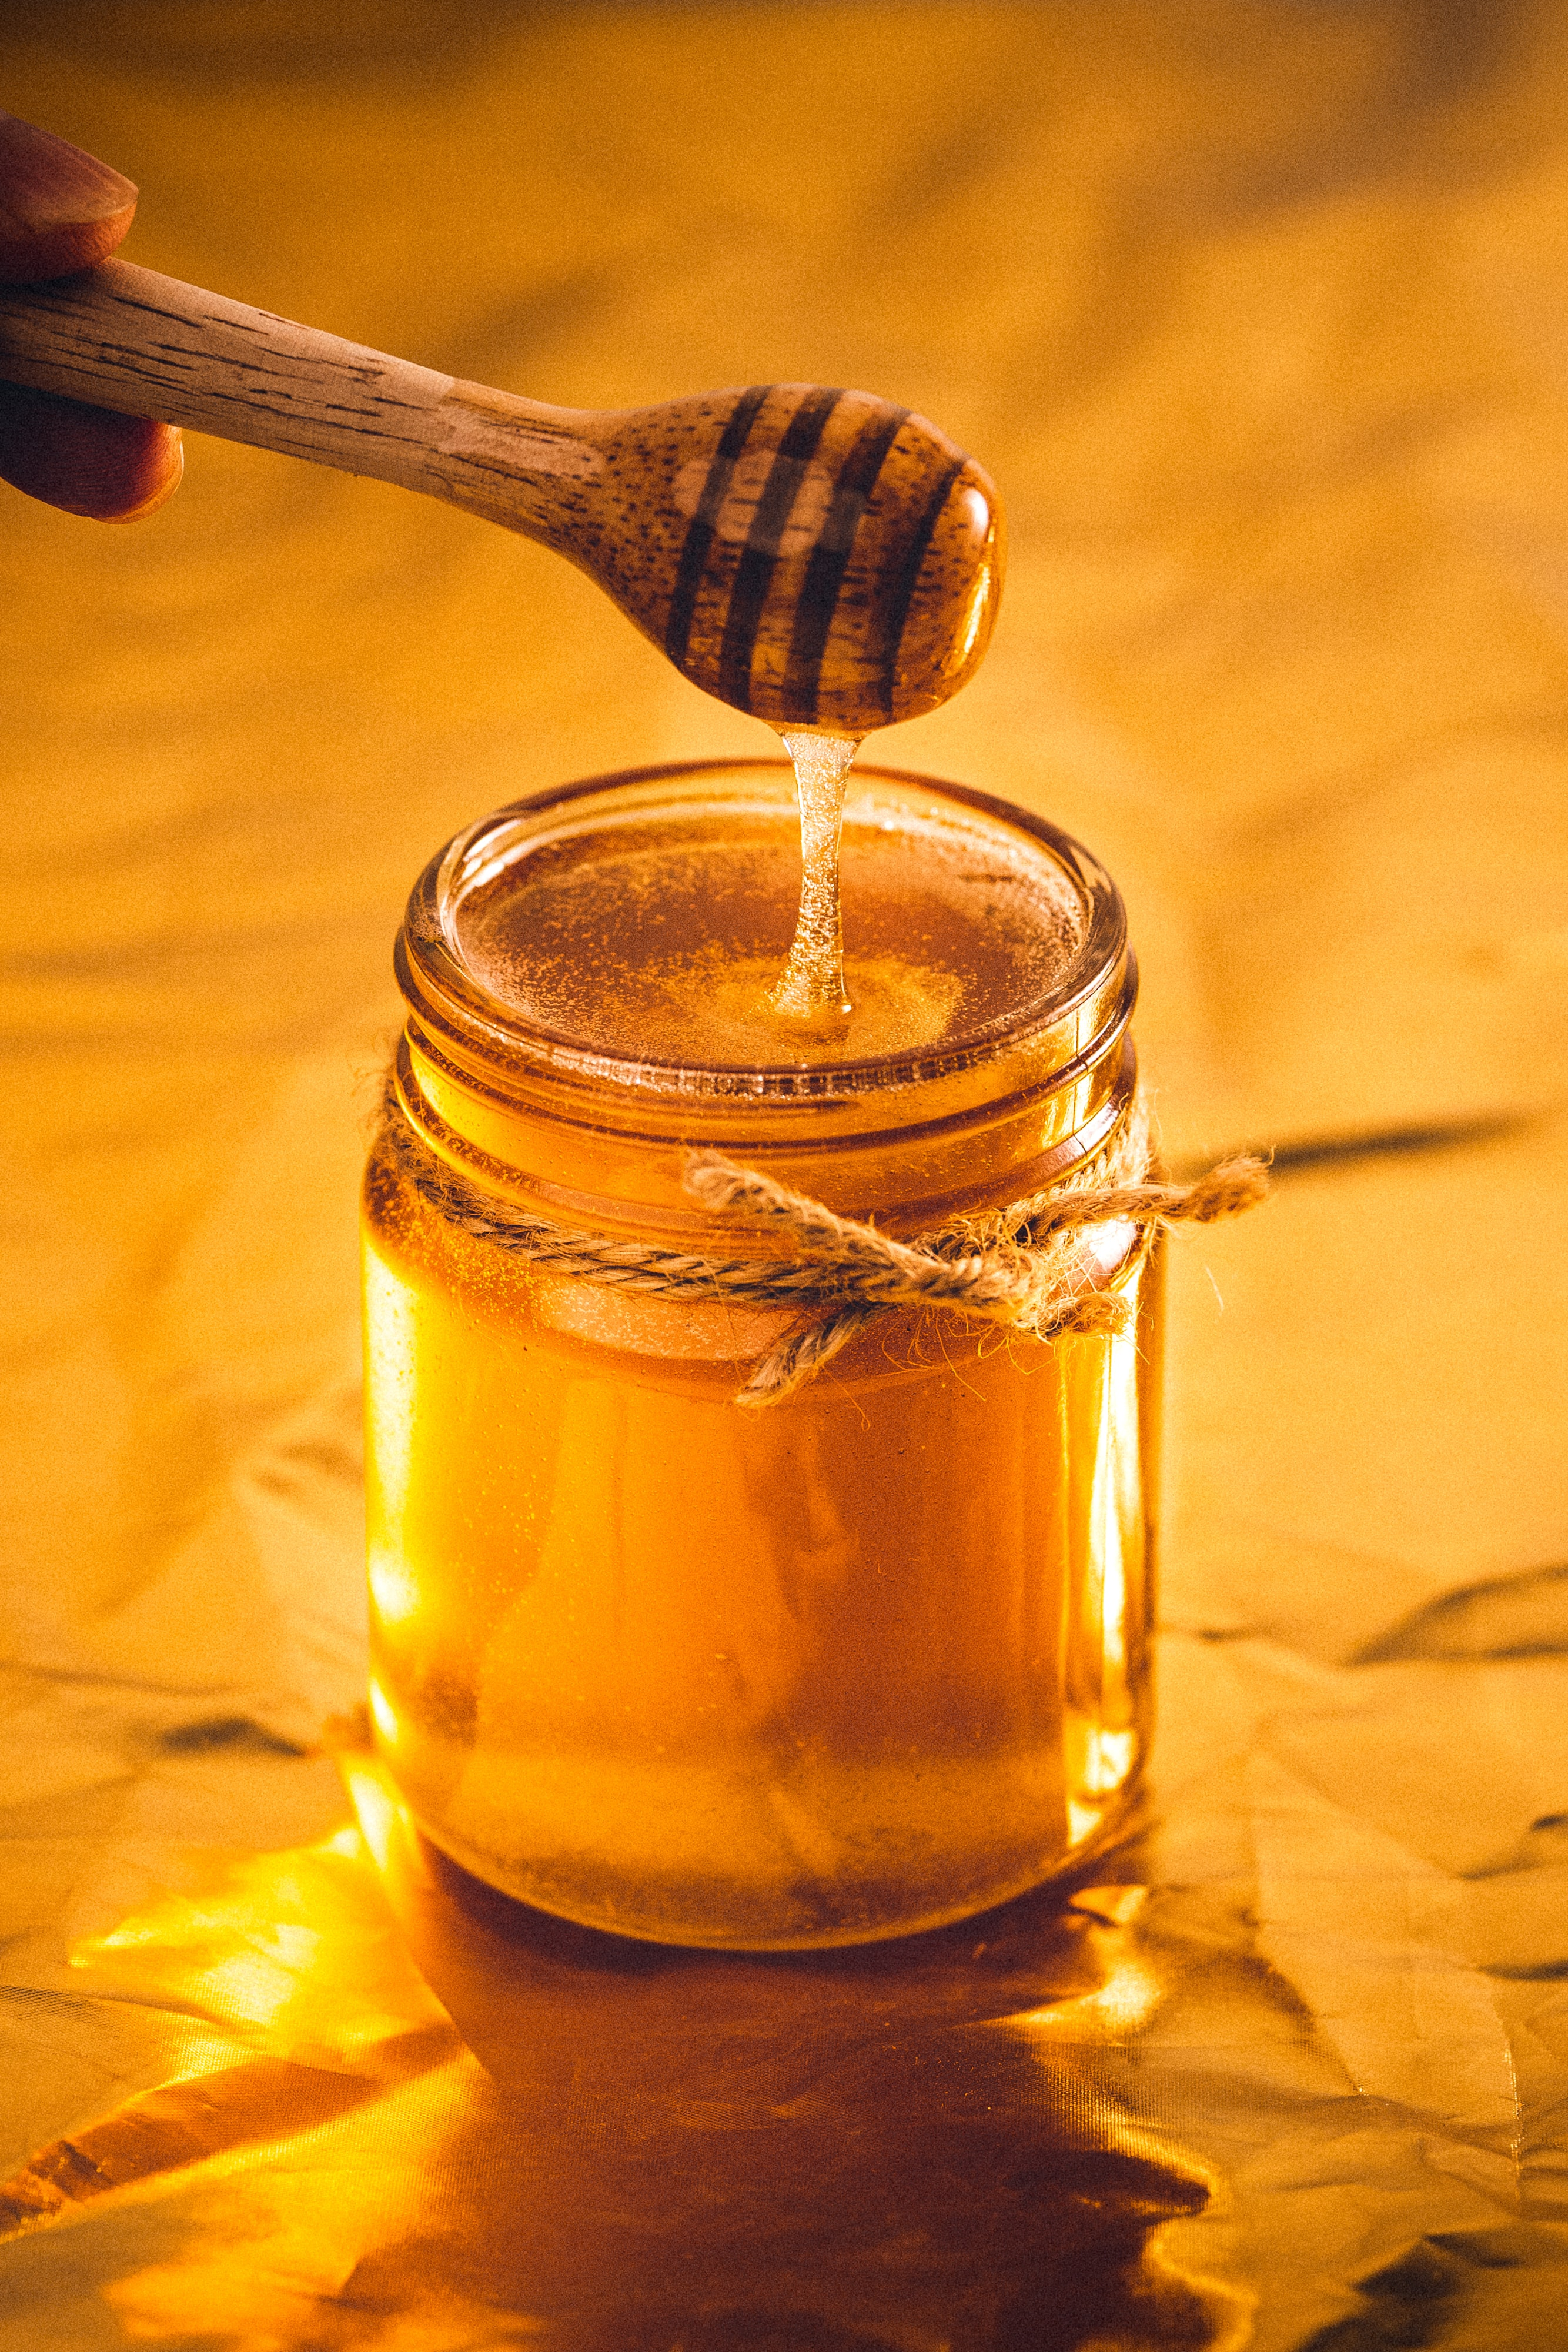
\includegraphics[width=\textwidth]{honey.jpg}
\end{center}
\end{column}

\end{columns}

\end{frame}


%% Das Hagen-Poiseuille Gesetz anwenden

\begin{frame}
\makebox[\linewidth]{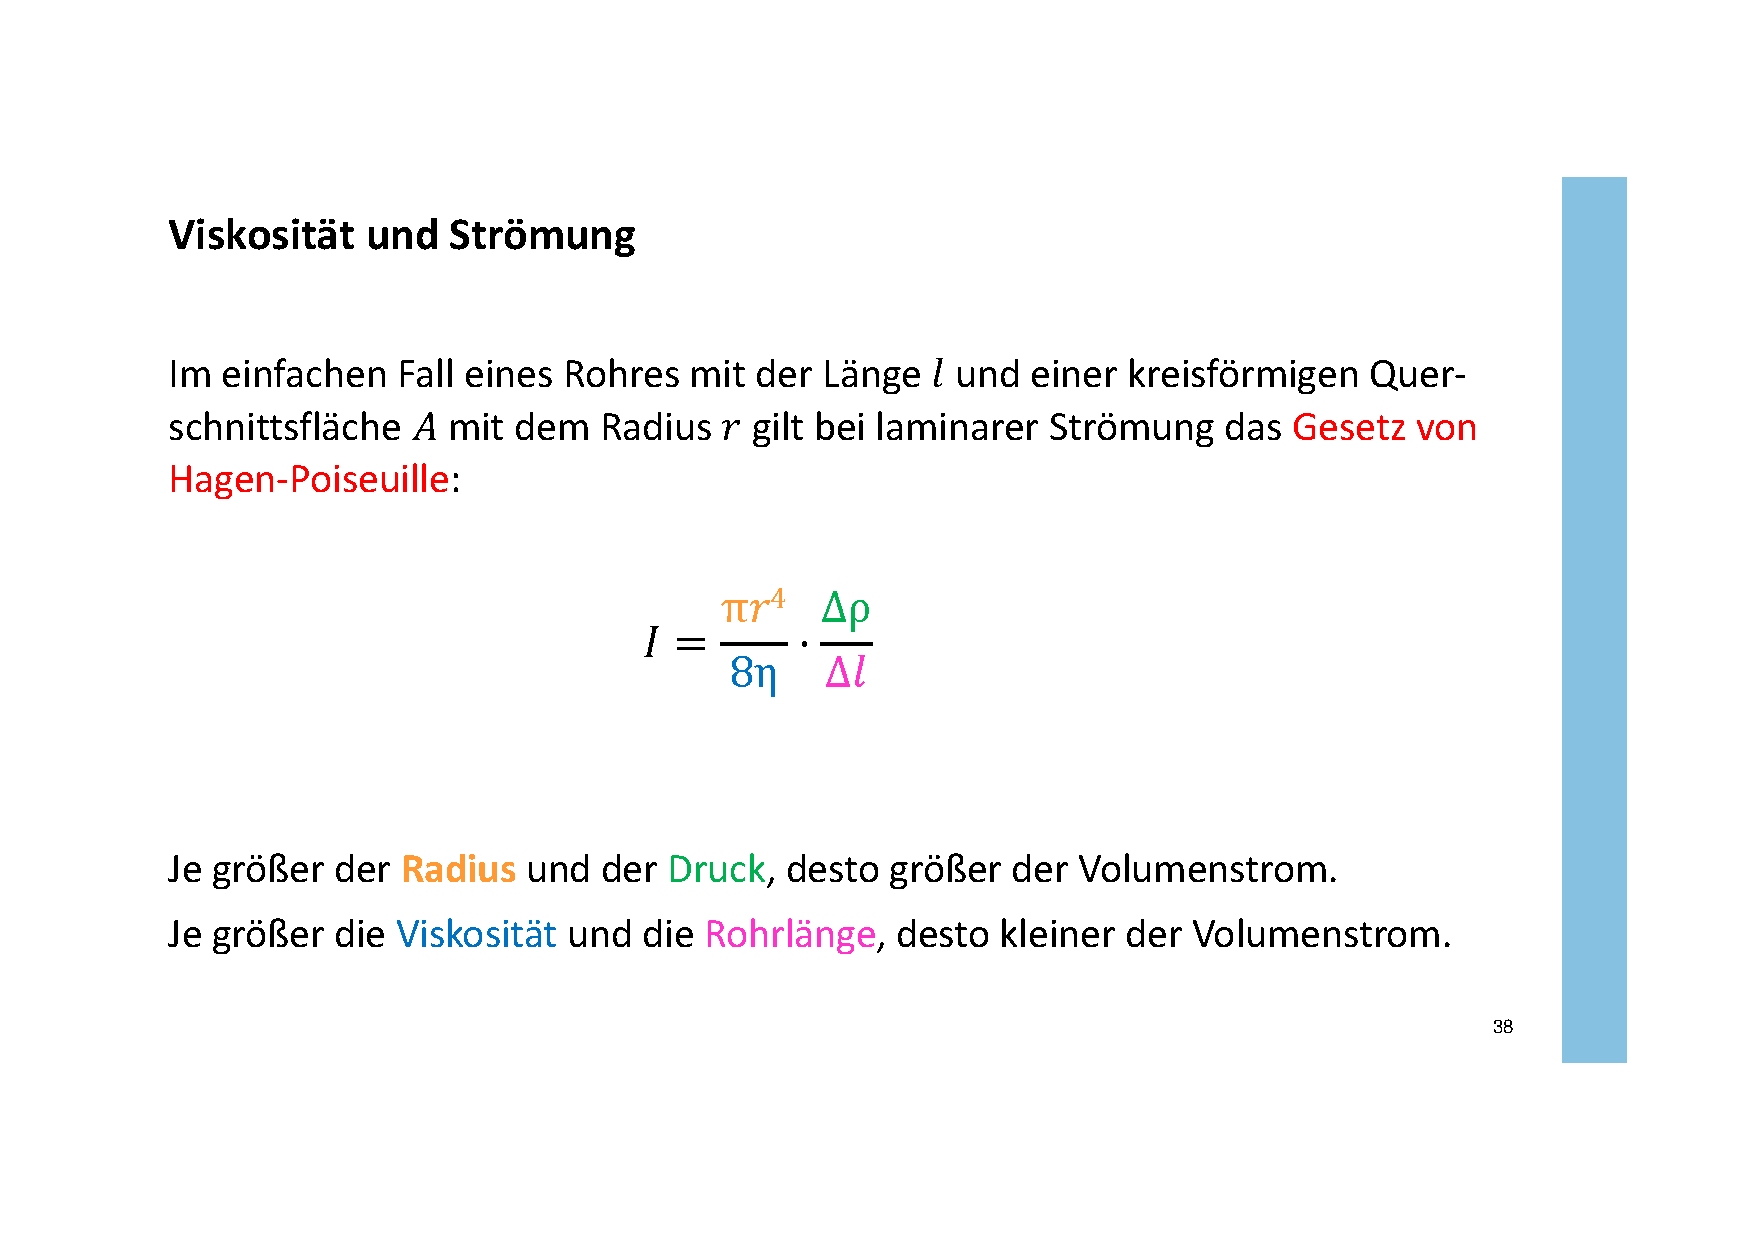
\includegraphics[width=\textwidth]{Walter_Druck_Hagen_Poiseuille.pdf}}
\end{frame}


%% Strömungswiderstand
\begin{frame}
\frametitle{Strömungswiderstand}

Strömungswiderstand: 

\[
R = \frac{8 \eta \Delta l}{\pi r^4}
\]

\pause

Damit lässt sich das Gesetz von Hagen-Poiseuille auch schreiben als

\[
I = \frac{\Delta p}{R}
\]

\pause

Strömungsleitwert \(G = \frac{1}{R}\)


\end{frame}


\begin{frame}
\frametitle{Strömungswiderstand}

\begin{columns}[c]

\begin{column}{5cm}

\[
I = \frac{\Delta p}{R}
\]

Kommt uns das bekannt vor?


\pause

\begin{center}
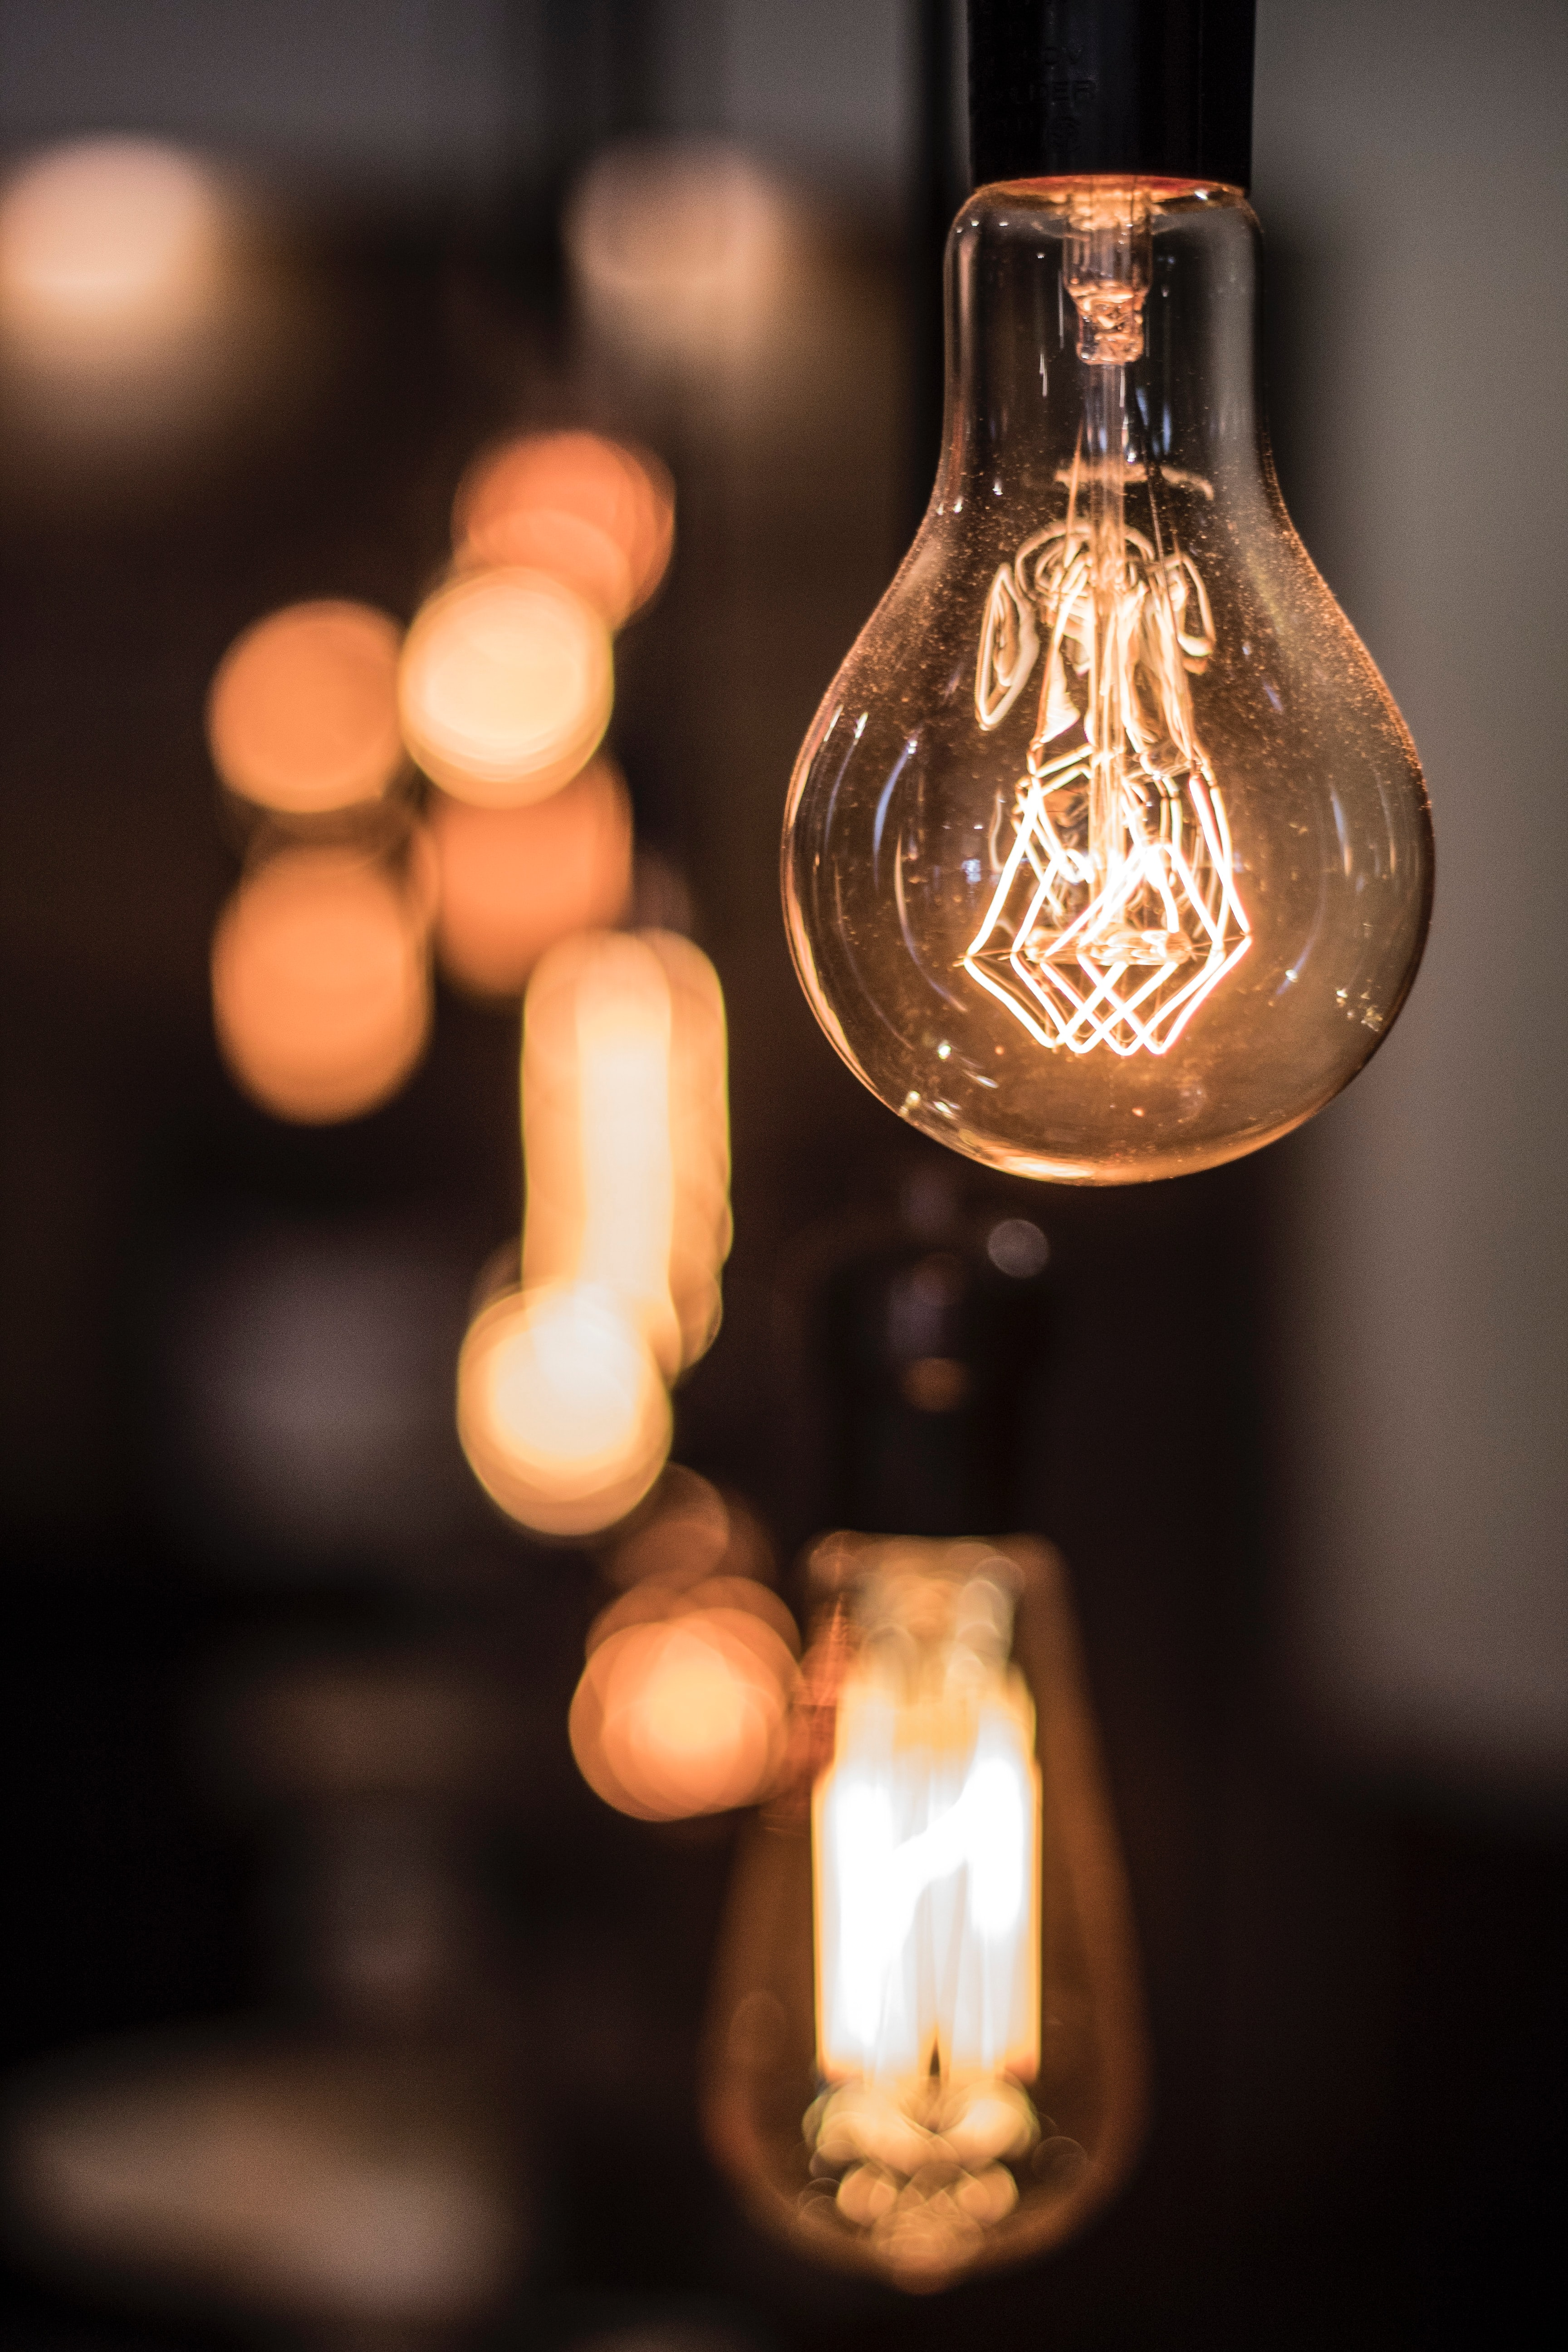
\includegraphics[width=0.6\textwidth]{lightbulb.jpg}
\end{center}



\end{column}

\begin{column}{5cm}



Stromstärke = Spannung durch Widerstand

\[
I = \frac{A}{R}
\]

\end{column}

\end{columns}

\end{frame}

\begin{frame}
\frametitle{Flüssigkeitsstrom verhält sich wie elektrischer Strom!}

\begin{columns}[c]

\begin{column}{7cm}
Insbesondere gilt (Kirchhoff-Gesetze):
\begin{itemize}
\item
Bei Reihenschaltungen addieren sich die Widerstände zum Gesamtwiderstand 
\[
R_{\text{gesamt}} = \sum_{n=1}^N R_n
\]

\item
Bei Parallelschaltungen addieren sich die Kehrwerte der Widerstände zum Kehrwert des Gesamtwiderstands 
\[
\frac{1}{R_{\text{gesamt}}} = \sum_{n=1}^N \frac{1}{R_n}
\]


\end{itemize}
\end{column}

\begin{column}{4cm}

\begin{center}
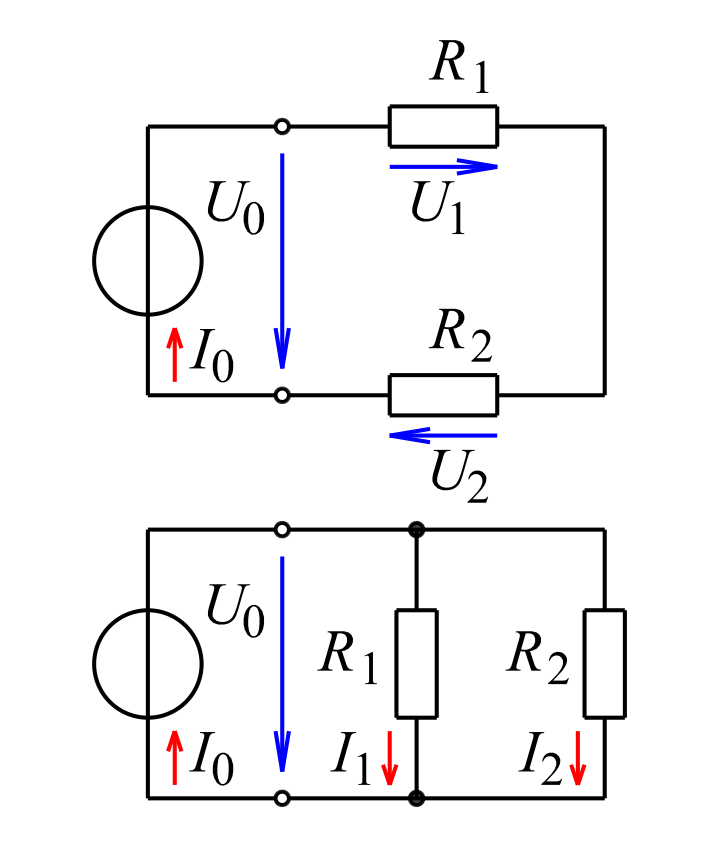
\includegraphics[width=\textwidth]{Reihen_parallel_schaltung.png}
\end{center}
\end{column}

\end{columns}

\end{frame}


\begin{frame}
\frametitle{Beispiel für Parallelschaltung im menschlichen Körper?}

\pause

Glomerulus in der Niere:

\begin{center}
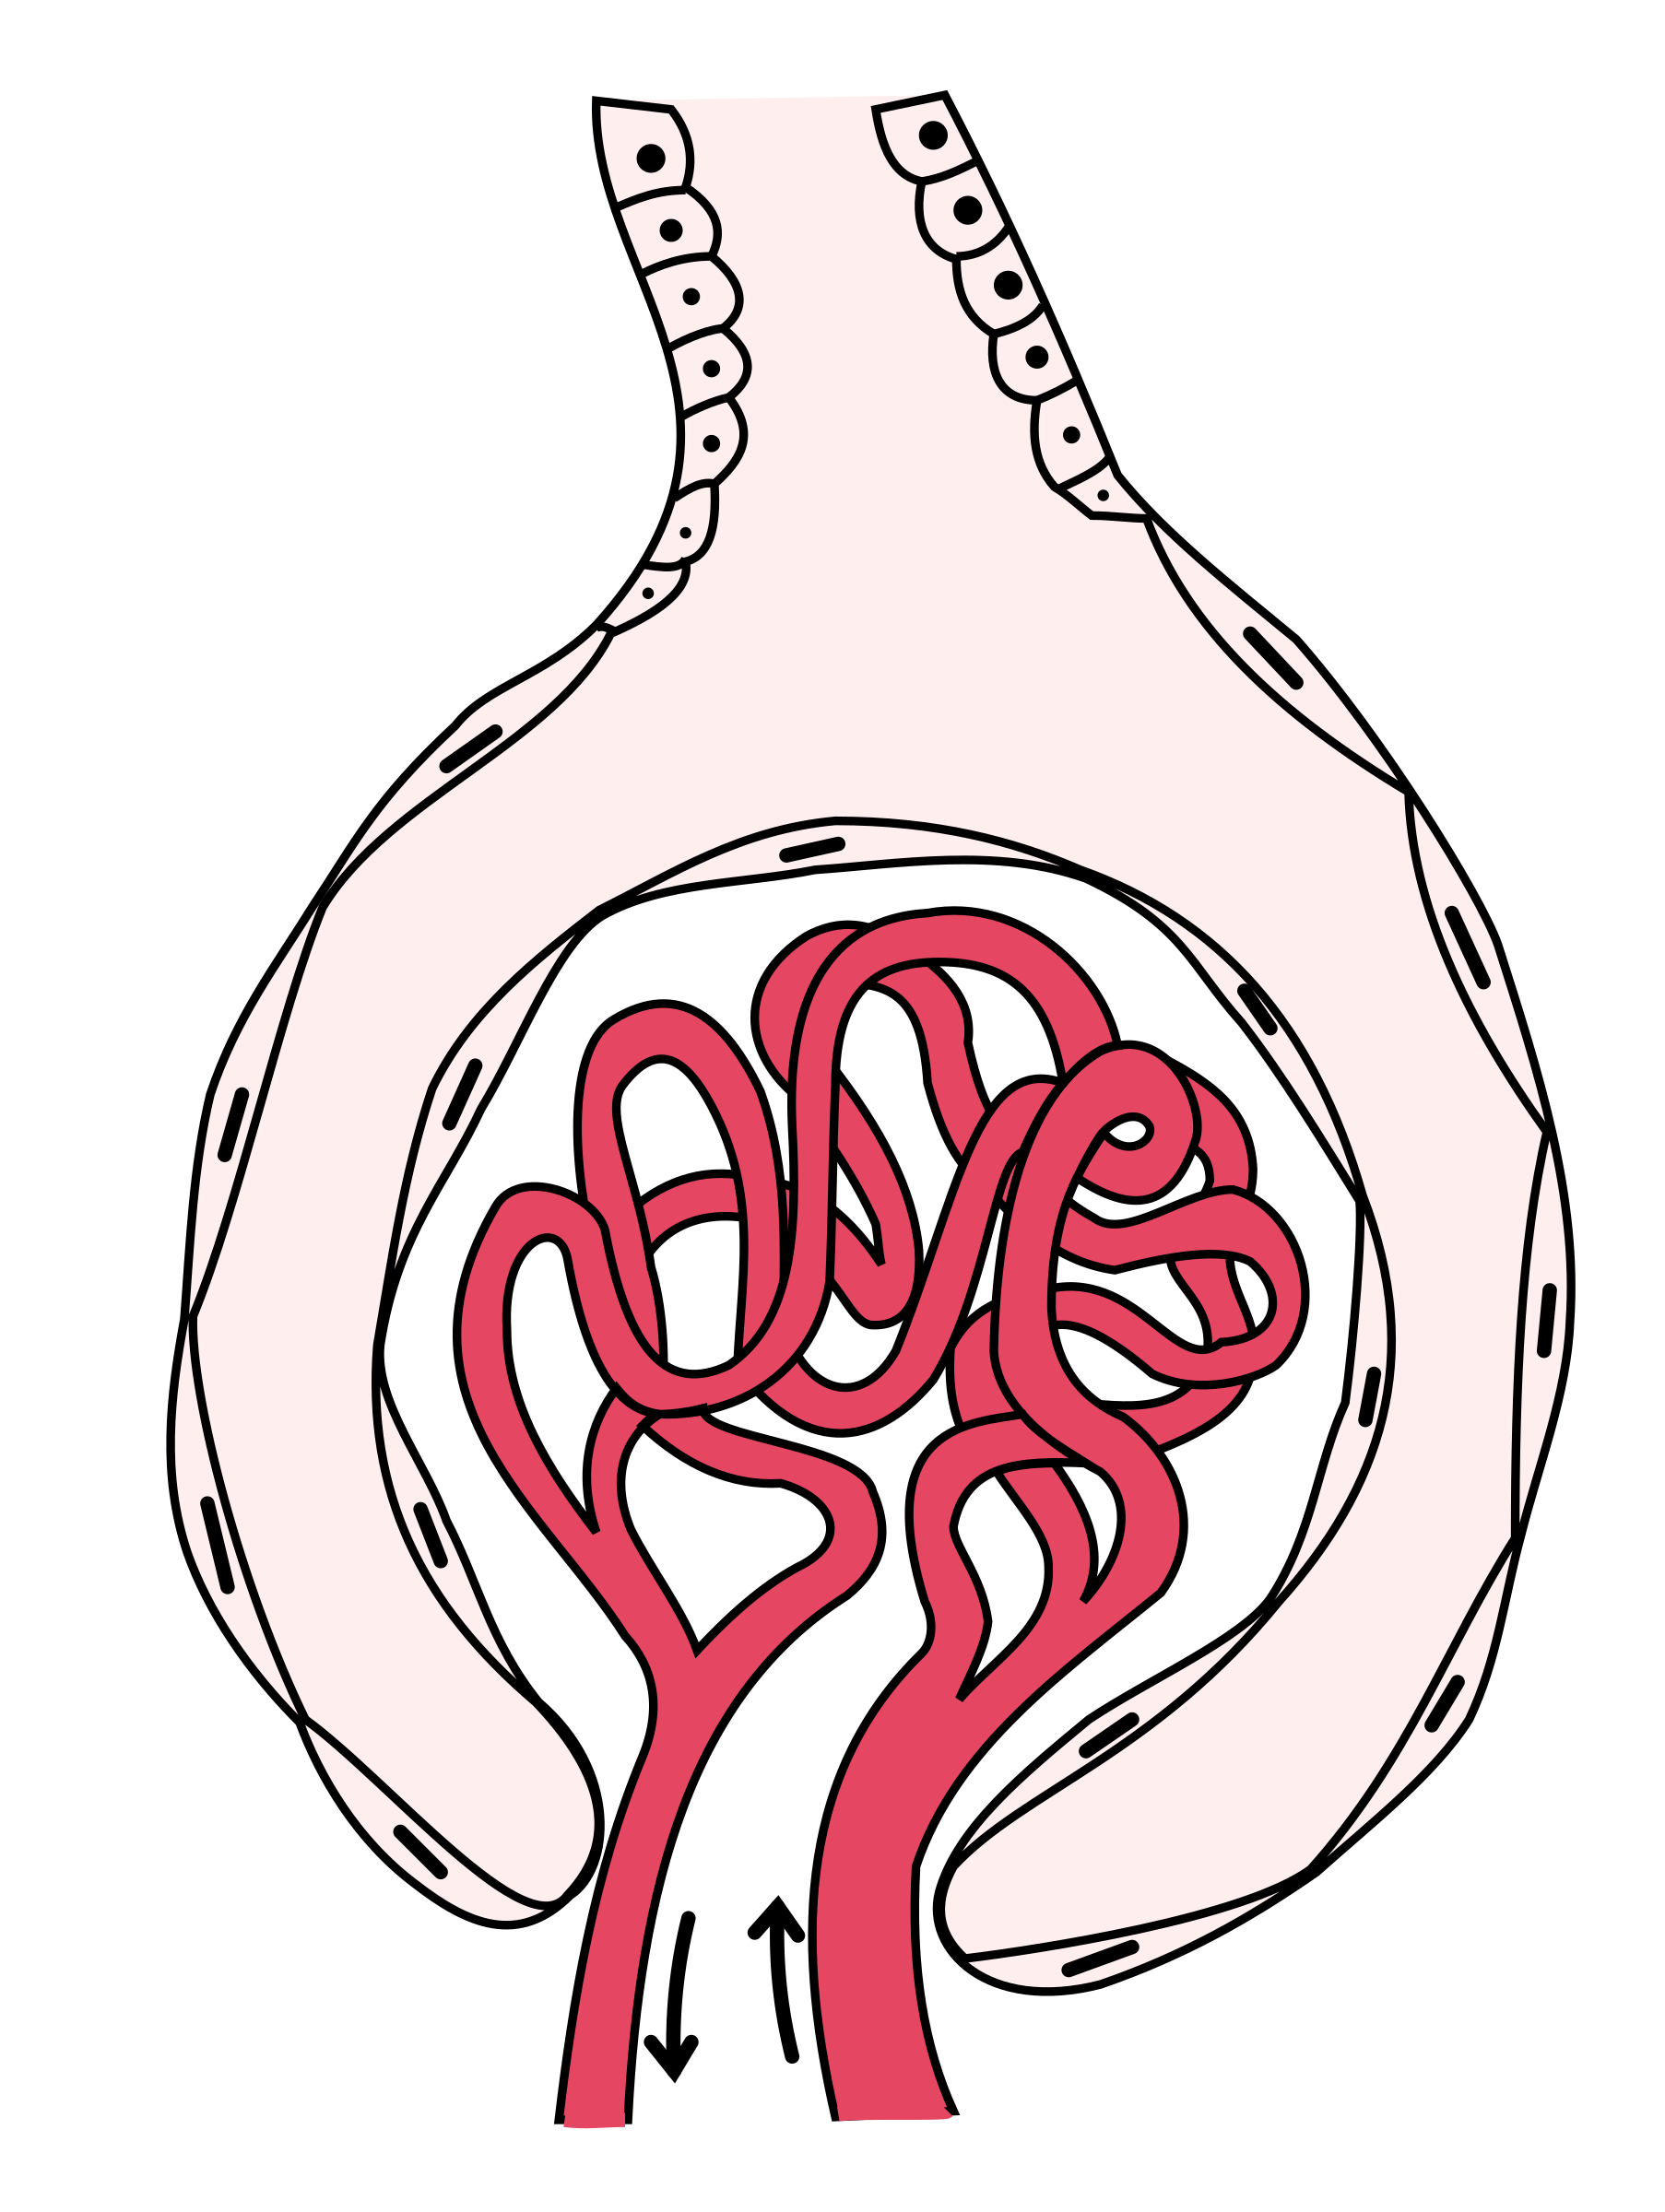
\includegraphics[width=0.4\textwidth]{nierenkoerperchen.png}
\end{center}


\end{frame}





\section{Kräfte an Grenzflächen}



%% - Kohäsion und Adhäsion definieren

\begin{frame}
\frametitle{Kohäsion und Adhäsion}

\begin{columns}[c]

\begin{column}{5cm}
\begin{center}
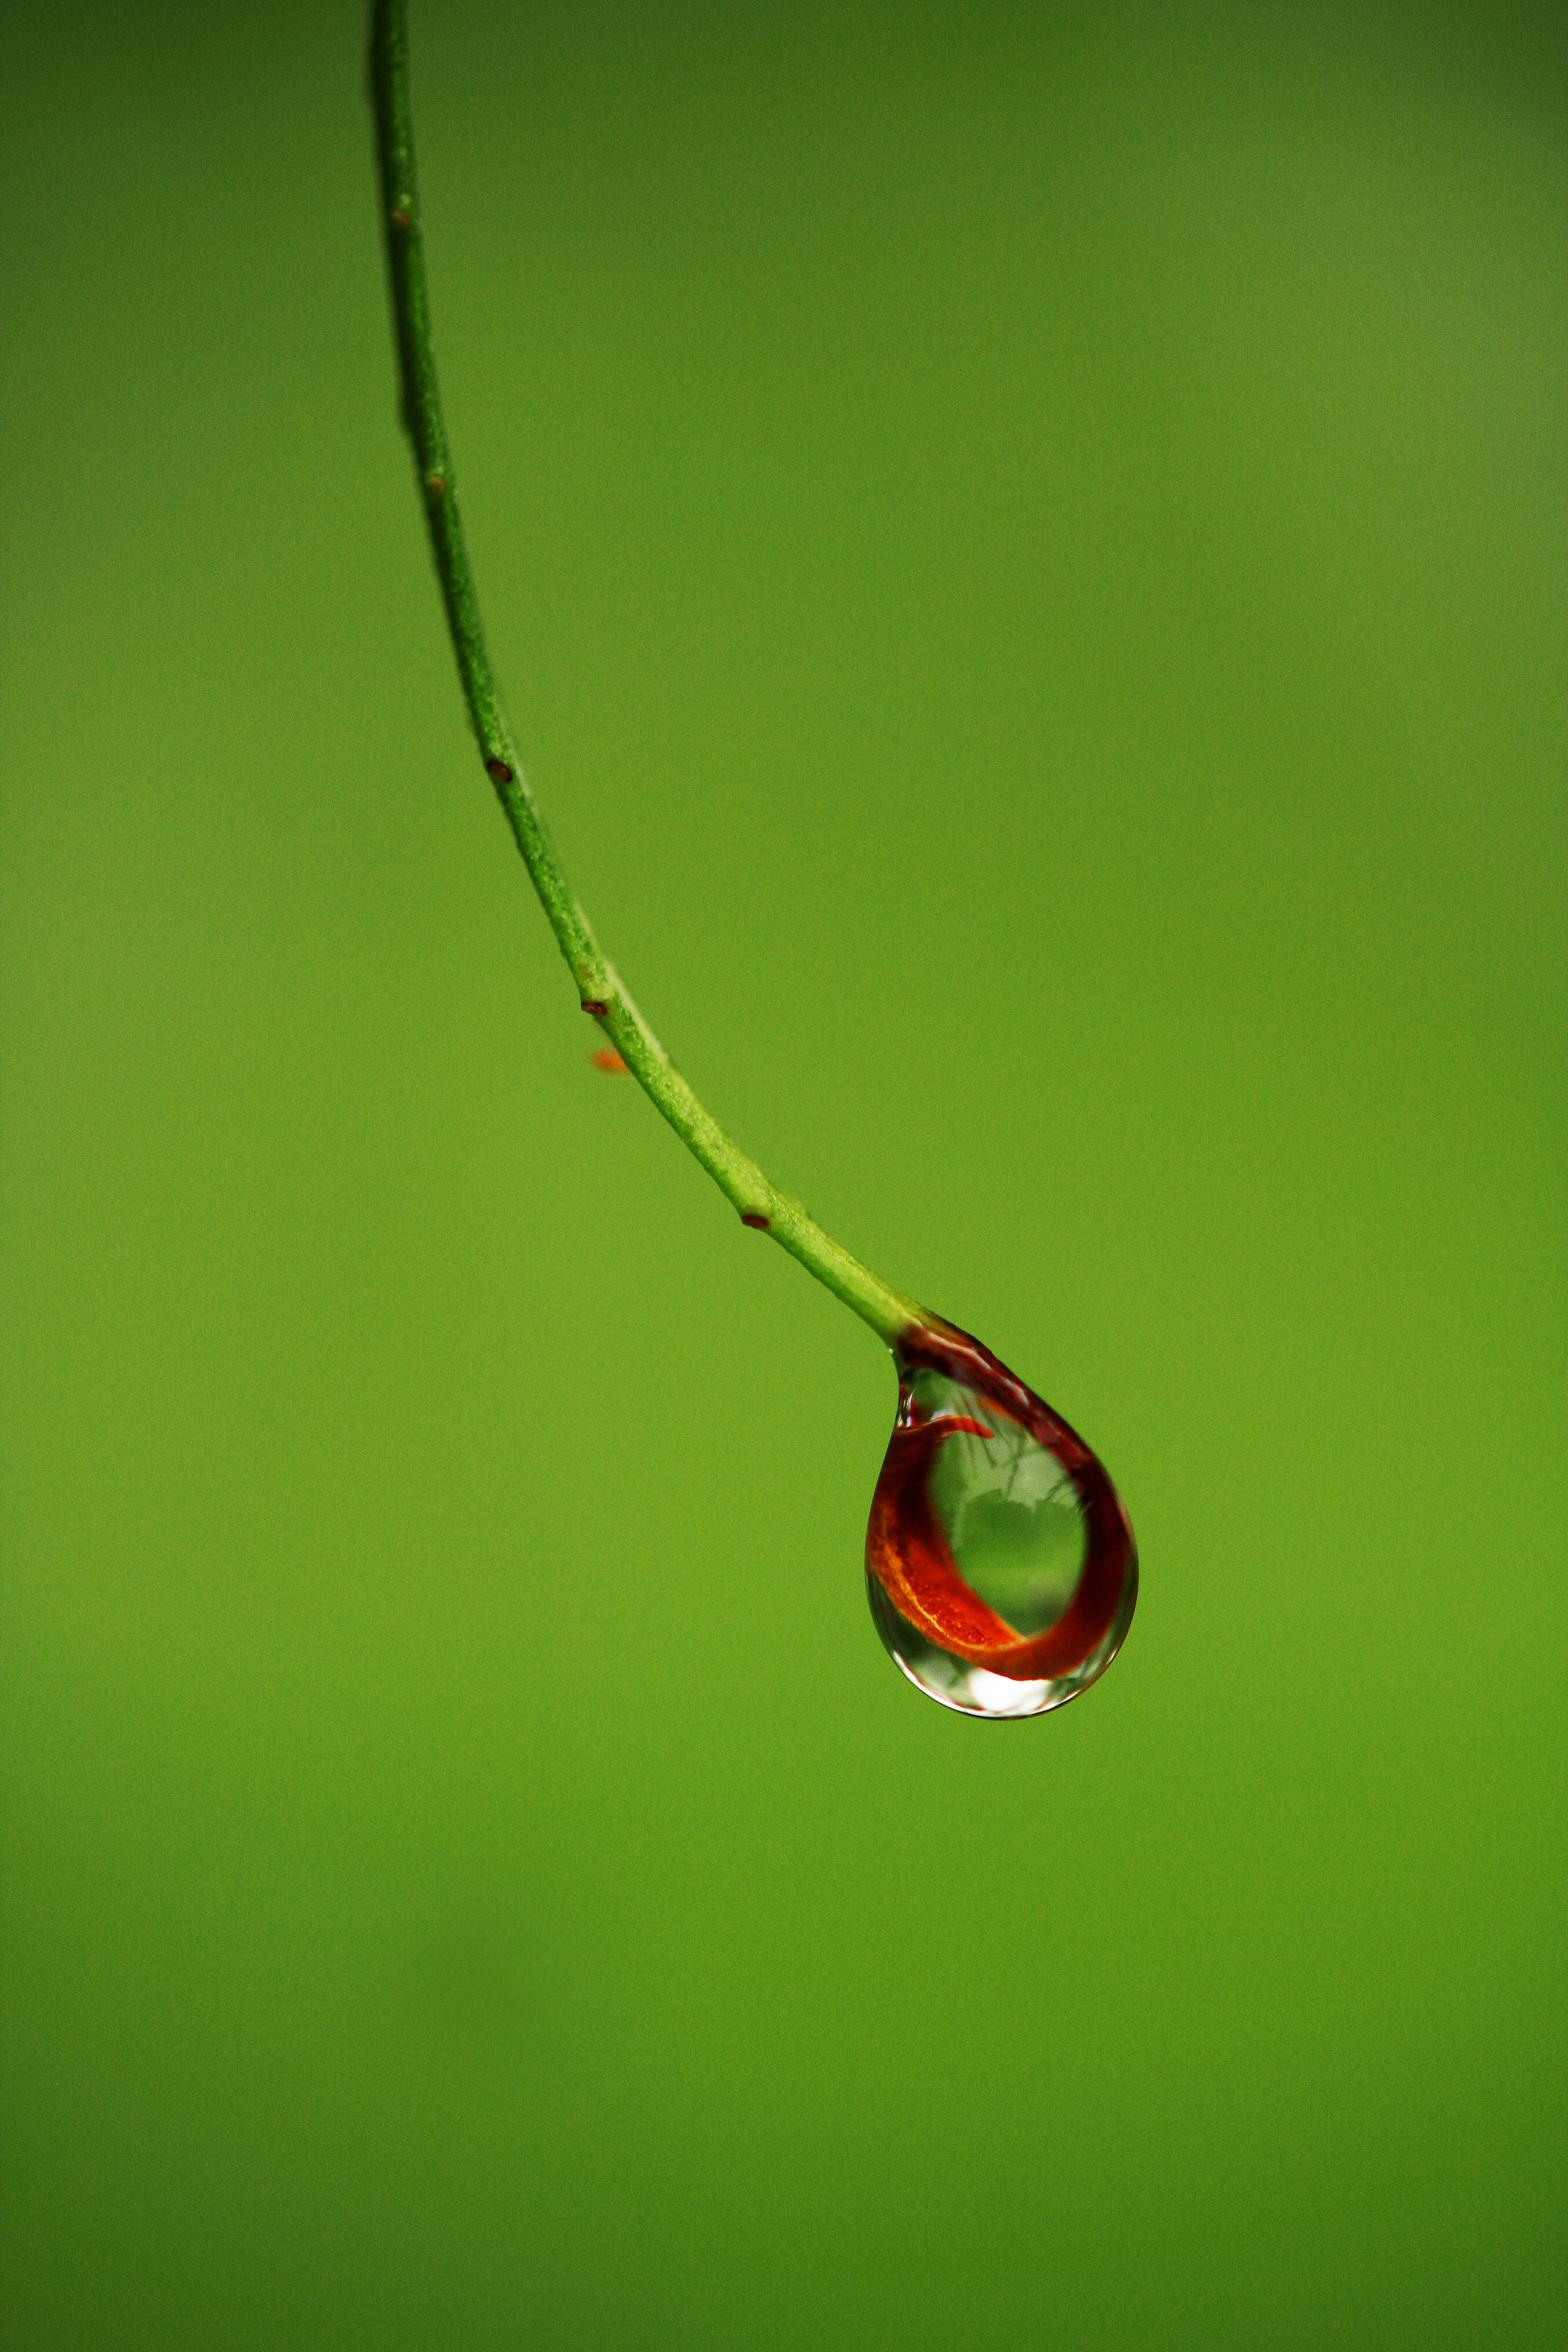
\includegraphics[width=\textwidth]{drop.jpg}
\end{center}

\end{column}

\begin{column}{5cm}

\begin{block}{Kohäsion}

Zusammenhalt/Bindung zwischen Molekülen \textbf{desselben} Stoffes

\end{block}

\begin{block}{Adhäsion}

Zusammenhalt/Bindung zwischen Molekülen \textbf{verschiedener} Stoffe

\end{block}

\end{column}

\end{columns}

\end{frame}


\begin{frame}
\makebox[\linewidth]{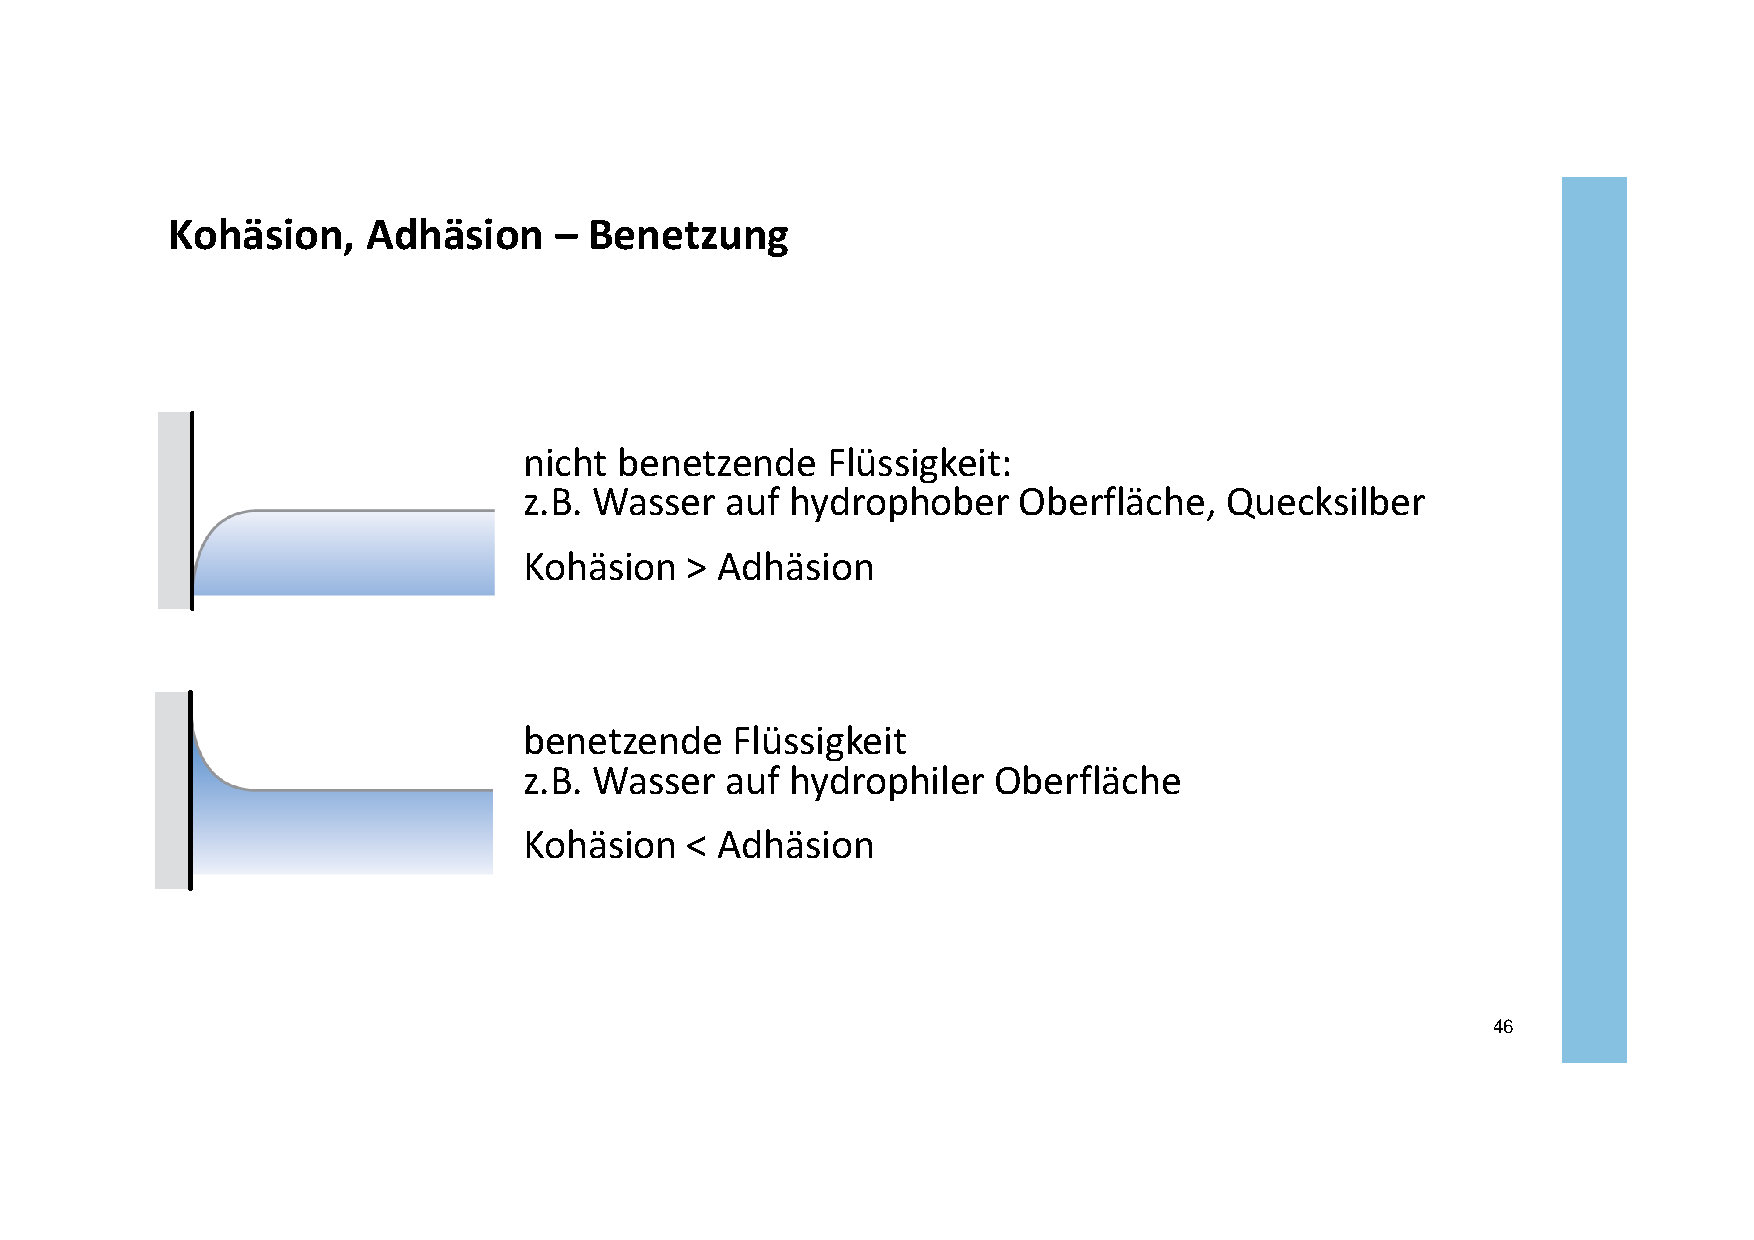
\includegraphics[width=\textwidth]{Walter_Druck_Benetzung.pdf}}
\end{frame}


%% - Den Kapillareffekt erklären und Beispiele geben

\begin{frame}
\frametitle{Kapillareffekt - vereinfachte Anschauung}

\begin{center}
\includegraphics<1>[width=\textwidth]{kapillare_1.png}
\includegraphics<2>[width=\textwidth]{kapillare_2.png}
\includegraphics<3>[width=\textwidth]{kapillare_3.png}
\includegraphics<4>[width=\textwidth]{kapillare_4.png}
\end{center}

\end{frame}

\begin{frame}
\makebox[\linewidth]{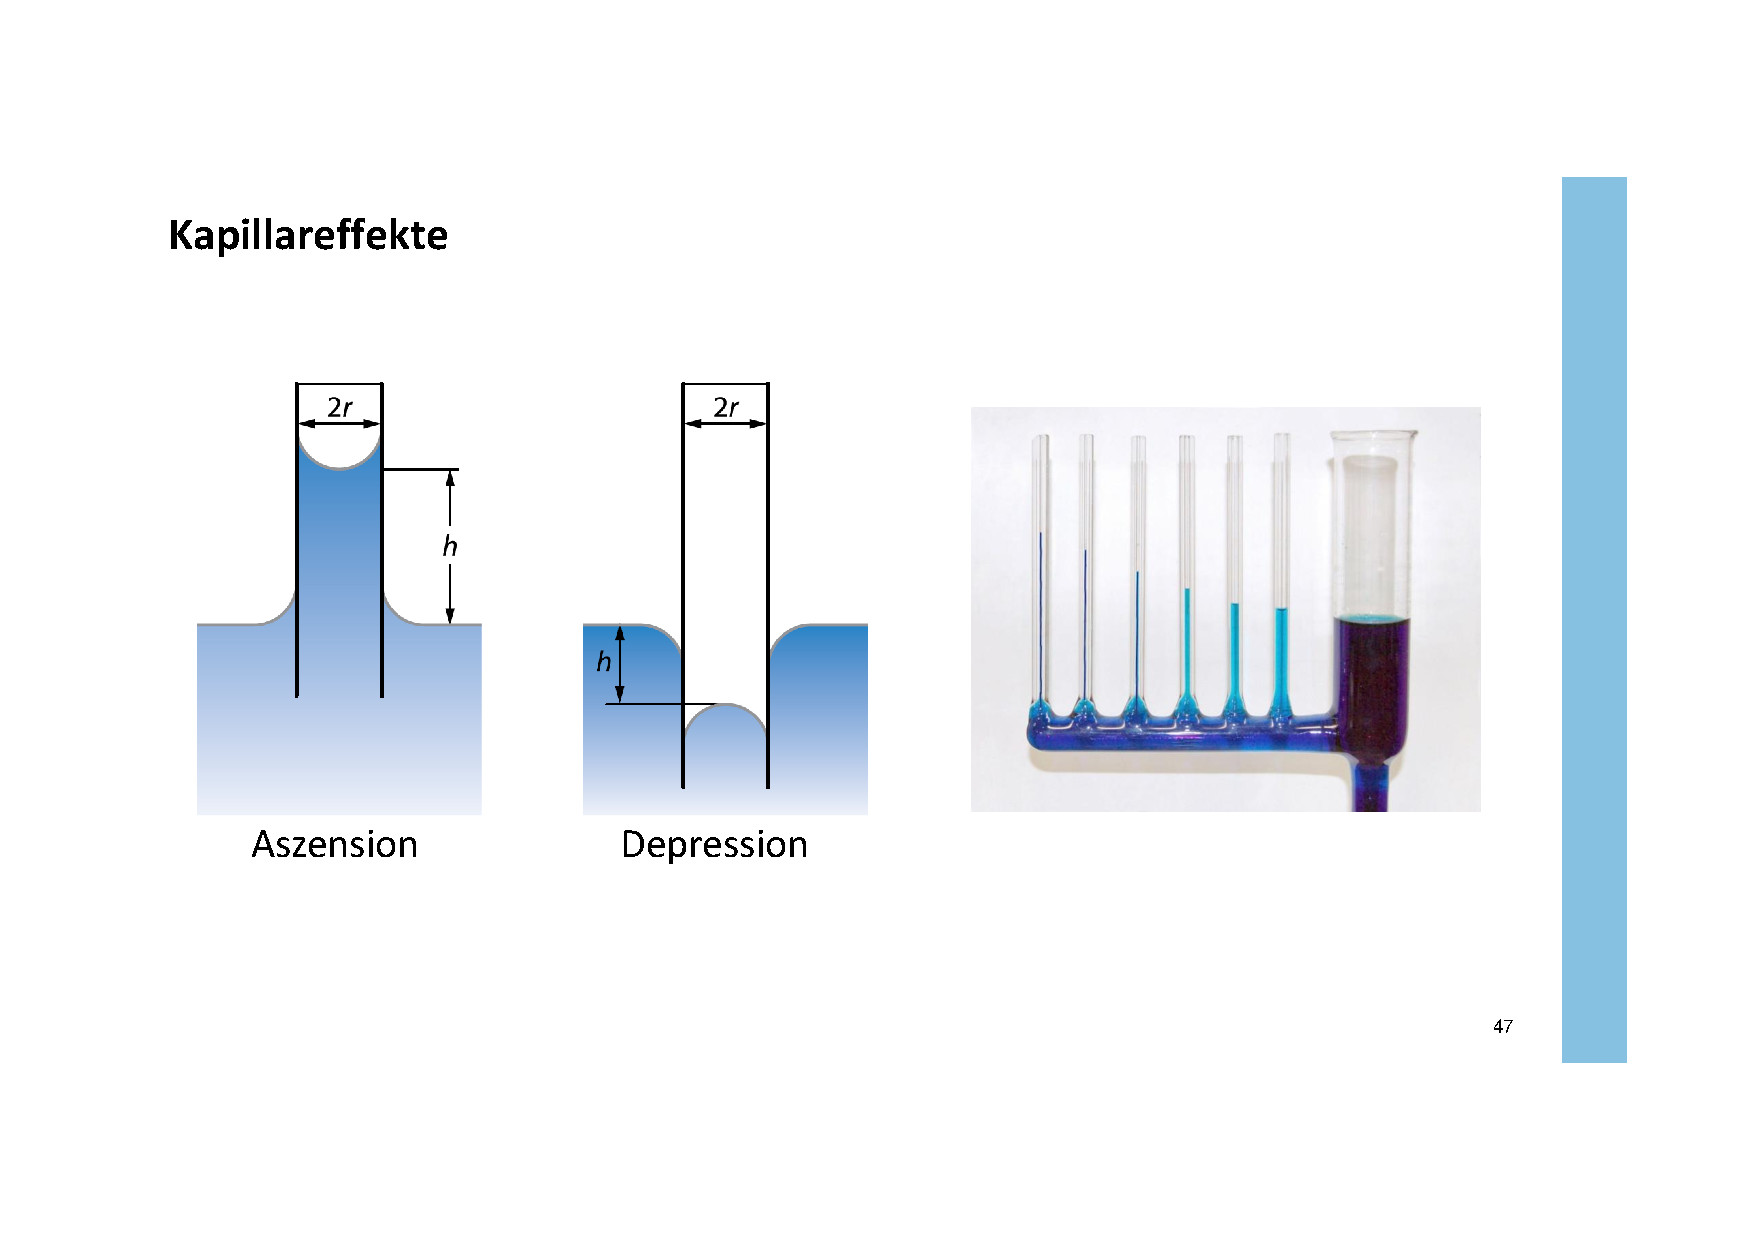
\includegraphics[width=\textwidth]{Walter_Kapillareffekt1.pdf}}
\end{frame}

\begin{frame}
\makebox[\linewidth]{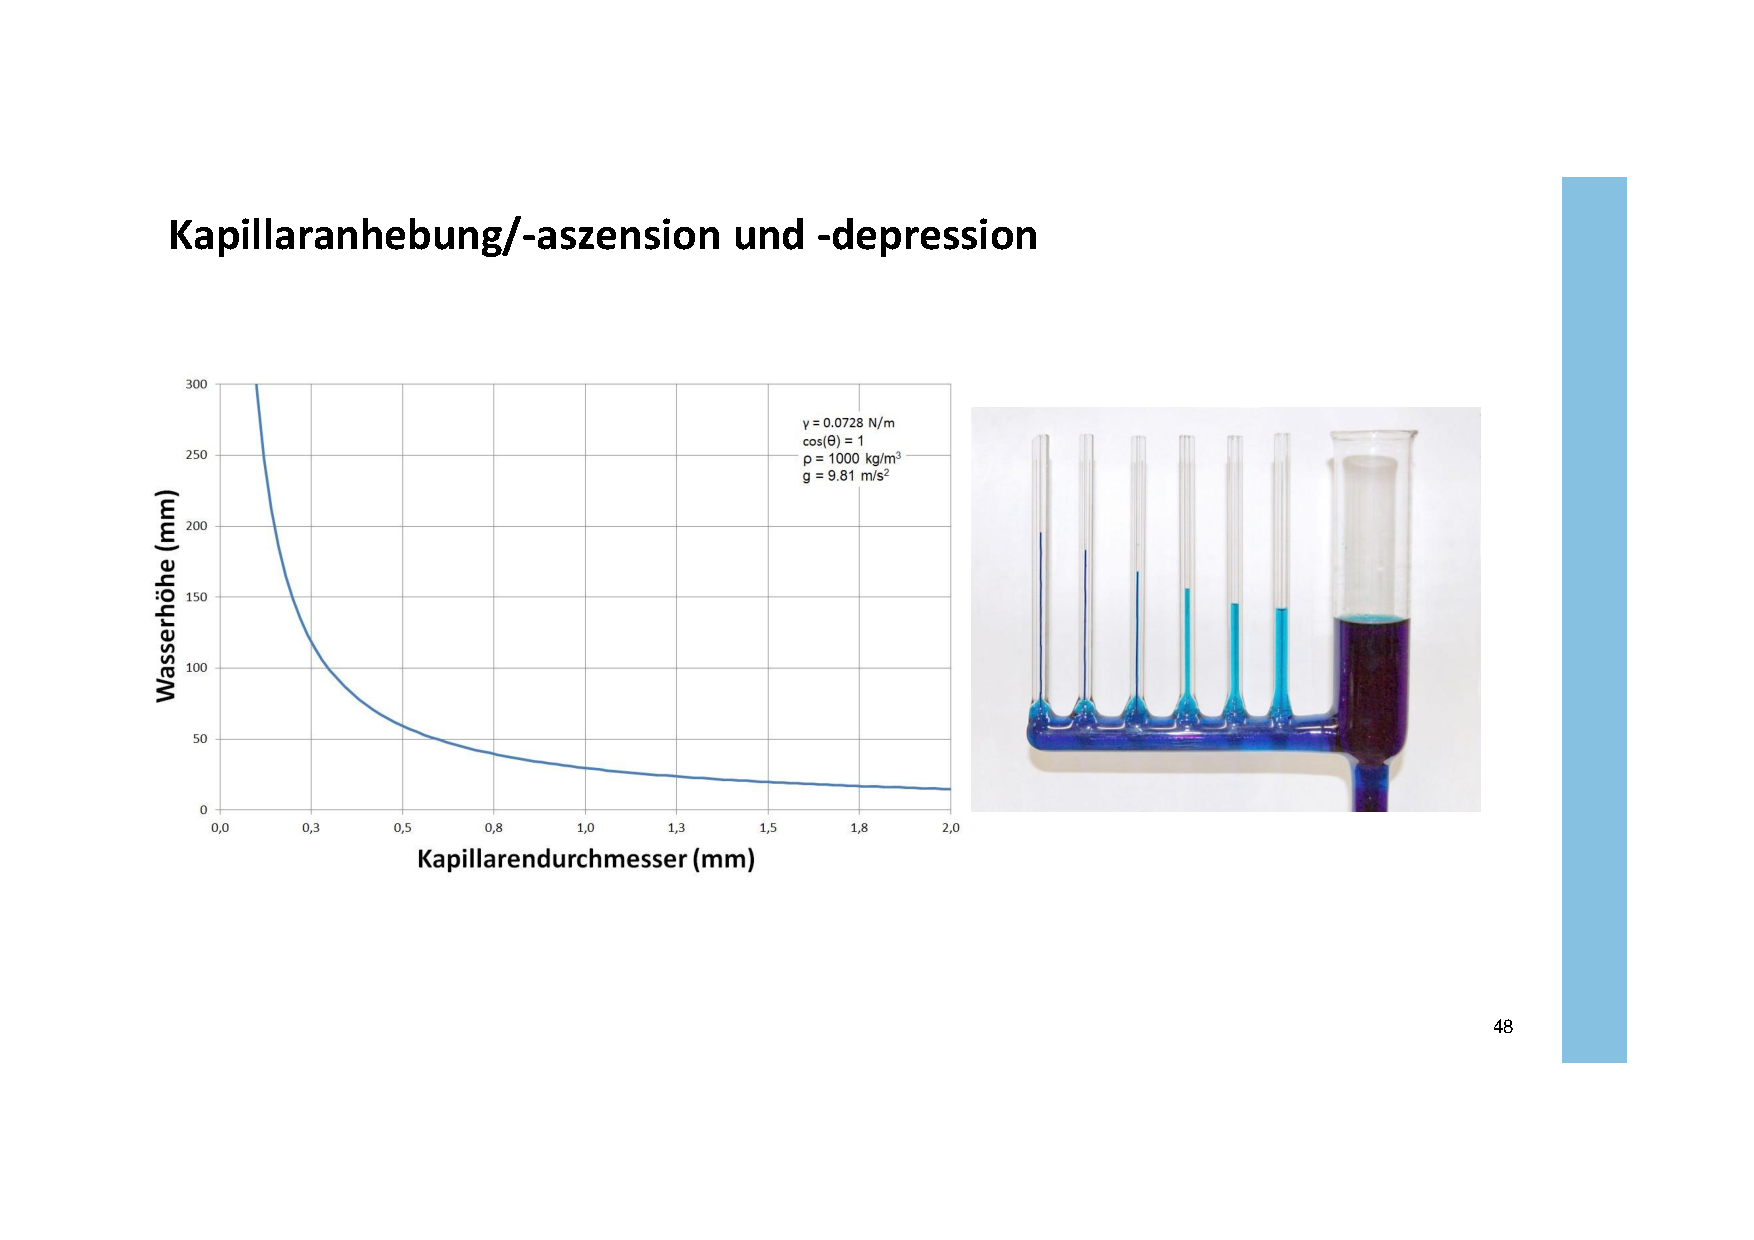
\includegraphics[width=\textwidth]{Walter_Kapillareffekt2.pdf}}
\end{frame}


%% Kapillareffekt: Beispiel Covid test

\begin{frame}
\frametitle{Beispiel: Lateral flow test}

\begin{center}
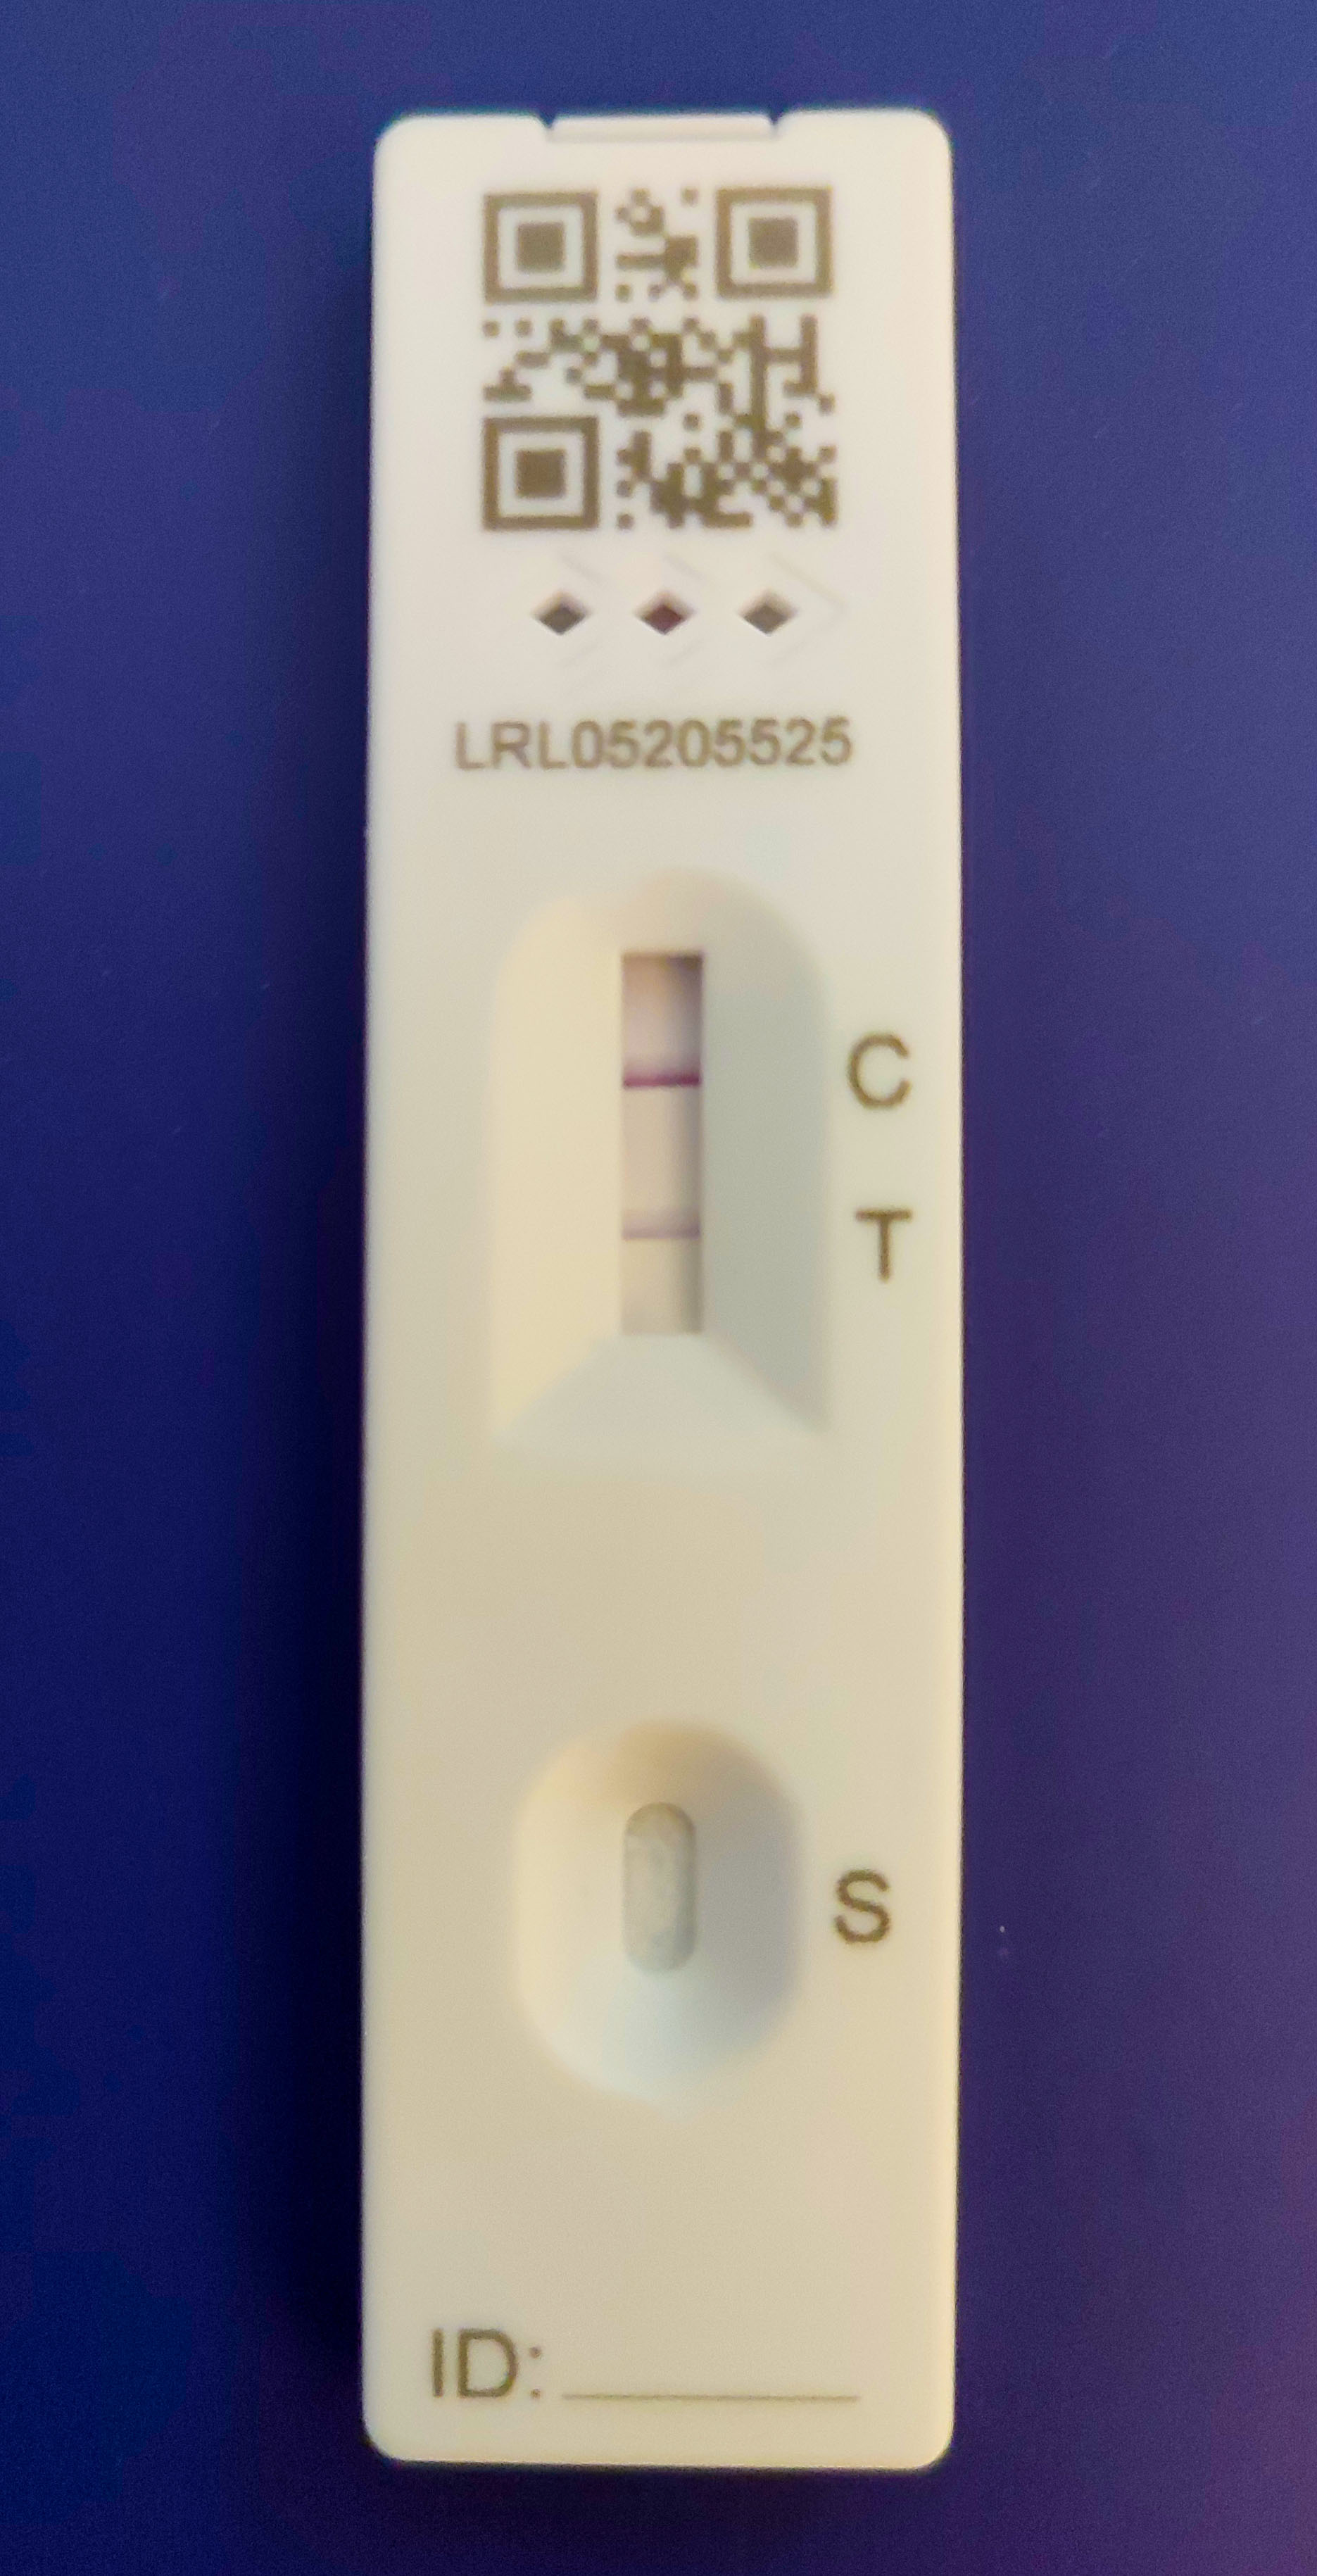
\includegraphics[width=0.4\textwidth, angle=-90, origin=c]{covid_test.jpg}
\end{center}

\end{frame}

\begin{frame}
\frametitle{Beispiel: Lateral flow test}

\begin{center}
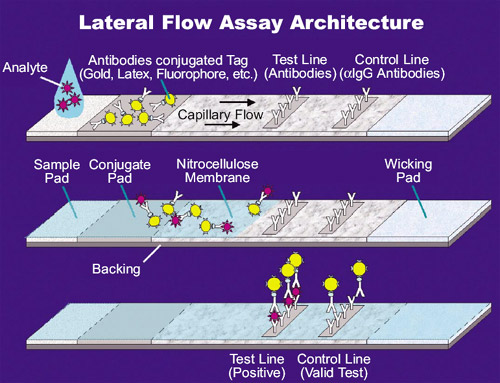
\includegraphics[width=0.8\textwidth]{lateral_flow_test.jpg}
\end{center}

\end{frame}



%% - Oberflächenspannung definieren
\begin{frame}
\frametitle{Oberflächenspannung}

\begin{columns}[c]

\begin{column}{5cm}
\begin{center}
\includegraphics<1>[width=\textwidth]{cohesion.png}
\includegraphics<2>[width=\textwidth]{seifenblasen.jpg}
\end{center}


\end{column}


\begin{column}{5cm}

Flüssigkeiten wollen* ihre Oberfläche minimieren. 

\pause 
\vfill

(* Es ist energetisch günstiger)



\end{column}


\end{columns}

\end{frame}


%% Oberflächenspannung
\begin{frame}
\frametitle{Oberflächenspannung}

\[
\sigma = \frac{W_A}{A} \qquad \text{Einheit: } \frac{J}{m^2}
\]

\begin{tabular}{ll}
\(\sigma\)      & Oberflächenspannung   \\
\(W_A\)         & Oberflächenenergie    \\
\(A\)           & Oberfläche           \\

\end{tabular}


\end{frame}

%% - Erklären, warum Händewaschen in einer viralen Pandemie wichtig ist

\begin{frame}
\frametitle{Phospholipide in Wasser}

\begin{columns}[c]
\begin{column}{5cm}
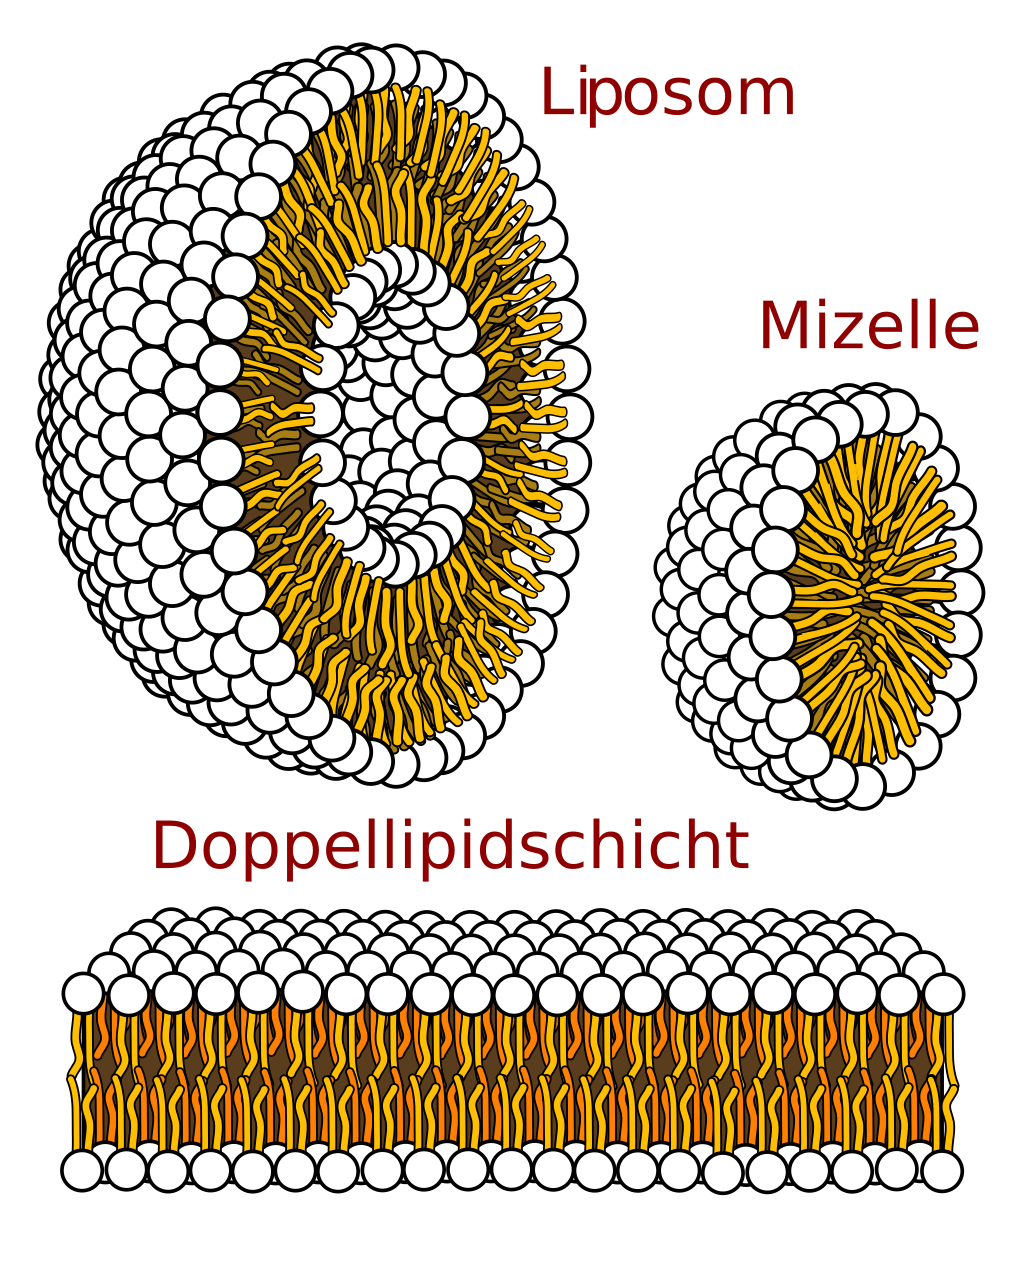
\includegraphics[width=\textwidth]{Phospholipide_in_Wasser.png}
\end{column}

\pause

\begin{column}{5cm}
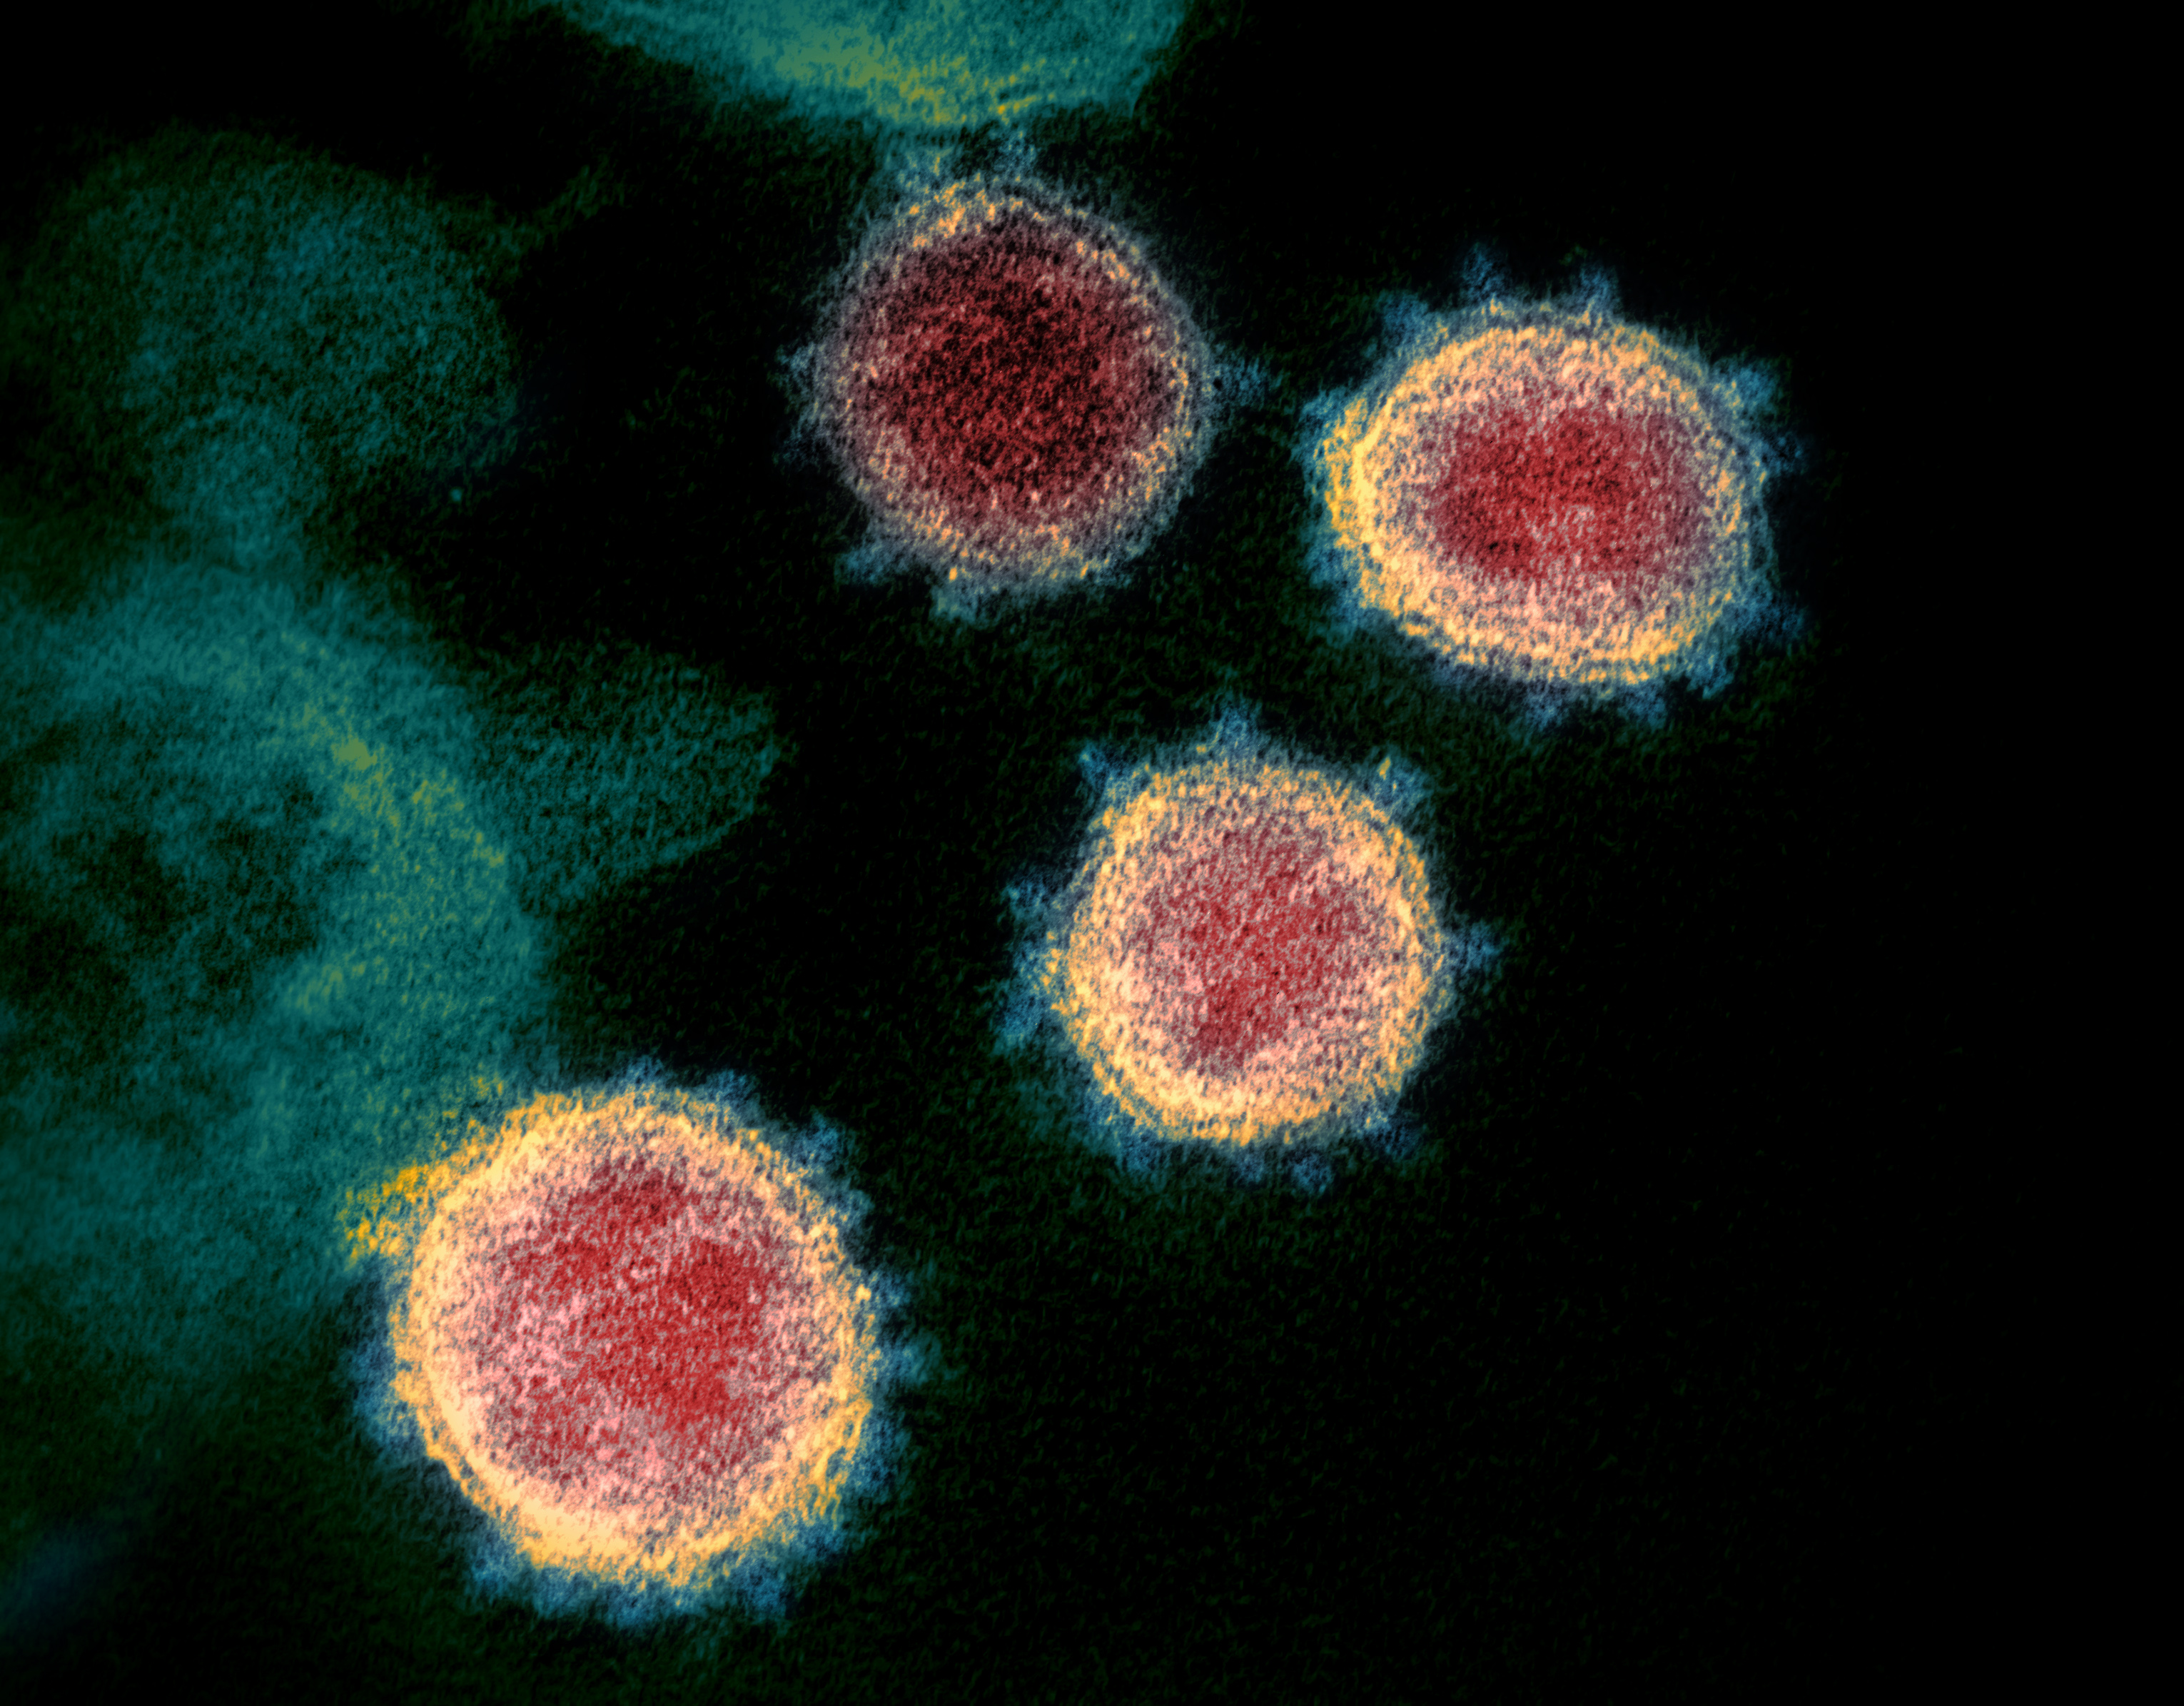
\includegraphics[width=\textwidth]{SARS-CoV-2.jpg}
\end{column}

\end{columns}


\end{frame}

\begin{frame}
\frametitle{Warum hilft Seife?}

\begin{center}
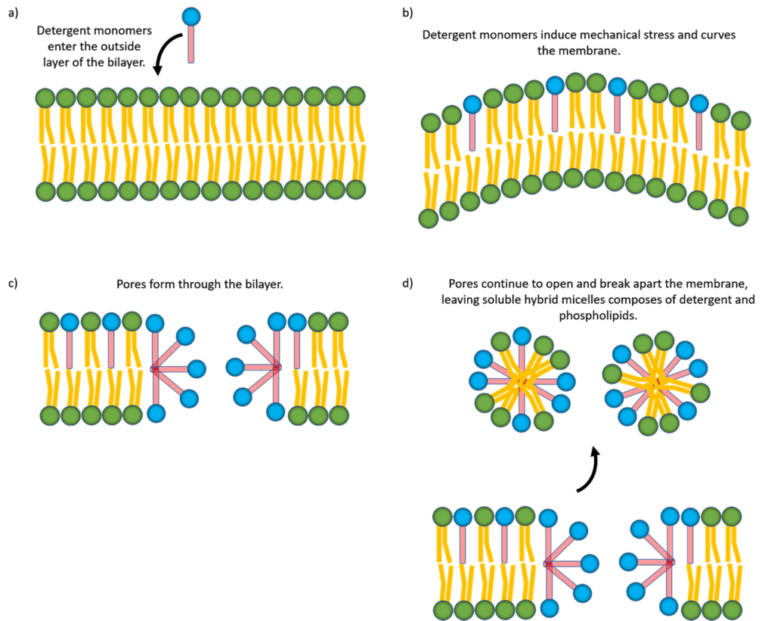
\includegraphics[width=0.8\textwidth]{soap_action.png}
\end{center}

\end{frame}




%% Review

\begin{frame}

\frametitle{Jetzt* sollten Sie:}



\begin{block}{Wissen:}
\begin{itemize}
%%%%%
\item
Eigenschaften von Flüssigkeiten und Gasen erklären
\item
Druck definieren, Stempeldruck erklären
\item
Luftdruck erklären 
\item
Schweredruck in Flüssigkeiten und Auftrieb erklären
\item
Auswirkungen von Druck auf den menschlichen Organismus erklären
%%%%%
\item
Volumenstrom, Strömungswiderstand, Strömungsleitwert definieren 
\item
Kontinuitätsgleichung kennen 
%%%%%
\item
Kohäsion und Adhäsion definieren
\item
Den Kapillareffekt erklären und Beispiele geben
\item
Oberflächenspannung definieren
\end{itemize}

\end{block}

\end{frame}

\begin{frame}

\frametitle{Jetzt* sollten Sie:}
 



\begin{block}{Können:}
\begin{itemize}
\item
Druck und Auftrieb berechnen
\item
Luftdruck an verschiedenen Orten abschätzen
\item
Schweredruck im Wasser abschätzen
%%%%%%%
\item
Volumenstrom, Strömungswiderstand, Strömungsleitwert berechnen
\item
Die Kontinuitätsgleichung anwenden
\item
Strömungsfelder durch Stromlinien darstellen
\item
Prinzipien der Strömung im Blutkreislauf und in der Atmung erkennen
\item
Den Bernoulli-Effekt mit Alltagsgegenständen demonstrieren
\item
Die Kirchhoff-Gesetze anwenden
\item
Das Hagen-Poiseuille Gesetz anwenden
%%%%%%%
\item
Erklären, warum Händewaschen in einer viralen Pandemie wichtig ist
\end{itemize}
\end{block}

\end{frame}

\begin{frame}

\frametitle{Jetzt* sollten Sie:}
 

\begin{columns}[c]

\begin{column}{7cm}
\begin{block}{Fühlen:}

\begin{itemize}
\item
Die eigene Intuition im Hinblick auf Flüssigkeiten und Gase hinterfragen
\item
Die Augen offen halten für hydrodynamische und aerodynamische Effekte im Alltag und in der Medizin
\end{itemize}

\end{block}

\end{column}

\begin{column}{4cm}
\begin{center}
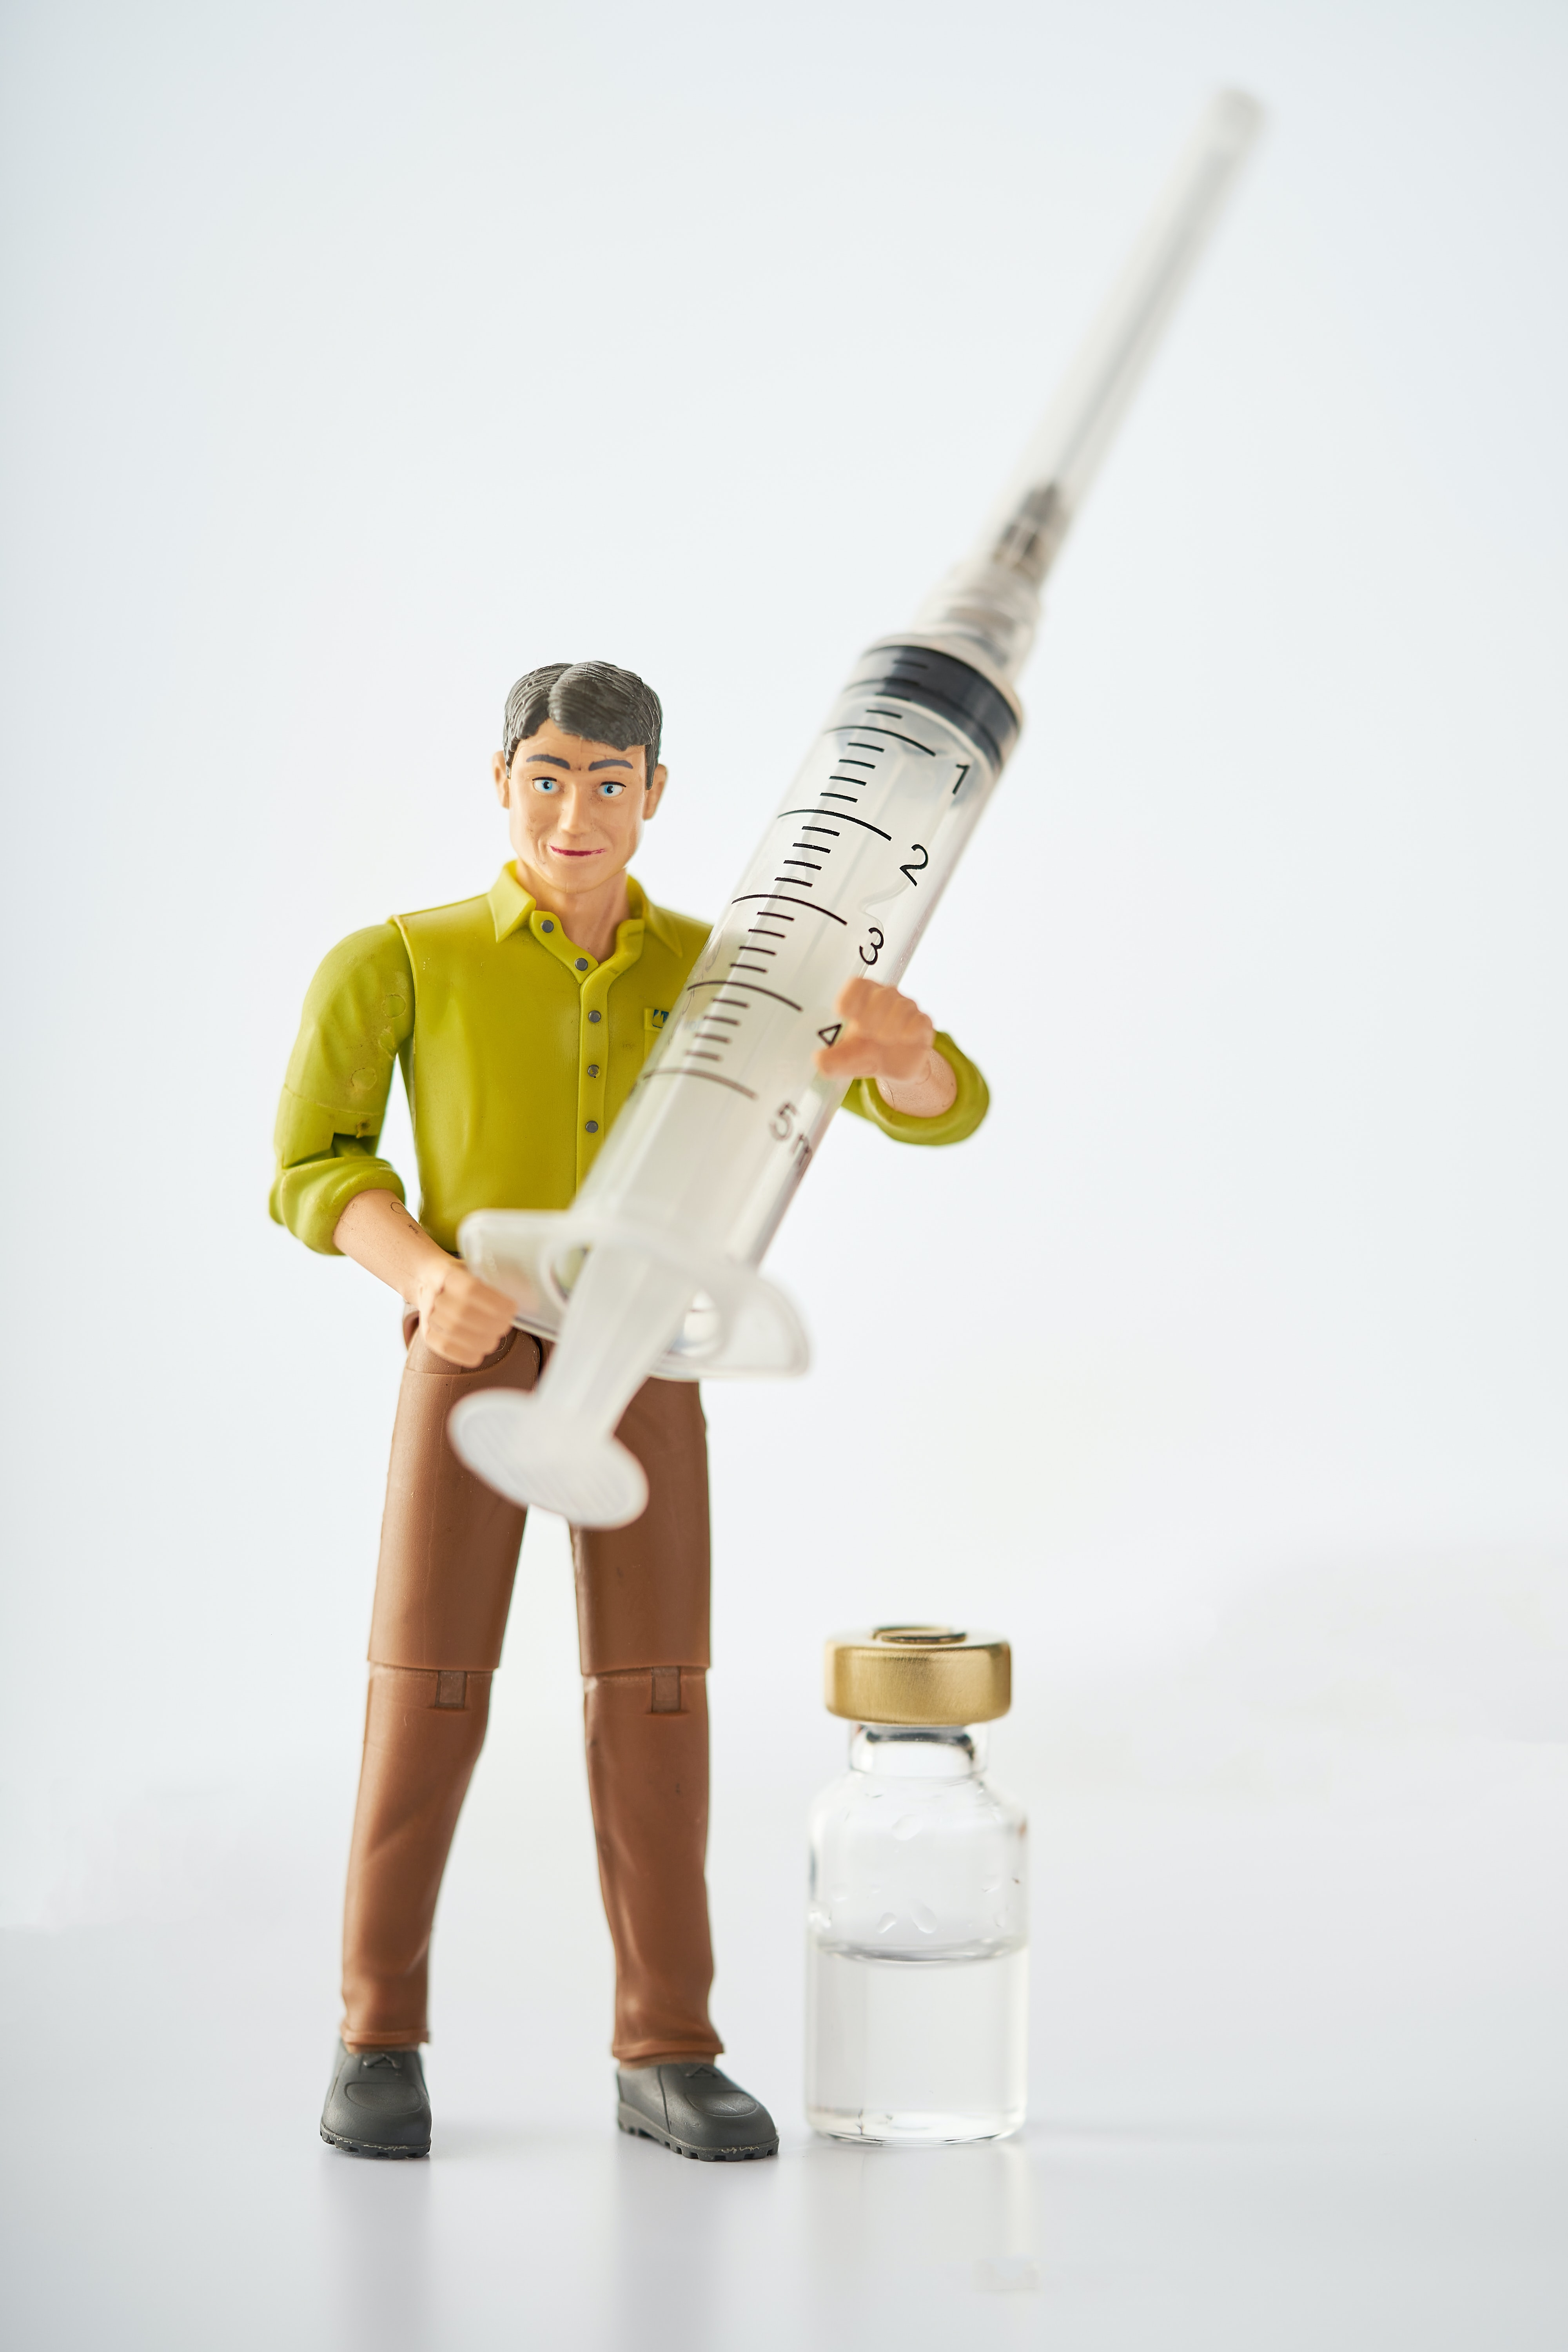
\includegraphics[width=\textwidth]{action_figure_needle.jpg}
\end{center}

\end{column}
\end{columns}



 \end{frame}








\begin{frame}
\frametitle{Danke für Ihr Feedback!}

\begin{columns}[c]

\begin{column}{6cm}
\begin{center}
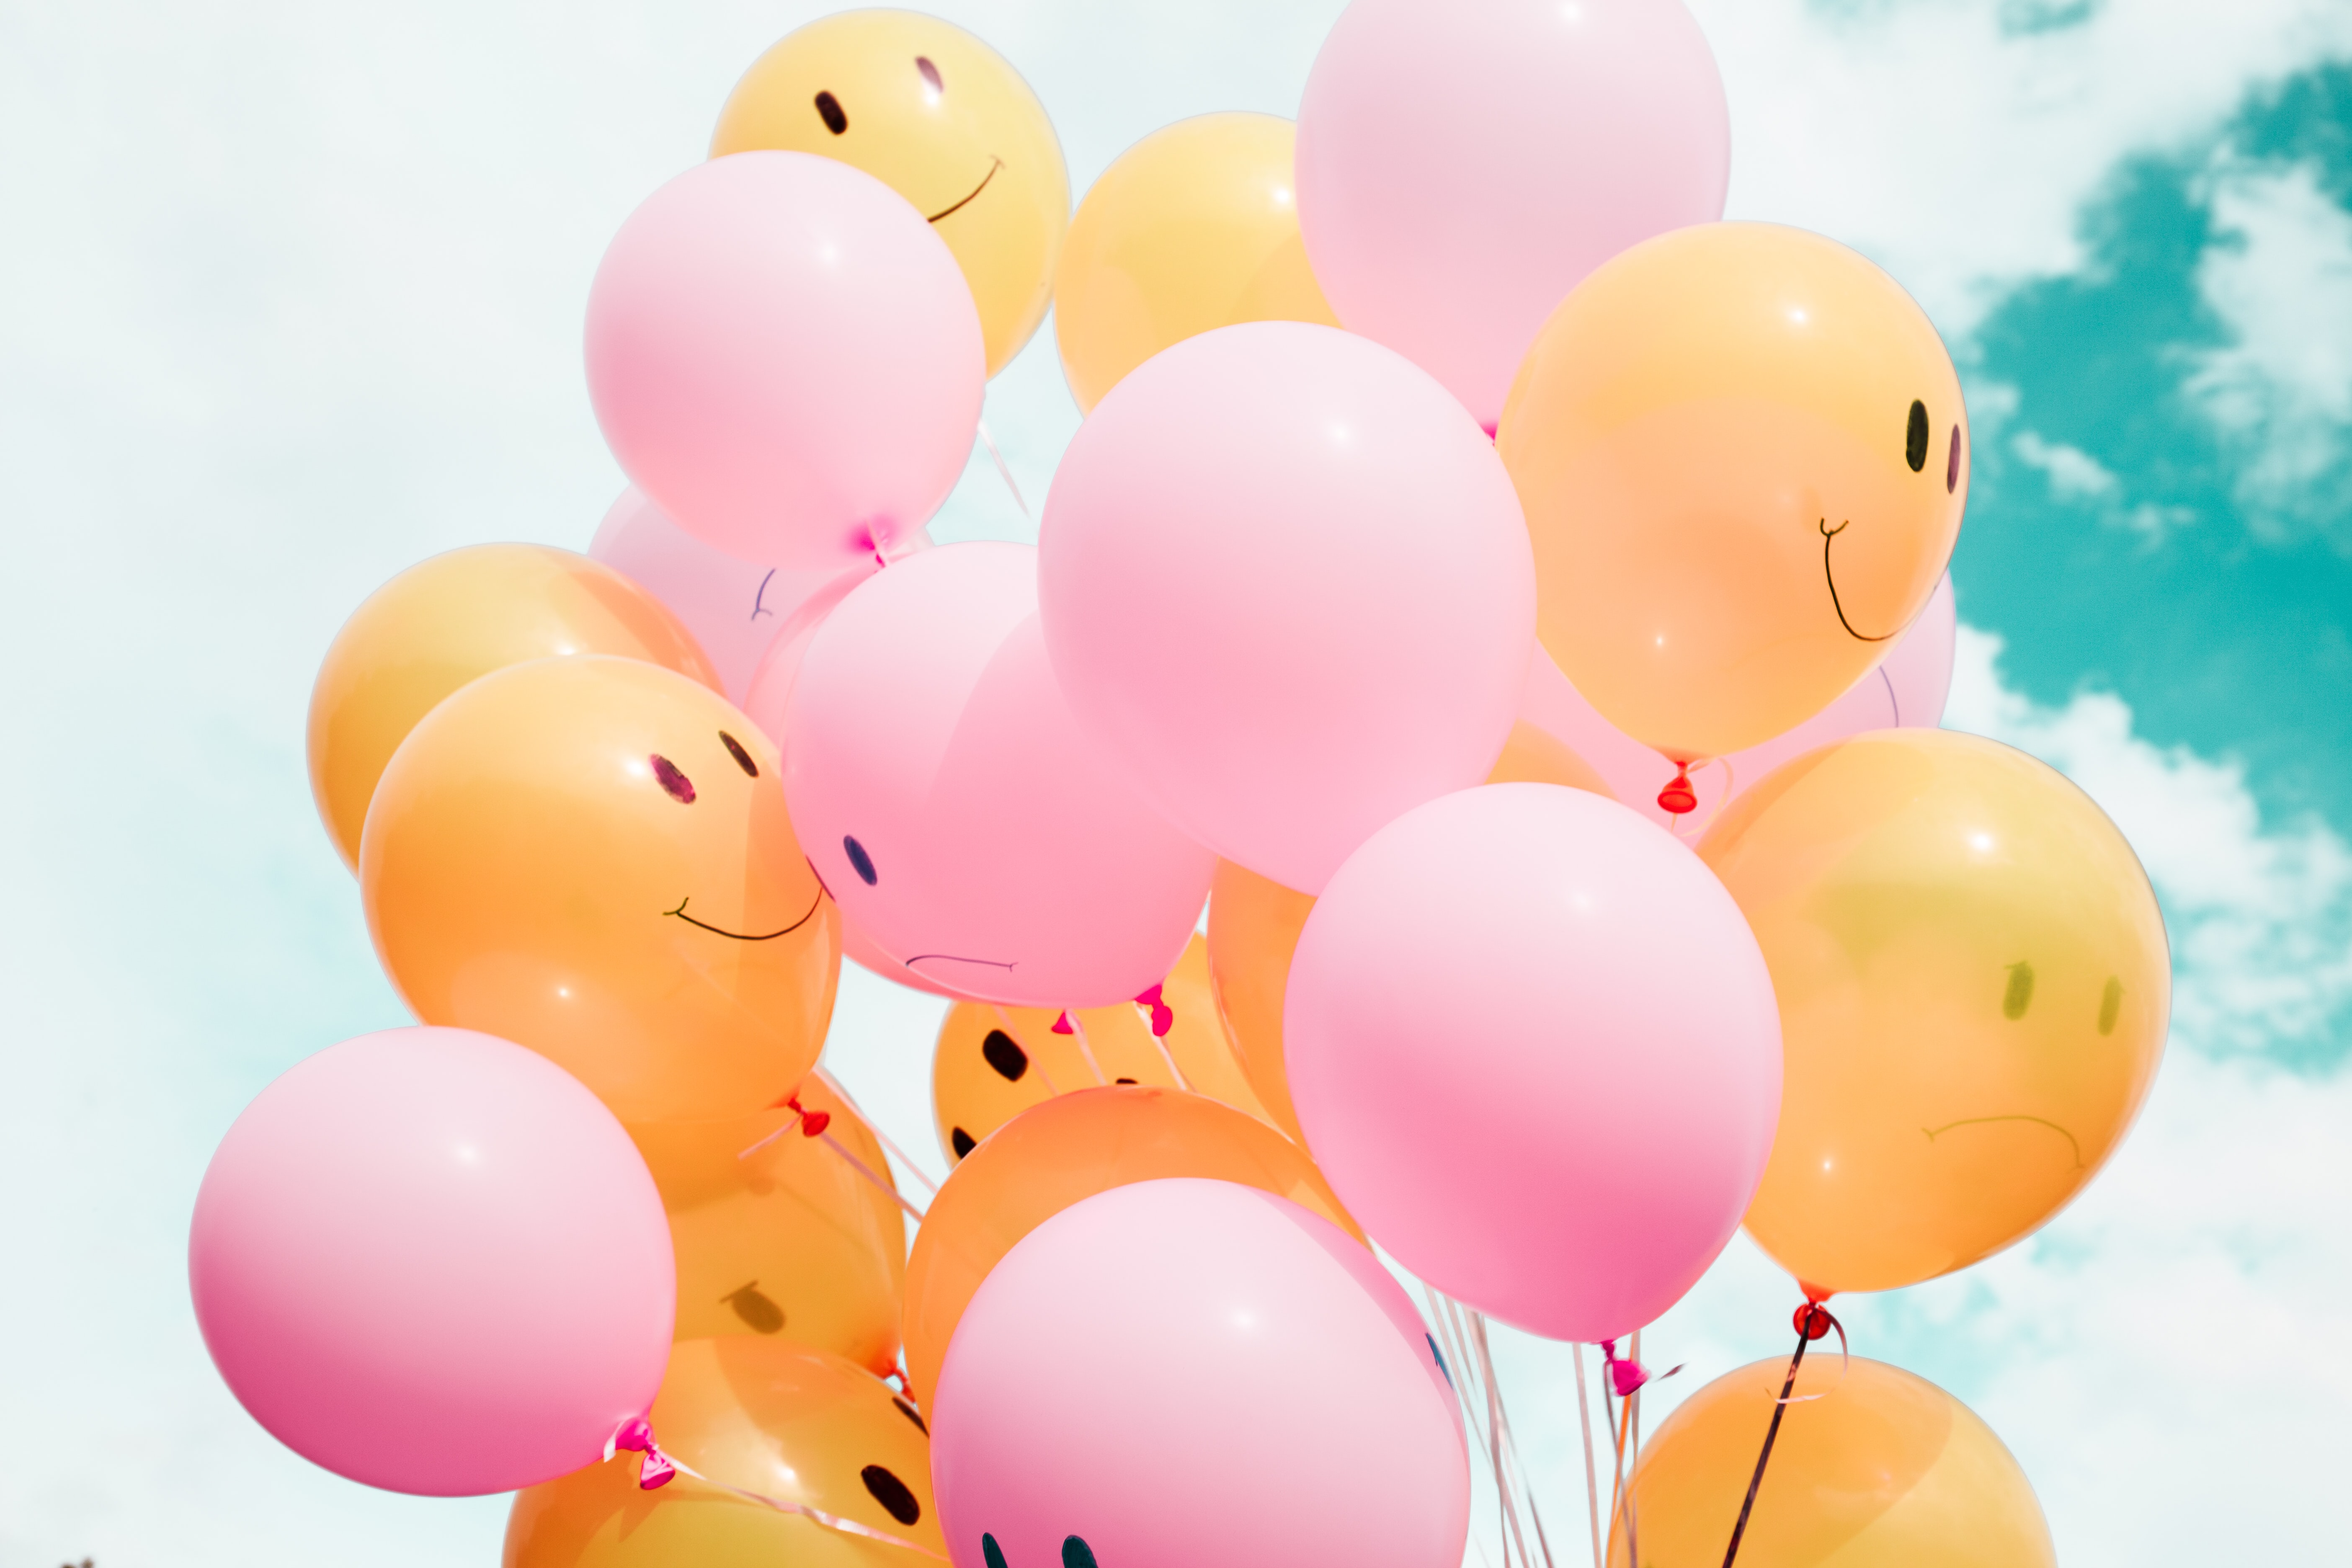
\includegraphics[width=\textwidth]{smilie_balloons.jpg}
\end{center}

\end{column}

\begin{column}{4cm}


\begin{center}

\includegraphics[width=\textwidth]{feedback_QR.png}
\end{center}
\end{column}


\end{columns}

\end{frame}





%% Bildnachweis
\begin{frame}
\frametitle{Bildnachweis}
\begin{tiny}
Diese Vorlesung verwendet teilweise Materialien (Folien und Bilder) einer früheren Vorlesung von Prof. Wim Walter.  Wo nicht anders nachgewiesen, sind auch Bilder aus dieser Vorlesung. 
\end{tiny}

\vfill

\begin{tiny}
 
\begin{itemize}

\item
Action figure mit einer Injektionsspritze. Photo by \href{https://unsplash.com/@manuelchinchilla?utm_source=unsplash&utm_medium=referral&utm_content=creditCopyText}{Manuel Chinchilla} on \href{https://unsplash.com/s/photos/injection?utm_source=unsplash&utm_medium=referral&utm_content=creditCopyText}{Unsplash}

\item
Blutspende. Von Reytan - Eigenes Werk, Gemeinfrei, \url{https://commons.wikimedia.org/w/index.php?curid=388382}

\item
Covid-Schnelltest. Iantresman, CC BY-SA 4.0 \url{https://creativecommons.org/licenses/by-sa/4.0}, via Wikimedia Commons
  

\item
Elefant. Photo by \href{https://unsplash.com/@wolfgang_hasselmann?utm_source=unsplash&utm_medium=referral&utm_content=creditCopyText}{Wolfgang Hasselmann} on \href{https://unsplash.com/s/photos/elephant?utm_source=unsplash&utm_medium=referral&utm_content=creditCopyText}{Unsplash}
  
\item
Glühbirne. Photo by \href{https://unsplash.com/@ajoshuamelo?utm_source=unsplash&utm_medium=referral&utm_content=creditCopyText}{Joshua Melo} on \href{https://unsplash.com/s/photos/lightbulb?utm_source=unsplash&utm_medium=referral&utm_content=creditCopyText}{Unsplash}
  

\item
Halsarterien. Von Henry Vandyke Carter - Henry Gray (1918) Anatomy of the Human Body (See ``Buch'' section below) Bartleby.com: Gray's Anatomy, Tafel 513, Gemeinfrei, \url{https://commons.wikimedia.org/w/index.php?curid=559527}

\item
Heißluftballons. Photo by \href{https://unsplash.com/@anthonygarcia?utm_source=unsplash&utm_medium=referral&utm_content=creditCopyText}{Anthony Garcia} on \href{https://unsplash.com/s/photos/air-pressure?utm_source=unsplash&utm_medium=referral&utm_content=creditCopyText}{Unsplash}
  

\item
Herzmodell. Photo by \href{https://unsplash.com/@averey?utm_source=unsplash&utm_medium=referral&utm_content=creditCopyText}{Robina Weermeijer} on \href{https://unsplash.com/s/photos/heart?utm_source=unsplash&utm_medium=referral&utm_content=creditCopyText}{Unsplash}

\item
Honig. Photo by \href{https://unsplash.com/@artrachen?utm_source=unsplash&utm_medium=referral&utm_content=creditCopyText}{Art Rachen} on \href{https://unsplash.com/s/photos/honey?utm_source=unsplash&utm_medium=referral&utm_content=creditCopyText}{Unsplash}
    

\item
Kohäsion im Inneren und an der Oberfläche einer Flüssigkeit. By Booyabazooka - Own work, Public Domain, \url{https://commons.wikimedia.org/w/index.php?curid=5313203}

\item
Lateral flow test: Prinzip. By U.S. National Aeronautics and Space Administration \url{http://exploration.nasa.gov/articles/images/homeplanet_3.jpg}, Public Domain, \url{https://commons.wikimedia.org/w/index.php?curid=1813026}

 
%% %% all lectures
\item
Logo der MSB. MSB Medical School Berlin, Public Domain, via Wikimedia Commons
%% %%%%%%%%%%%%


%% %% all lectures
\item
Luftballons mit frohen und traurigen Smilies. Photo by \href{https://unsplash.com/@artbyhybrid?utm_source=unsplash&utm_medium=referral&utm_content=creditCopyText}{Hybrid} on \href{https://unsplash.com/s/photos/feedback?utm_source=unsplash&utm_medium=referral&utm_content=creditCopyText}{Unsplash}
%% %%%%%%%%%%%


\item
Mauna Kea. Photo by \href{https://unsplash.com/@ianstauffer?utm_source=unsplash&utm_medium=referral&utm_content=creditCopyText}{Ian Stauffer} on \href{https://unsplash.com/s/photos/mauna-kea?utm_source=unsplash&utm_medium=referral&utm_content=creditCopyText}{Unsplash}

\item
Nierenkörperchen. Von Henry Vandyke Carter - Henry Gray (1918) Anatomy of the Human Body. Bartleby.com: Gray's Anatomy, Tafel 1130Dieses Bild wurde digital nachbearbeitet. Folgende Änderungen wurden vorgenommen: Vektorisierung (CorelDraw). Das Originalbild kann hier eingesehen werden: Gray1130.png: . Bearbeitet von Mysid., Gemeinfrei, \url{https://commons.wikimedia.org/w/index.php?curid=1412315}

\item
Phospholipide in Wasser. Phospholipids\_aqueous\_solution\_structures.svg: User:LadyofHatsderivative work: Matt, Public domain, via Wikimedia Commons

\item
Reihenschaltung und Parallelschaltung. Von Saure - Eigenes Werk, CC0, \url{https://commons.wikimedia.org/w/index.php?curid=19789225}

\end{itemize}
\end{tiny}
\end{frame}

\begin{frame}
\frametitle{Bildnachweis}
\begin{tiny}

\begin{itemize}
\item
SARS-CoV-2. By NIAID-RML (\url{https://www.niaid.nih.gov/} and \url{https://www.niaid.nih.gov/about/rocky-mountain-laboratories}) - \url{https://www.flickr.com/photos/niaid/49534865371/} (flikr), CC BY 2.0, \url{https://commons.wikimedia.org/w/index.php?curid=92612457}

\item
Seifenblasen. Photo by \href{https://unsplash.com/@kindandcurious?utm_source=unsplash&utm_medium=referral&utm_content=creditCopyText}{Kind and Curious} on \href{https://unsplash.com/s/photos/soap-bubble?utm_source=unsplash&utm_medium=referral&utm_content=creditCopyText}{Unsplash}  

\item

Stempeldruck in Flüssigkeiten und Gasen. Eigene Arbeit, CC BY-SA 4.0, 2022.
  

\item
Stilettos. Photo by \href{https://unsplash.com/@krisatomic?utm_source=unsplash&utm_medium=referral&utm_content=creditCopyText}{Kris Atomic} on \href{https://unsplash.com/s/photos/stiletto?utm_source=unsplash&utm_medium=referral&utm_content=creditCopyText}{Unsplash}
  

\item
Tauchende Person. Photo by \href{https://unsplash.com/@shazmynphotographer?utm_source=unsplash&utm_medium=referral&utm_content=creditCopyText}{Shazmyn Ali} on \href{https://unsplash.com/s/photos/diver?utm_source=unsplash&utm_medium=referral&utm_content=creditCopyText}{Unsplash}

\item
Vereinfachte Anschauung zum Kapillareffekt. Eigene Arbeit, CC BY-SA 4.0, 2022.
  
\item 
Volumenstrom. Modifiziert, nach einer Vorlage von MikeRun, CC BY-SA 4.0 \url{https://creativecommons.org/licenses/by-sa/4.0}, via Wikimedia Commons.

\item
Wasserdruck vs Luftdruck. Eigene Arbeit, CC BY-SA 4.0, 2022.

\item
Wassertropfen an einem Zweig. Photo by \href{https://unsplash.com/@enginakyurt?utm_source=unsplash&utm_medium=referral&utm_content=creditCopyText}{engin akyurt} on \href{https://unsplash.com/s/photos/drop?utm_source=unsplash&utm_medium=referral&utm_content=creditCopyText}{Unsplash}
  
\item
Wirkungsweise von Seife. Aus Zachary Woods. \emph{How do detergents dissolve lipid membranes?}. Life Canvas Technologies, 20.10.2020. \url{https://lifecanvastech.com/how-do-detergents-dissolve-lipid-membranes/}


\end{itemize}
\end{tiny}
\end{frame}













\end{document}


